% !TeX spellcheck = en_US
% !TeX encoding = UTF-8
% !TeX program = pdflatex

%\documentclass[11pt,a4paper,oneside]{report}             % Single-side
\documentclass[11pt,a4paper,twoside,openright]{report}  % Duplex

% thanks to http://tex.stackexchange.com/a/47579/71109
\usepackage{ifxetex}
\usepackage{ifluatex}
\newif\ifxetexorluatex % a new conditional starts as false
\ifnum 0\ifxetex 1\fi\ifluatex 1\fi>0
   \xetexorluatextrue
\fi

\ifxetexorluatex
  \usepackage{fontspec}
\else
  \usepackage[T1]{fontenc}
  \usepackage[utf8]{inputenc}
  \usepackage[lighttt]{lmodern}
\fi

\usepackage[english,magyar]{babel} % Alapértelmezés szerint utoljára definiált nyelv lesz aktív, de később külön beállítjuk az aktív nyelvet.

%\usepackage{cmap}
\usepackage{amsfonts,amsmath,amssymb} % Mathematical symbols.
%\usepackage[ruled,boxed,resetcount,linesnumbered]{algorithm2e} % For pseudocodes. % beware: this is not compatible with LuaLaTeX, see http://tex.stackexchange.com/questions/34814/lualatex-and-algorithm2e
\usepackage{booktabs} % For publication quality tables for LaTeX
\usepackage{graphicx}

%\usepackage{fancyhdr}
%\usepackage{lastpage}

\usepackage{anysize}
%\usepackage{sectsty}
\usepackage{setspace} % For setting line spacing

\usepackage[unicode]{hyperref} % For hyperlinks in the generated document.
\usepackage{xcolor}
\usepackage{listings} % For source code snippets.

\usepackage[amsmath,thmmarks]{ntheorem} % Theorem-like environments.

\usepackage[hang]{caption}

\singlespacing

\newcommand{\selecthungarian}{
	\selectlanguage{magyar}
	\setlength{\parindent}{2em}
	\setlength{\parskip}{0em}
	\frenchspacing
}

\newcommand{\selectenglish}{
	\selectlanguage{english}
	\setlength{\parindent}{0em}
	\setlength{\parskip}{0.5em}
	\nonfrenchspacing
	\renewcommand{\figureautorefname}{Figure}
	\renewcommand{\tableautorefname}{Table}
	\renewcommand{\partautorefname}{Part}
	\renewcommand{\chapterautorefname}{Chapter}
	\renewcommand{\sectionautorefname}{Section}
	\renewcommand{\subsectionautorefname}{Section}
	\renewcommand{\subsubsectionautorefname}{Section}
}


\usepackage{parskip,array,booktabs}
\usepackage{tikz}

%Additional
\usepackage{tabu}
\usepackage{todonotes}
\usepackage{multirow}
\usepackage{multicol}
\usepackage{enumitem}

\newcommand{\vikszerzoVezeteknev}{Ecsedi}
\newcommand{\vikszerzoKeresztnev}{Gergő}

\newcommand{\vikkonzulensAMegszolitas}{dr.~}
\newcommand{\vikkonzulensAVezeteknev}{Micskei}
\newcommand{\vikkonzulensAKeresztnev}{Zoltán}

\newcommand{\vikkonzulensBMegszolitas}{}
\newcommand{\vikkonzulensBVezeteknev}{}
\newcommand{\vikkonzulensBKeresztnev}{}

\newcommand{\vikkonzulensCMegszolitas}{}
\newcommand{\vikkonzulensCVezeteknev}{}
\newcommand{\vikkonzulensCKeresztnev}{}

\newcommand{\vikcim}{Developing a test environment for a railway demonstrator} % Cím
\newcommand{\viktanszek}{\bmemit} % Tanszék
\newcommand{\vikdoktipus}{\msc} % Dokumentum típusa (\bsc vagy \msc)
\newcommand{\vikmunkatipusat}{diplomaterv} % a "hallgató nyilatkozat" részhez: szakdolgozatot vagy diplomatervet

%--------------------------------------------------------------------------------------
% TDK-specifikus változók
%--------------------------------------------------------------------------------------
\newcommand{\tdkszerzoB}{Második Szerző} % Második szerző neve; hagyd üresen, ha egyedül í­rtad a TDK-t.
\newcommand{\tdkev}{2014} % A dolgozat írásának éve (pl. "2014") (Ez OTDK-nál eltérhet az aktuális évtől.)

% További adatok az OTDK címlaphoz (BME-s TDK-hoz nem kell kitölteni)
\newcommand{\tdkevfolyamA}{IV} % Első szerző évfolyama, római számmal (pl. IV).
\newcommand{\tdkevfolyamB}{III} % Második szerző évfolyama, római számmal (pl. III).
\newcommand{\tdkkonzulensbeosztasA}{egyetemi tanár} % Első konzulens beosztása (pl. egyetemi docens)
\newcommand{\tdkkonzulensbeosztasB}{doktorandusz} % Második konzulens beosztása (pl. egyetemi docens)

\newcommand{\szerzoMeta}{\vikszerzoVezeteknev{} \vikszerzoKeresztnev} % egy szerző esetén
%\newcommand{\szerzoMeta}{\vikszerzoVezeteknev{} \vikszerzoKeresztnev, \tdkszerzoB} % két szerző esetén

% Beállítások magyar nyelvű dolgozathoz
%%--------------------------------------------------------------------------------------
% Elnevezések
%--------------------------------------------------------------------------------------
\newcommand{\bme}{Budapesti Műszaki és Gazdaságtudományi Egyetem}
\newcommand{\vik}{Villamosmérnöki és Informatikai Kar}

\newcommand{\bmemit}{Méréstechnika és Információs Rendszerek Tanszék}

\newcommand{\keszitette}{Készítette}
\newcommand{\konzulens}{Konzulens}

\newcommand{\bsc}{Szakdolgozat}
\newcommand{\msc}{Diplomaterv}
\newcommand{\bsconlab}{BSc Önálló laboratórium}
\newcommand{\msconlabi}{MSc Önálló laboratórium 1.}
\newcommand{\msconlabii}{MSc Önálló laboratórium 2.}

\newcommand{\pelda}{Példa}
\newcommand{\definicio}{Definíció}
\newcommand{\tetel}{Tétel}

\newcommand{\bevezetes}{Bevezetés}
\newcommand{\koszonetnyilvanitas}{Köszönetnyilvánítás}
\newcommand{\fuggelek}{Függelék}

% Opcionálisan átnevezhető címek
%\addto\captionsmagyar{%
%\renewcommand{\listfigurename}{Saját ábrajegyzék cím}
%\renewcommand{\listtablename}{Saját táblázatjegyzék cím}
%\renewcommand{\bibname}{Saját irodalomjegyzék név}
%}

\newcommand{\szerzo}{\vikszerzoVezeteknev{} \vikszerzoKeresztnev}
\newcommand{\vikkonzulensA}{\vikkonzulensAMegszolitas\vikkonzulensAVezeteknev{} \vikkonzulensAKeresztnev}
\newcommand{\vikkonzulensB}{\vikkonzulensBMegszolitas\vikkonzulensBVezeteknev{} \vikkonzulensBKeresztnev}
\newcommand{\vikkonzulensC}{\vikkonzulensCMegszolitas\vikkonzulensCVezeteknev{} \vikkonzulensCKeresztnev}

\newcommand{\selectthesislanguage}{\selecthungarian}

\bibliographystyle{huplain}

\def\lstlistingname{lista}

\newcommand{\appendixnumber}{6}  % a fofejezet-szamlalo az angol ABC 6. betuje (F) lesz

% Settings for English documents
%--------------------------------------------------------------------------------------
% Elnevezések
%--------------------------------------------------------------------------------------
\newcommand{\bme}{Budapest University of Technology and Economics}
\newcommand{\vik}{Faculty of Electrical Engineering and Informatics}

\newcommand{\bmemit}{Department of Measurement and Information Systems}

\newcommand{\keszitette}{Author}
\newcommand{\konzulens}{Advisor}

\newcommand{\bsc}{Bachelor's Thesis}
\newcommand{\msc}{Master's Thesis}
\newcommand{\bsconlab}{BSc Project Laboratory}
\newcommand{\msconlabi}{MSc Project Laboratory 1}
\newcommand{\msconlabii}{MSc Project Laboratory 2}

\newcommand{\pelda}{Example}
\newcommand{\definicio}{Definition}
\newcommand{\tetel}{Theorem}

\newcommand{\bevezetes}{Introduction}
\newcommand{\koszonetnyilvanitas}{Acknowledgements}
\newcommand{\fuggelek}{Appendix}

% Optional custom titles
%\addto\captionsenglish{%
%\renewcommand*{\listfigurename}{Your list of figures title}
%\renewcommand*{\listtablename}{Your list of tables title}
%\renewcommand*{\bibname}{Your bibliography title}
%}

\newcommand{\szerzo}{\vikszerzoKeresztnev{} \vikszerzoVezeteknev}
\newcommand{\vikkonzulensA}{\vikkonzulensAMegszolitas\vikkonzulensAKeresztnev{} \vikkonzulensAVezeteknev}
\newcommand{\vikkonzulensB}{\vikkonzulensBMegszolitas\vikkonzulensBKeresztnev{} \vikkonzulensBVezeteknev}
\newcommand{\vikkonzulensC}{\vikkonzulensCMegszolitas\vikkonzulensCKeresztnev{} \vikkonzulensCVezeteknev}

\newcommand{\selectthesislanguage}{\selectenglish}

\bibliographystyle{plain}

\newcommand{\ie}{i.e.\@\xspace}
\newcommand{\Ie}{I.e.\@\xspace}
\newcommand{\eg}{e.g.\@\xspace}
\newcommand{\Eg}{E.g.\@\xspace}
\newcommand{\etal}{et al.\@\xspace}
\newcommand{\etc}{etc.\@\xspace}
\newcommand{\vs}{vs.\@\xspace}
\newcommand{\viz}{viz.\@\xspace} % videlicet
\newcommand{\cf}{cf.\@\xspace} % confer
\newcommand{\Cf}{Cf.\@\xspace}
\newcommand{\wrt}{w.r.t.\@\xspace} % with respect to

\newcommand{\appendixnumber}{1}  % a fofejezet-szamlalo az angol ABC 1. betuje (A) lesz


%--------------------------------------------------------------------------------------
% Page layout setup
%--------------------------------------------------------------------------------------
% we need to redefine the pagestyle plain
% another possibility is to use the body of this command without \fancypagestyle
% and use \pagestyle{fancy} but in that case the special pages
% (like the ToC, the References, and the Chapter pages)remain in plane style

\pagestyle{plain}
\marginsize{35mm}{25mm}{15mm}{15mm}

\setcounter{secnumdepth}{0}
%\sectionfont{\large\upshape\bfseries}
\setcounter{secnumdepth}{2}

\sloppy % Margón túllógó sorok tiltása.
\widowpenalty=10000 \clubpenalty=10000 %A fattyú- és árvasorok elkerülése
\def\hyph{-\penalty0\hskip0pt\relax} % Kötőjeles szavak elválasztásának engedélyezése


%--------------------------------------------------------------------------------------
% Setup hyperref package
%--------------------------------------------------------------------------------------
\hypersetup{
    % bookmarks=true,            % show bookmarks bar?
    unicode=true,              % non-Latin characters in Acrobat's bookmarks
    pdftitle={\vikcim},        % title
    pdfauthor={\szerzoMeta},    % author
    pdfsubject={\vikdoktipus}, % subject of the document
    pdfcreator={\szerzoMeta},   % creator of the document
    pdfproducer={},    % producer of the document
    pdfkeywords={},    % list of keywords (separate then by comma)
    pdfnewwindow=true,         % links in new window
    colorlinks=true,           % false: boxed links; true: colored links
    linkcolor=black,           % color of internal links
    citecolor=black,           % color of links to bibliography
    filecolor=black,           % color of file links
    urlcolor=black             % color of external links
}


%--------------------------------------------------------------------------------------
% Set up listings
%--------------------------------------------------------------------------------------
\definecolor{lightgray}{rgb}{0.95,0.95,0.95}
\lstset{
	basicstyle=\scriptsize\ttfamily, % print whole listing small
	keywordstyle=\color{black}\bfseries, % bold black keywords
	identifierstyle=, % nothing happens
	% default behavior: comments in italic, to change use
	% commentstyle=\color{green}, % for e.g. green comments
	stringstyle=\scriptsize,
	showstringspaces=false, % no special string spaces
	aboveskip=3pt,
	belowskip=3pt,
	backgroundcolor=\color{lightgray},
	columns=flexible,
	keepspaces=true,
	escapeinside={(*@}{@*)},
	captionpos=b,
	breaklines=true,
	frame=single,
	float=!ht,
	tabsize=2,
	literate=*
		{á}{{\'a}}1	{é}{{\'e}}1	{í}{{\'i}}1	{ó}{{\'o}}1	{ö}{{\"o}}1	{ő}{{\H{o}}}1	{ú}{{\'u}}1	{ü}{{\"u}}1	{ű}{{\H{u}}}1
		{Á}{{\'A}}1	{É}{{\'E}}1	{Í}{{\'I}}1	{Ó}{{\'O}}1	{Ö}{{\"O}}1	{Ő}{{\H{O}}}1	{Ú}{{\'U}}1	{Ü}{{\"U}}1	{Ű}{{\H{U}}}1
}


%--------------------------------------------------------------------------------------
% Set up theorem-like environments
%--------------------------------------------------------------------------------------
% Using ntheorem package -- see http://www.math.washington.edu/tex-archive/macros/latex/contrib/ntheorem/ntheorem.pdf

\theoremstyle{plain}
\theoremseparator{.}
\newtheorem{example}{\pelda}

\theoremseparator{.}
%\theoremprework{\bigskip\hrule\medskip}
%\theorempostwork{\hrule\bigskip}
\theorembodyfont{\upshape}
\theoremsymbol{{\large \ensuremath{\centerdot}}}
\newtheorem{definition}{\definicio}

\theoremseparator{.}
%\theoremprework{\bigskip\hrule\medskip}
%\theorempostwork{\hrule\bigskip}
\newtheorem{theorem}{\tetel}


%--------------------------------------------------------------------------------------
% Some new commands and declarations
%--------------------------------------------------------------------------------------
\newcommand{\code}[1]{{\upshape\ttfamily\scriptsize\indent #1}}
\newcommand{\doi}[1]{DOI: \href{http://dx.doi.org/\detokenize{#1}}{\raggedright{\texttt{\detokenize{#1}}}}} % A hivatkozások közt így könnyebb DOI-t megadni.

\DeclareMathOperator*{\argmax}{arg\,max}
%\DeclareMathOperator*[1]{\floor}{arg\,max}
\DeclareMathOperator{\sign}{sgn}
\DeclareMathOperator{\rot}{rot}


%--------------------------------------------------------------------------------------
% Setup captions
%--------------------------------------------------------------------------------------
\captionsetup[figure]{
	width=.75\textwidth,
	aboveskip=10pt}

\renewcommand{\captionlabelfont}{\bf}
%\renewcommand{\captionfont}{\footnotesize\it}

%--------------------------------------------------------------------------------------
% Hyphenation exceptions
%--------------------------------------------------------------------------------------
\hyphenation{Shakes-peare Mar-seilles ár-víz-tű-rő tü-kör-fú-ró-gép}


\author{\vikszerzo}
\title{\viktitle}


%--------------------------------------------------------------------------------------
% Own Commands
%--------------------------------------------------------------------------------------
\newcommand{\centeredDoubleRow}[2]{\multicolumn{1}{c}{\multirow{#1}{*}{#2}}}

%--------------------------------------------------------------------------------------
% Table of contents and the main text
%--------------------------------------------------------------------------------------
\begin{document}

\selectthesislanguage

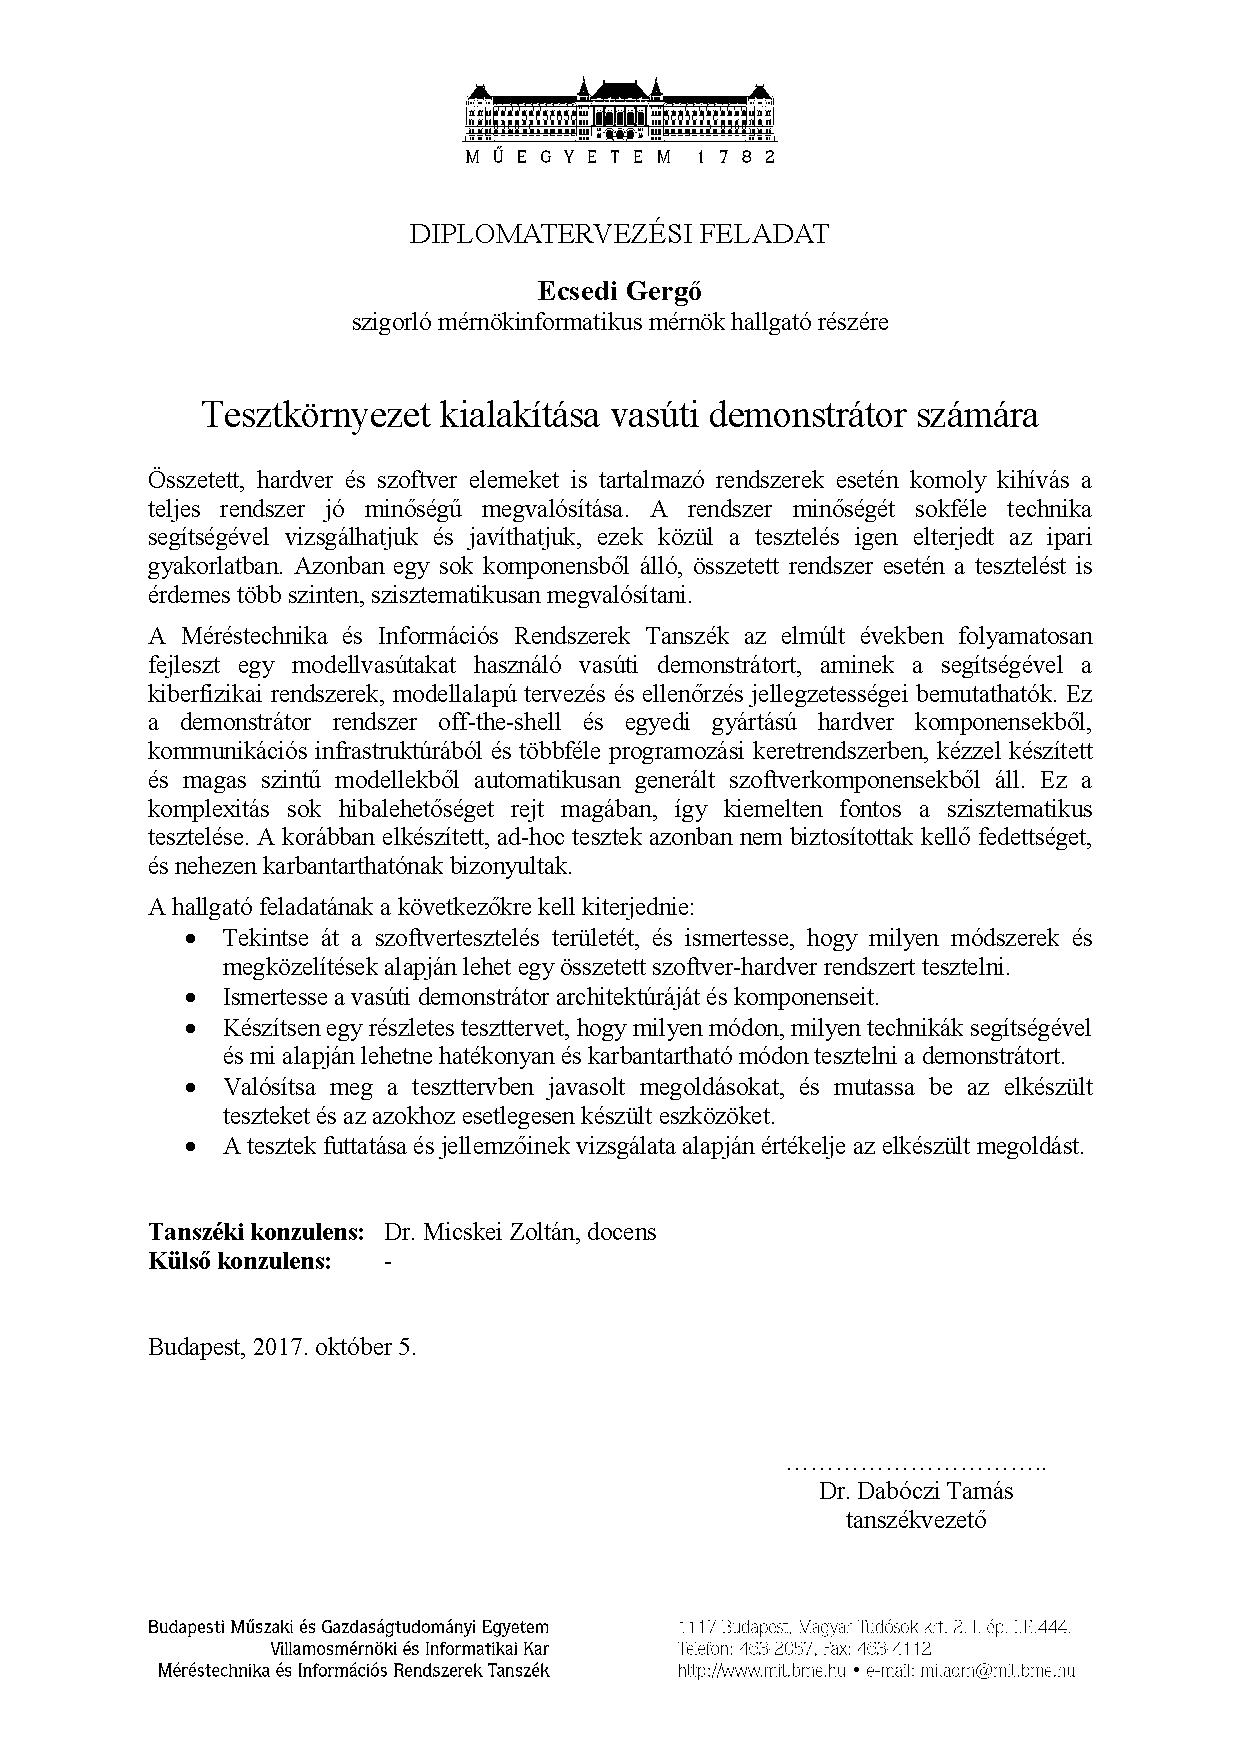
\includepdf[noautoscale]{content/Feladatkiiras.pdf}

%~~~~~~~~~~~~~~~~~~~~~~~~~~~~~~~~~~~~~~~~~~~~~~~~~~~~~~~~~~~~~~~~~~~~~~~~~~~~~~~~~~~~~~
\hypersetup{pageanchor=false}
%--------------------------------------------------------------------------------------
%	The title page
%--------------------------------------------------------------------------------------
\begin{titlepage}
\begin{center}

\includegraphics[width=60mm,keepaspectratio]{figures/bme_logo.pdf}\\
\vspace{0.3cm}
\textbf{\bme}\\
\textmd{\vik}\\
\textmd{\viktanszek}\\[5cm]

\vspace{0.4cm}
{\huge \bfseries \vikcim}\\[0.8cm]
\vspace{0.5cm}
\textsc{\Large \vikdoktipus}\\[4cm]

{
	\renewcommand{\arraystretch}{0.85}
	\begin{tabular}{cc}
	 \makebox[7cm]{\emph{\keszitette}} & \makebox[7cm]{\emph{\konzulens}} \\ \noalign{\smallskip}
	 \makebox[7cm]{\szerzo} & \makebox[7cm]{\vikkonzulensA} \\
	  & \makebox[7cm]{\vikkonzulensB} \\
	  & \makebox[7cm]{\vikkonzulensC} \\
	\end{tabular}
}

\vfill
{\large \today}
\end{center}
\end{titlepage}
\hypersetup{pageanchor=false}

		   % Szakdolgozat/Diplomaterv címlap
%%% TDK címlap
\begin{titlepage}
  \begin{center}  
  
\includegraphics[width=7cm]{./figures/bme_logo.pdf}
  \vspace{0.3cm}
  
  \bme \\
  \vik \\
  \viktanszek \\
  \vspace{5cm}
  
  \huge {\vikcim}
  \vspace{1.5cm}
  
  \large {\textbf{\vikdoktipus}}
  \vfill
    
  {\Large 
  	\keszitette: \\ \vspace{0.3cm}
  	\szerzo \\
	\tdkszerzoB \\
  	\vspace{1.5cm}
  	\konzulens: \\ \vspace{0.3cm}
  	\vikkonzulensA \\
  	\vikkonzulensB \\
  }
  
  \vspace{2cm}
  \large {\tdkev}
 \end{center}
\end{titlepage}
%% Címlap vége	% TDK címlap
%%% OTDK külső címlap
\begin{titlepage}
  	$\;$ 
	\vspace{5cm}
	
	\begin{center}
	\Huge
	\textbf{TDK-dolgozat}\let\thefootnote\relax\footnote{A dolgozat bemutatását a XXXXXXXXX  ``Lorem ipsum dolor sit amet'' című program támogatta.}
	\end{center}
	
	\vspace{13cm}
	
	\Large
	\hspace{8cm} \szerzo
	
	\hspace{8cm} \tdkszerzoB
	
	\hspace{8cm} \tdkev.
\end{titlepage}

\newpage
\thispagestyle{empty}


%% OTDK belső címlap
\begin{titlepage}
  \begin{center}  
  
\includegraphics[width=7cm]{./figures/bme_logo.pdf}
  \vspace{0.3cm}
  
  \bme \\
  \vik \\
  \viktanszek \\
  \vspace{3.5cm}
  
  \huge {\vikcim}
  \vspace{1.5cm}
  
  \large {\textbf{\vikdoktipus}}
  \vfill
    
  {\Large 
  	{\large \keszitette:} \\ \vspace{0.2cm}
  	\szerzo \\ \tdkevfolyamA. évfolyam \\
	\vspace{0.5cm}
	\tdkszerzoB \\ \tdkevfolyamB. évfolyam \\
  	\vspace{1.5cm}
  	{\large \konzulens:} \\ \vspace{0.2cm}
  	\vikkonzulensA,\\ \tdkkonzulensbeosztasA \\
  	\vspace{0.5cm}
  	\vikkonzulensB,\\ \tdkkonzulensbeosztasB \\
  }
  
  \vspace{2cm}
  \large {\tdkev.}
  
 \end{center}
\end{titlepage}   % OTDK címlap


% Table of Contents
%~~~~~~~~~~~~~~~~~~~~~~~~~~~~~~~~~~~~~~~~~~~~~~~~~~~~~~~~~~~~~~~~~~~~~~~~~~~~~~~~~~~~~~
\tableofcontents\vfill


% Declaration and Abstract
%~~~~~~~~~~~~~~~~~~~~~~~~~~~~~~~~~~~~~~~~~~~~~~~~~~~~~~~~~~~~~~~~~~~~~~~~~~~~~~~~~~~~~~
\selectlanguage{magyar}
\pagenumbering{gobble}
%--------------------------------------------------------------------------------------
% Nyilatkozat
%--------------------------------------------------------------------------------------
\begin{center}
\large
\textbf{HALLGATÓI NYILATKOZAT}\\
\end{center}

Alulírott \emph{\vikszerzoVezeteknev{} \vikszerzoKeresztnev}, szigorló hallgató kijelentem, hogy ezt a \vikmunkatipusat{} meg nem engedett segítség nélkül, saját magam készítettem, csak a megadott forrásokat (szakirodalom, eszközök stb.) használtam fel. Minden olyan részt, melyet szó szerint, vagy azonos értelemben, de átfogalmazva más forrásból átvettem, egyértelműen, a forrás megadásával megjelöltem.

Hozzájárulok, hogy a jelen munkám alapadatait (szerző(k), cím, angol és magyar nyelvű tartalmi kivonat, készítés éve, konzulens(ek) neve) a BME VIK nyilvánosan hozzáférhető elektronikus formában, a munka teljes szövegét pedig az egyetem belső hálózatán keresztül (vagy autentikált felhasználók számára) közzétegye. Kijelentem, hogy a benyújtott munka és annak elektronikus verziója megegyezik. Dékáni engedéllyel titkosított diplomatervek esetén a dolgozat szövege csak 3 év eltelte után válik hozzáférhetővé.

\begin{flushleft}
\vspace*{1cm}
Budapest, \today
\end{flushleft}

\begin{flushright}
 \vspace*{1cm}
 \makebox[7cm]{\rule{6cm}{.4pt}}\\
 \makebox[7cm]{\emph{\vikszerzoVezeteknev{} \vikszerzoKeresztnev}}\\
 \makebox[7cm]{hallgató}
\end{flushright}
\thispagestyle{empty}

\vfill
\clearpage
\thispagestyle{empty} % an empty page

\selectthesislanguage
 
\pagenumbering{roman}
\setcounter{page}{1}

\selecthungarian

%----------------------------------------------------------------------------
% Abstract in Hungarian
%----------------------------------------------------------------------------
\chapter*{Kivonat}\addcontentsline{toc}{chapter}{Kivonat}




\vfill
\selectenglish


%----------------------------------------------------------------------------
% Abstract in English
%----------------------------------------------------------------------------
\chapter*{Abstract}\addcontentsline{toc}{chapter}{Abstract}




\vfill
\selectthesislanguage

\newcounter{romanPage}
\setcounter{romanPage}{\value{page}}
\stepcounter{romanPage}    


% The main part of the thesis
%~~~~~~~~~~~~~~~~~~~~~~~~~~~~~~~~~~~~~~~~~~~~~~~~~~~~~~~~~~~~~~~~~~~~~~~~~~~~~~~~~~~~~~
\pagenumbering{arabic}

%TODO import your own content
%----------------------------------------------------------------------------
\chapter{\bevezetes}
%----------------------------------------------------------------------------



%----------------------------------------------------------------------------
\chapter{Railway demonstrator system architecture}
%----------------------------------------------------------------------------
In this chapter I want to describe the railway demonstrator system, which is shown in figure \ref{fig:overview}. This system's purpose is to simulate a real-life safety critical railway system, with basic functionalities and train collision detection. The demonstrator is based on a railway model stub which is extended with custom and off-the-shelf hardware, software components. 
\begin{figure}[h]
	\centering
	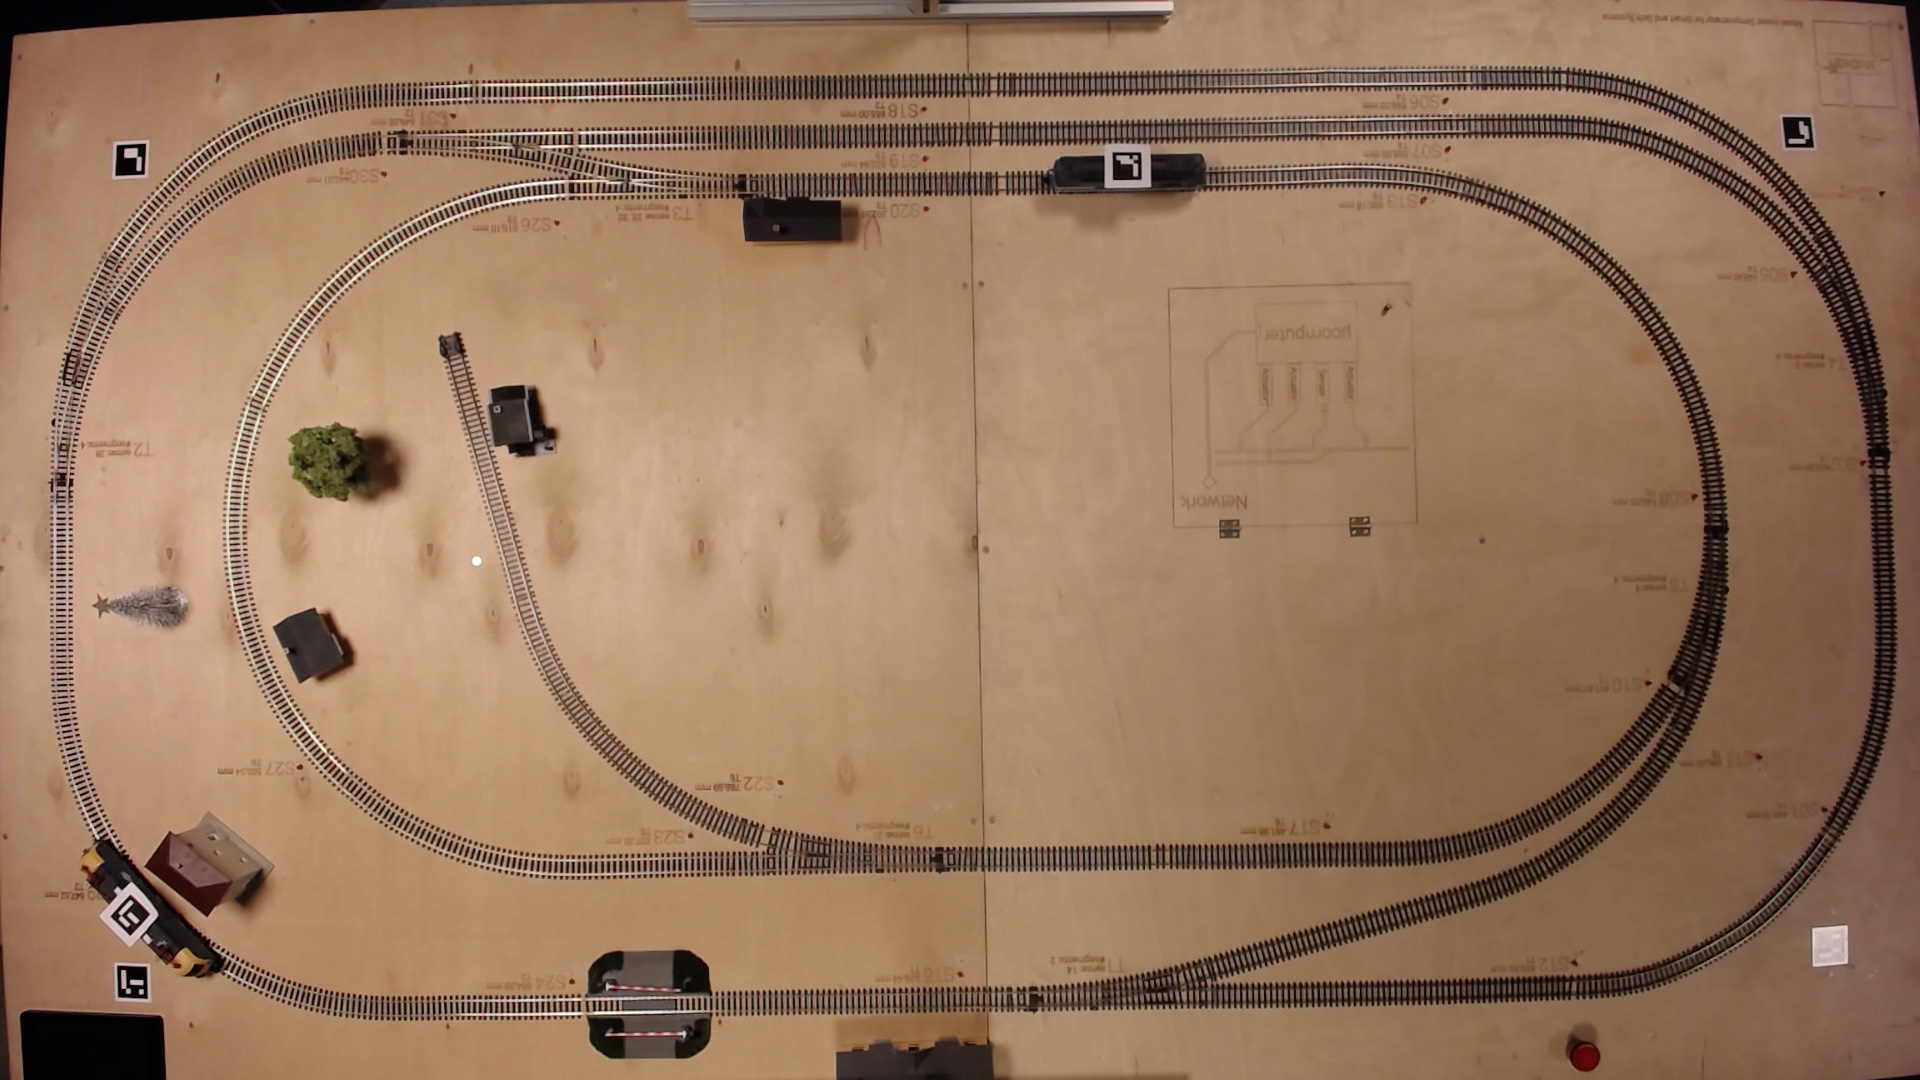
\includegraphics[width=150mm]{figures/modes3/overview.jpg}
	\caption{Railway system overview}
	\label{fig:overview}
\end{figure}

\section{Railway system basic components}
First of all I want to introduce the physical components and the basic process of the railway systems stub. There are 31 sections, with one blind track and 7 turnouts. The \ref{fig:layout} figure shows the layout of railway elements with corresponding segment ids. Over all a segment means either section or turnout.
\todo[inline]{Create more visible figure about layout}

\begin{figure}[h]
	\centering
	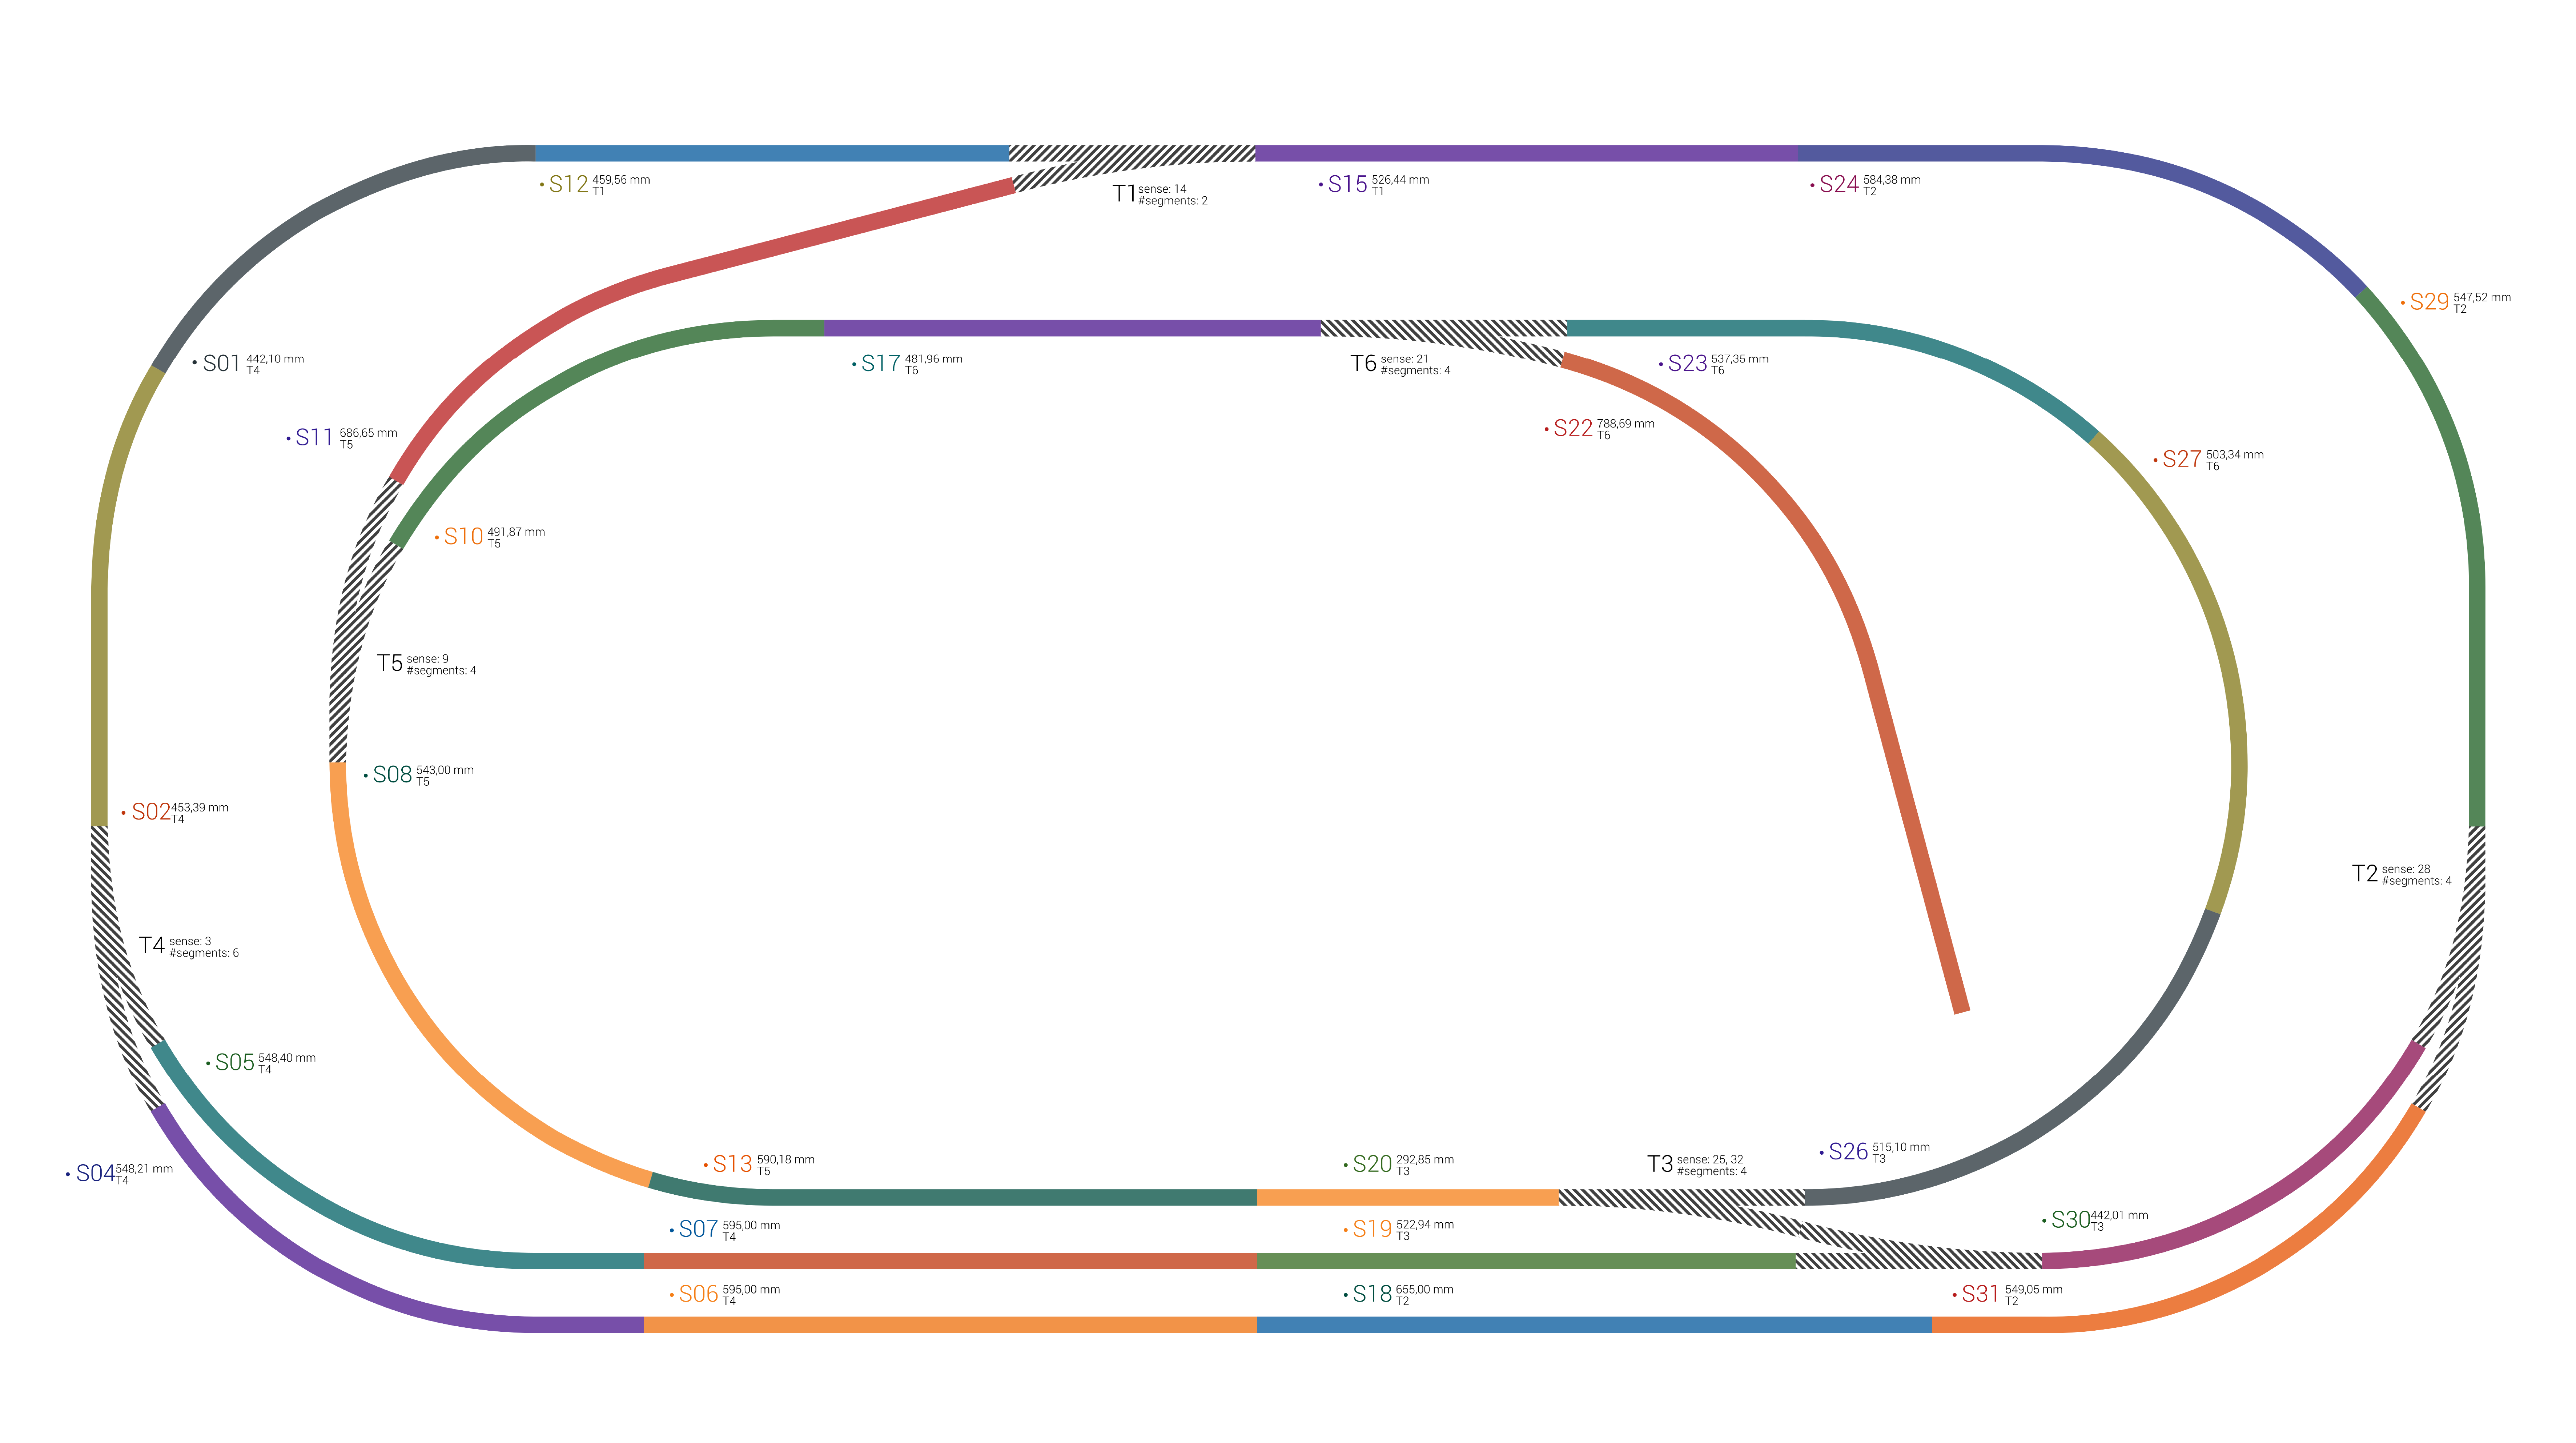
\includegraphics[width=150mm, keepaspectratio]{figures/modes3/layout2.png}
	\caption{Railway layout}
	\label{fig:layout}
\end{figure}

\paragraph{Section} 
First principal  element is a 15-20 cm long railroad. Each section is connected to 2 other sections, and wired to a command station which gives them sufficient power source for moving the trains. In the figure \ref{fig:layout} these sections are identified by \textit{SXX} strings, where \textit{XX} is two unique digits for this layout. Furthermore these numerals determines which bit shows this section's occupancy in the occupancy vector later (see section \ref{section:OccupancyDetection} for more information). On the \ref{fig:layout} figure for each section lengths and responsible BeagleBone Black ids are shown.

\paragraph{Turnout}
Second principal element is the turnout, which can differentiate 2 paths on the track as it can be seen on figure \ref{fig:turnoutDir}. The train which is going through a turnout can reach different sections depending on the state of the exact turnout. On the layout figure (\ref{fig:layout}) each of these elements are visible as gray dashed sections with the IDs. Each turnout ID starts with T and ends with a numeric (1..6). These IDs determines, which bit identifies the turnout's occupancy in the occupancy vector) and \textit{\#segments} as number of supervised sections by the BeagleBone Black (see section \ref{section:OccupancyDetection} for more information about occupancy vector).
\begin{figure}[!h]
	\centering
	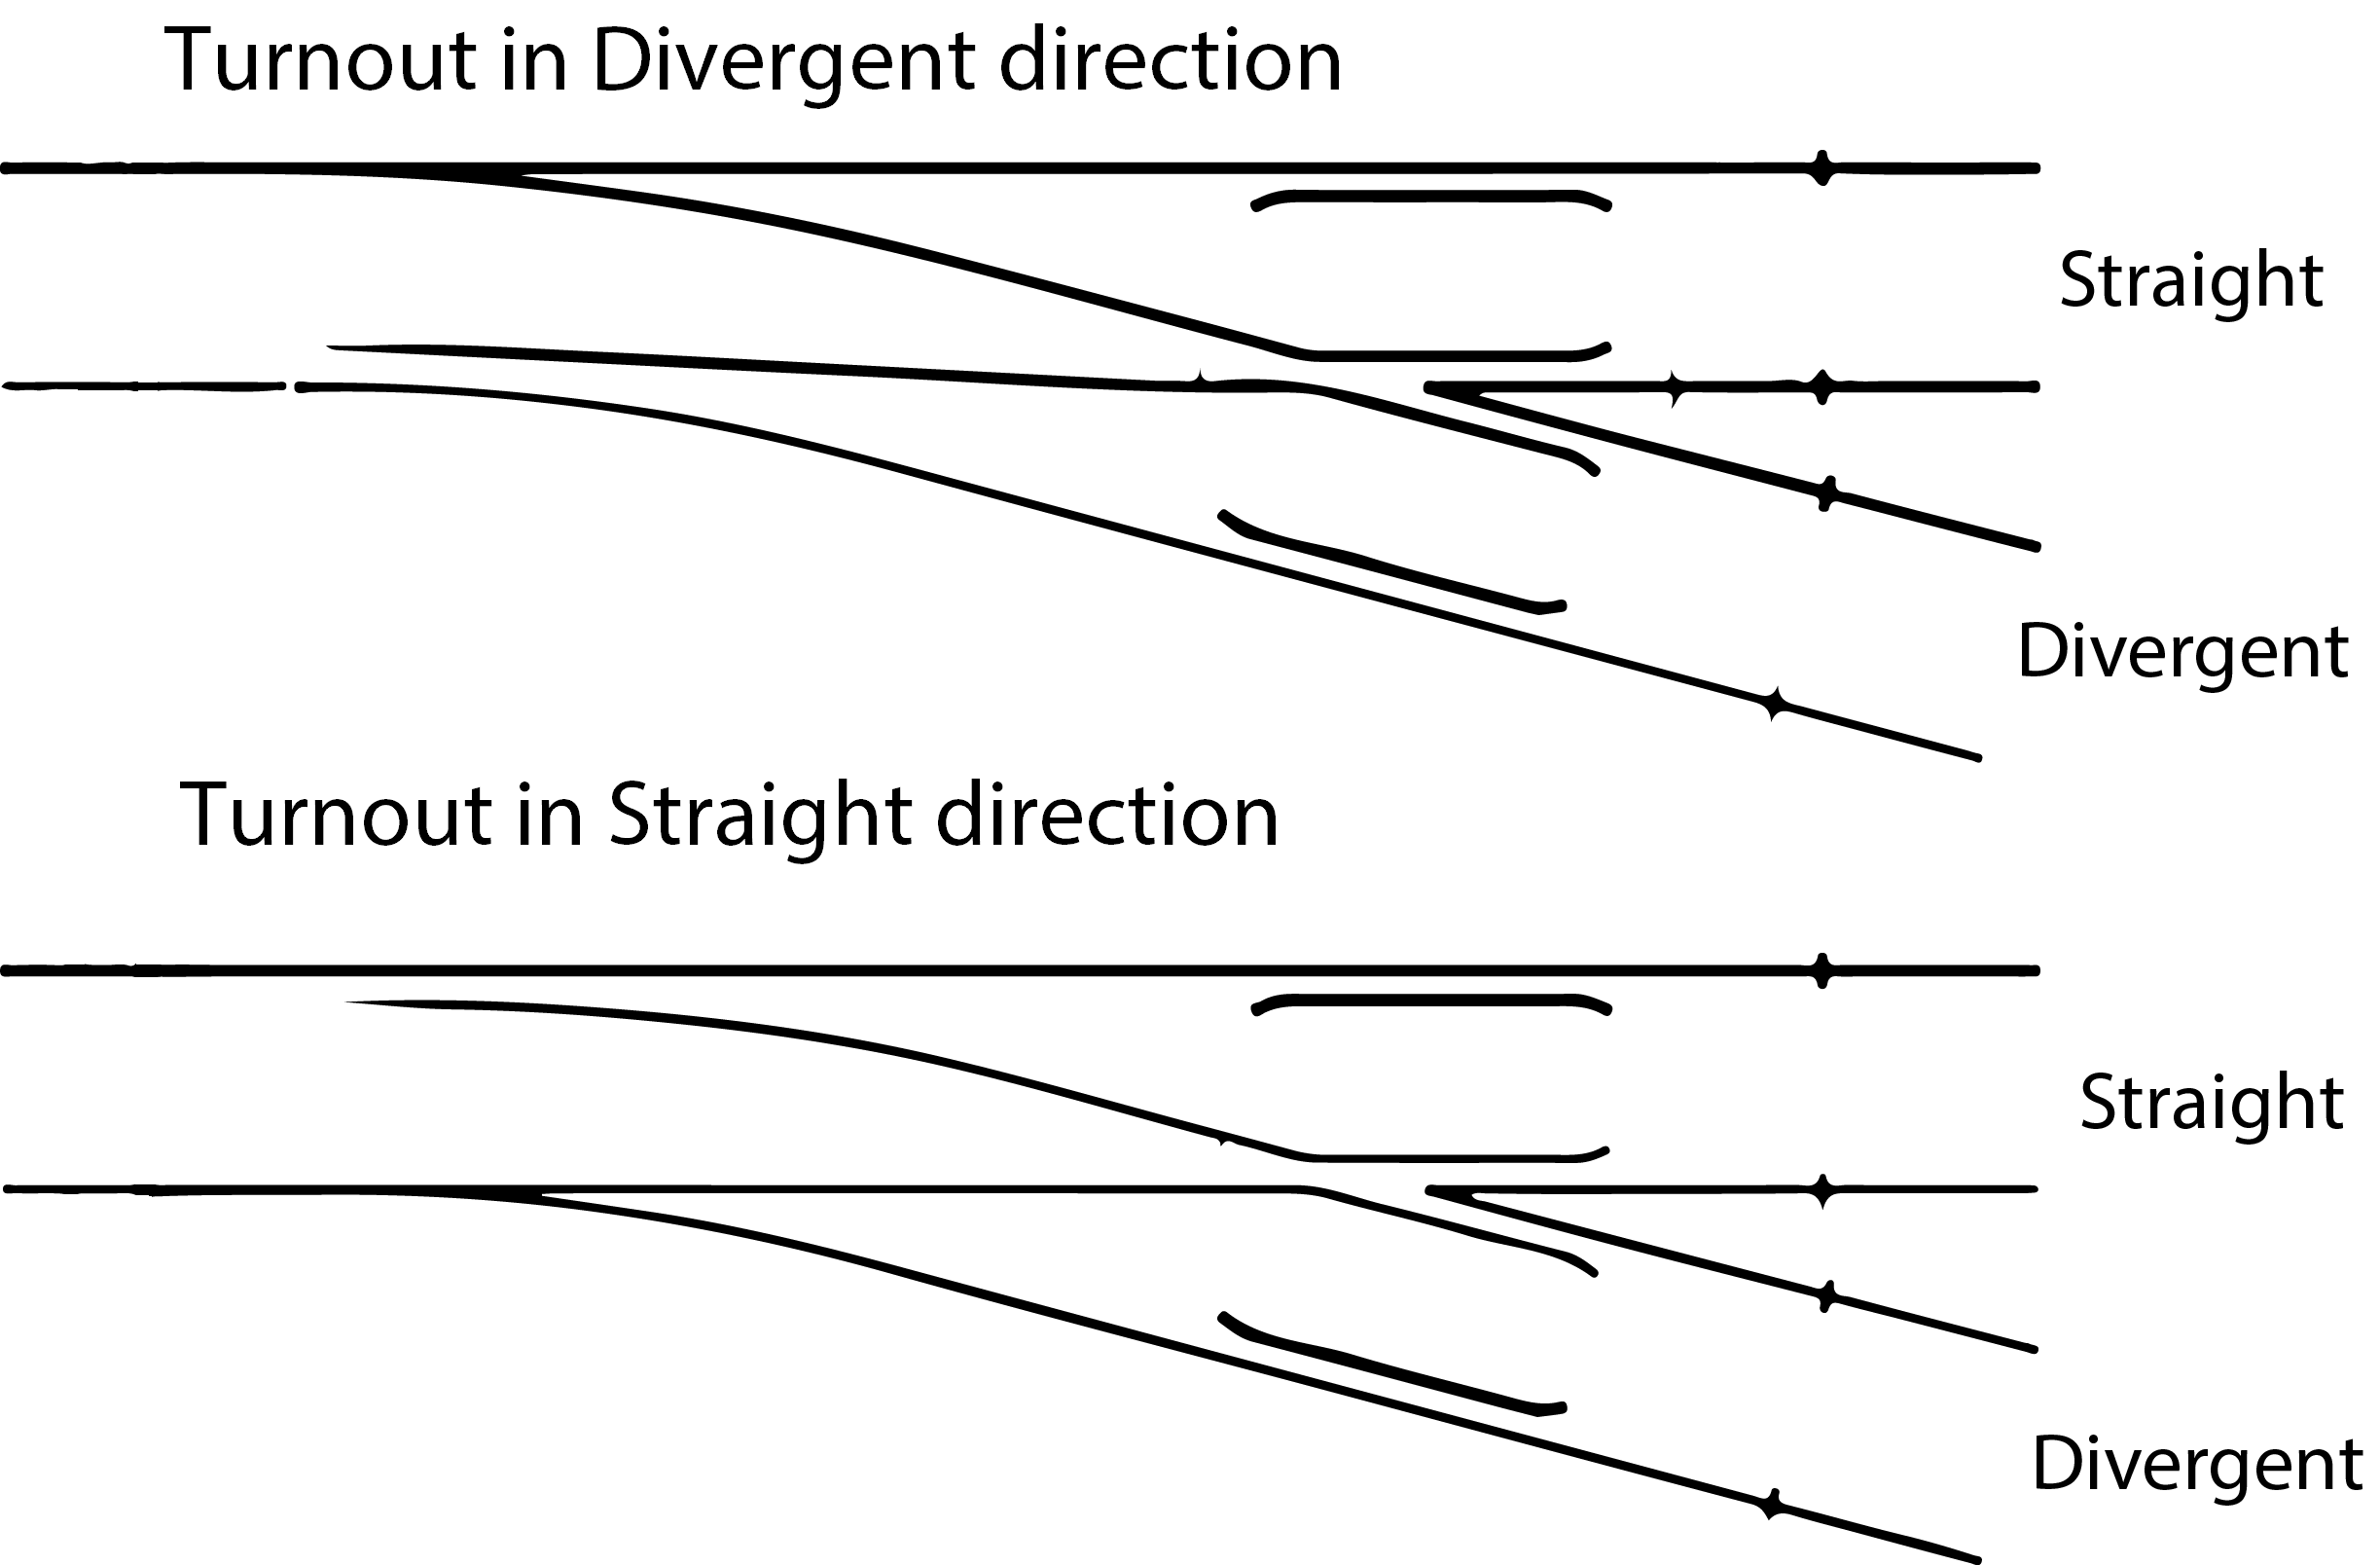
\includegraphics[width=150mm]{figures/modes3/turnout.png}
	\caption{Turnout directions}
	\label{fig:turnoutDir}
\end{figure}

\paragraph{Train} \label{par:trainScenarios}
There are 2 model trains in the system, which can move on the sections and turnouts. The first safety critical paradigm is to avoid a train collision on the track, for which the basic scenarios are the following. 

\todo[inline]{Move the collision scenarios to a new chapter}

First approach is that 2 trains are passing through the same turnout, from the same direction on different paths. It means that they are approaching the same section of the turnout, so they will collide like on the \ref{fig:LayoutT1-scenario1} figure.
\begin{figure}[!h]
	\centering
	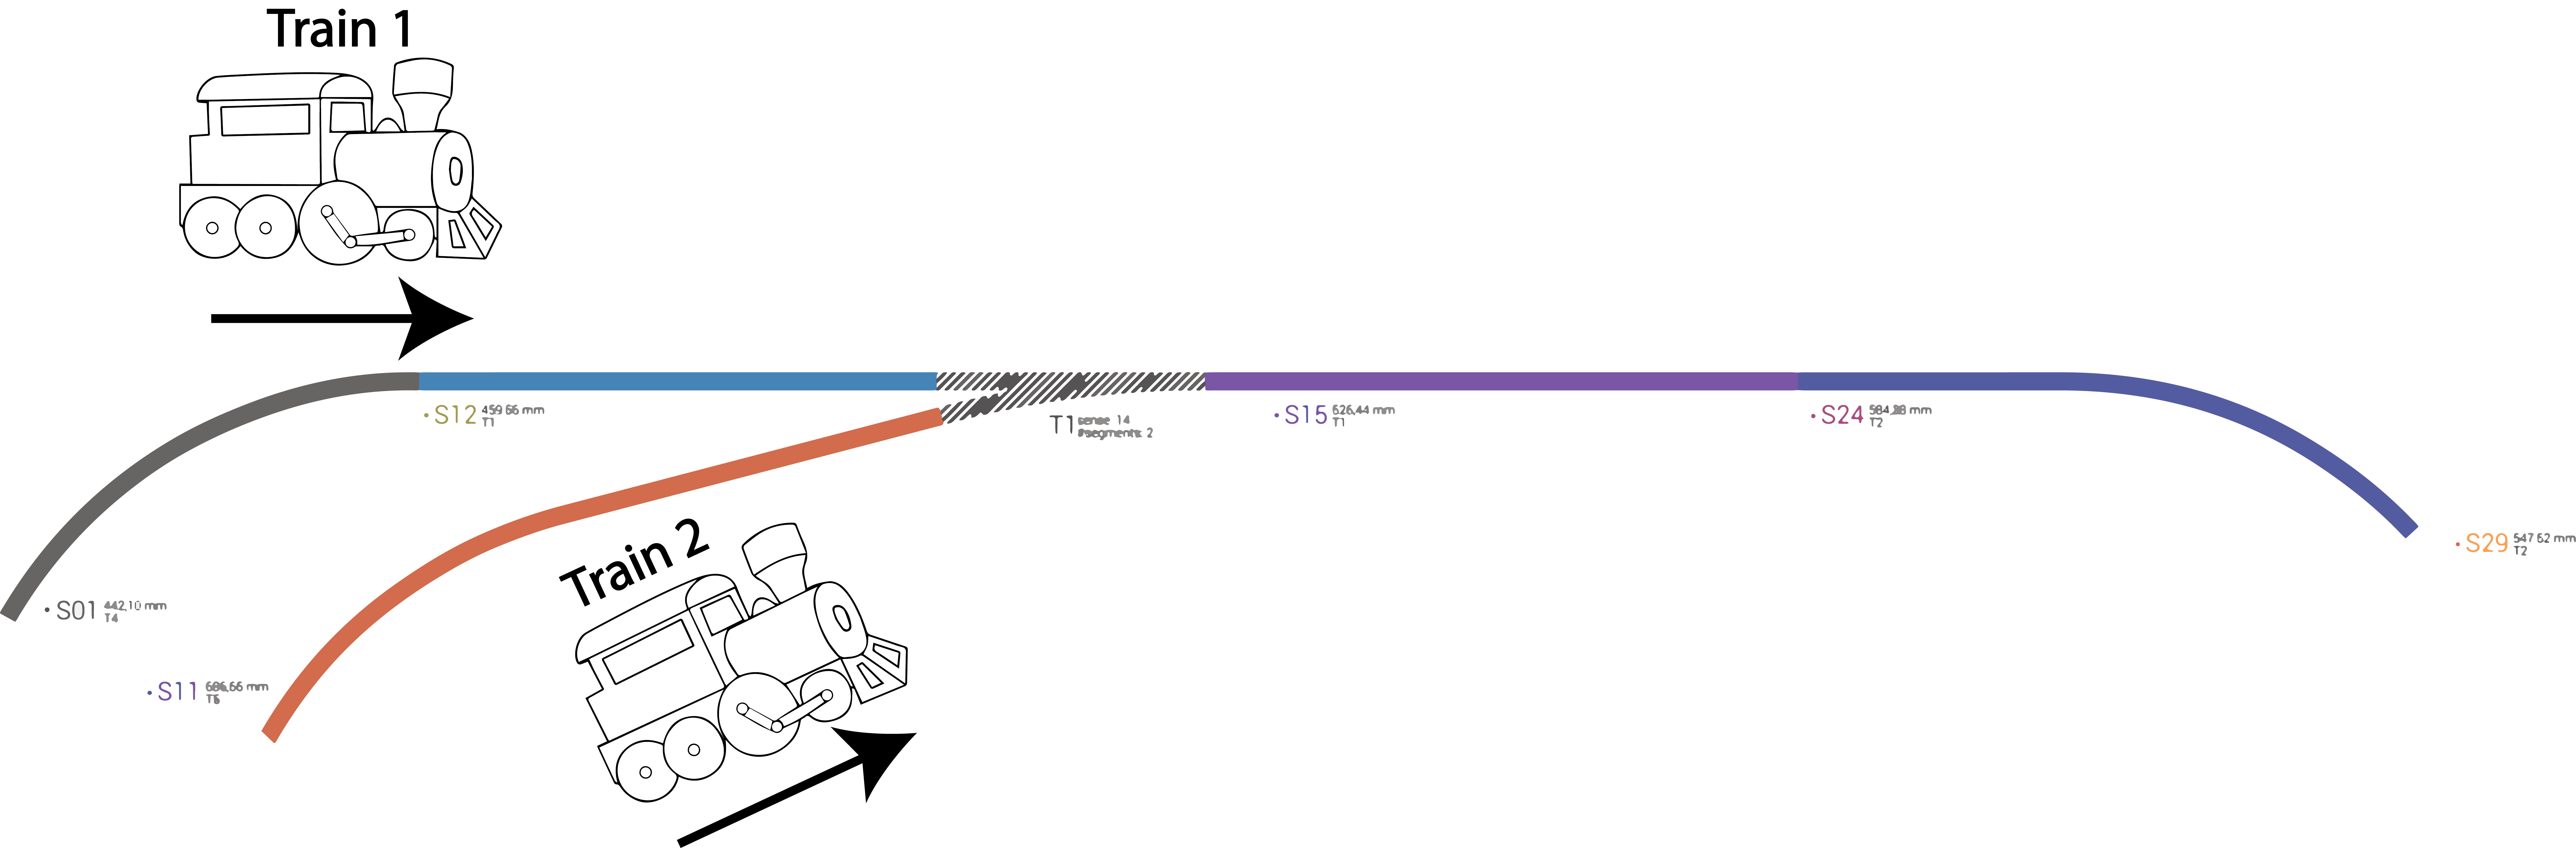
\includegraphics[width=150mm, keepaspectratio]{figures/modes3/layoutT1-scenario1.png}
	\caption{Turnout 1 collision scenario 1}
	\label{fig:LayoutT1-scenario1}
\end{figure}

Next possible scenario is shown in \ref{fig:LayoutT1-scenario2} figure, when \textit{Train 1} is going to the section where \textit{Train 2} is staying. Notice that no matter in which direction the \textit{Train 2} is moving or staying, it is a dangerous situation.
\begin{figure}[!h]
	\centering
	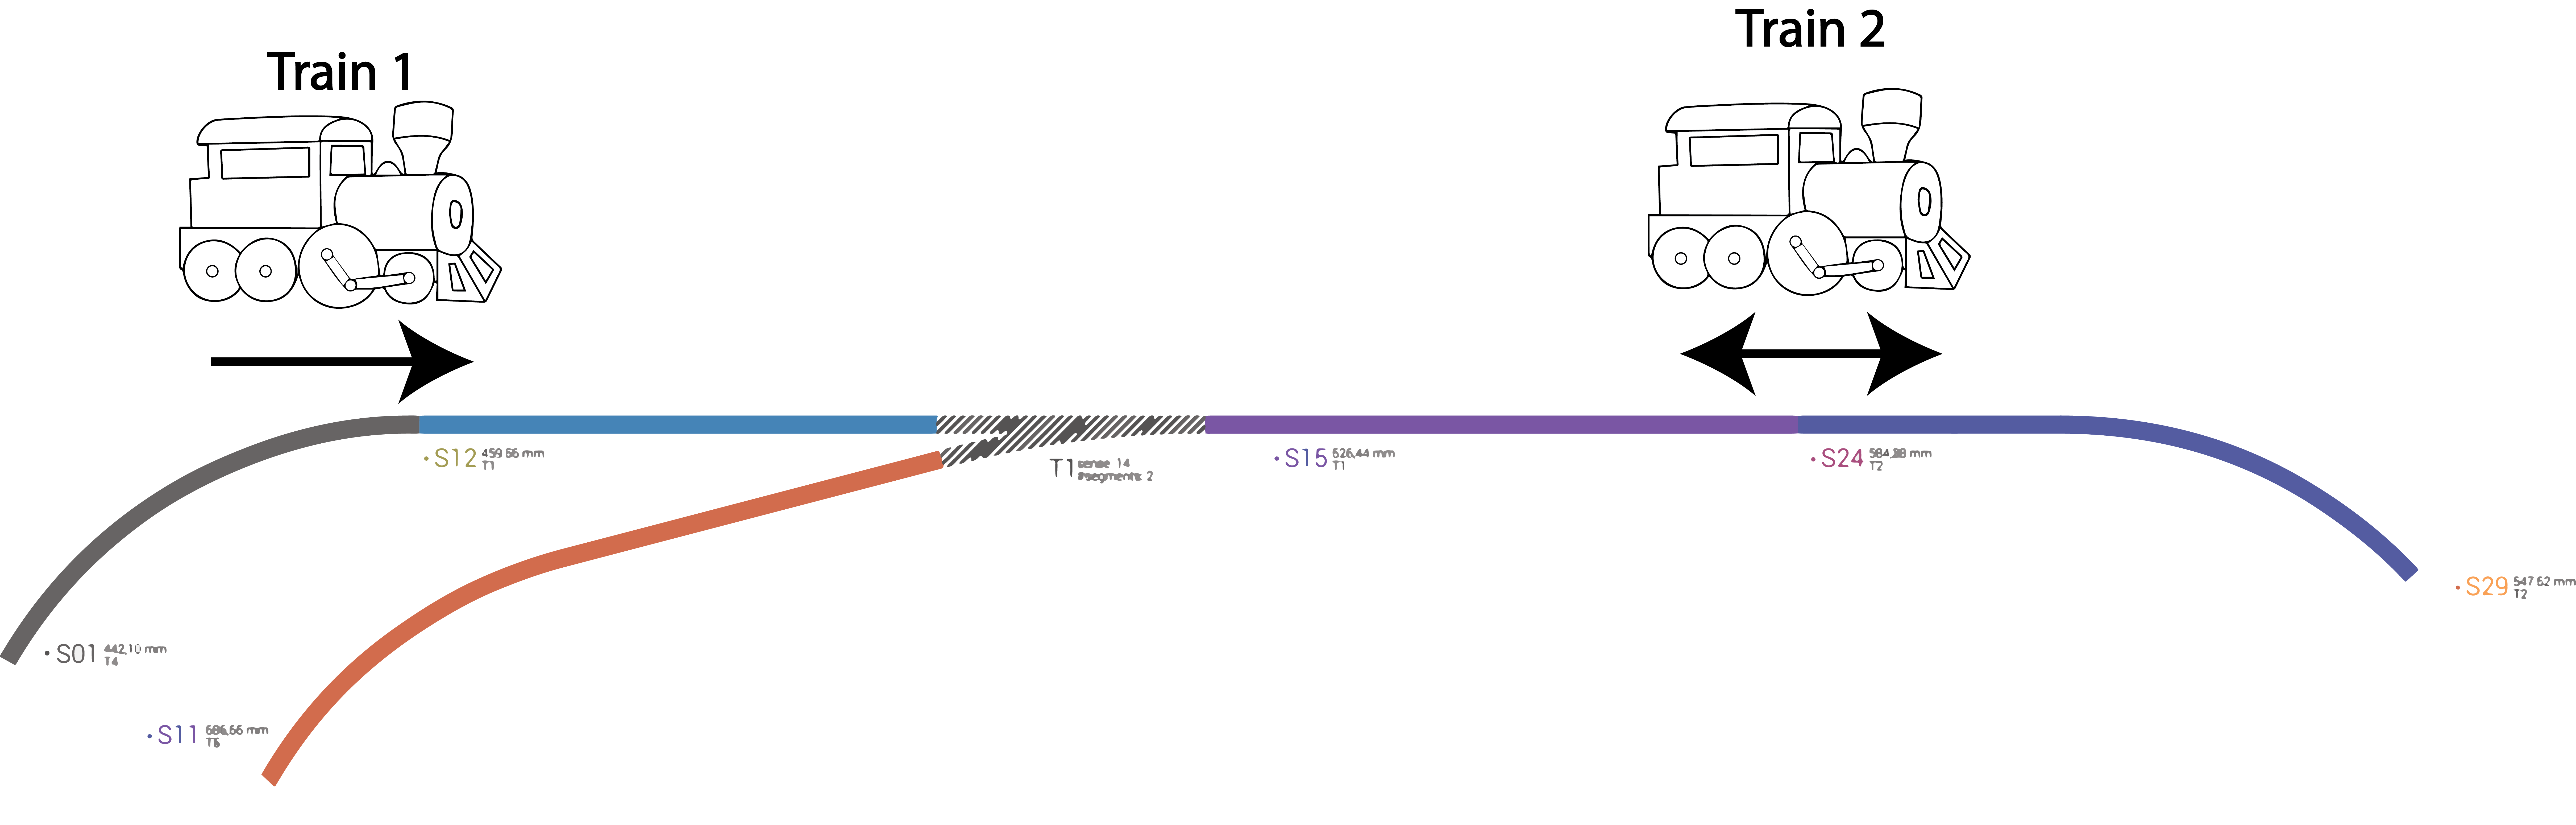
\includegraphics[width=150mm, keepaspectratio]{figures/modes3/layoutT1-scenario2.png}
	\caption{Turnout 1 collision scenario 2}
	\label{fig:LayoutT1-scenario2}
\end{figure}

\paragraph{Command Station}
Supply power source for the sections which provides tension for the trains on the track.

\paragraph{Controller}
In connection with the \textit{Command Station} an XPressNet protocol \footnote{More details about XPressNet Protocol \url{http://www.lenzusa.com/1newsite1/Manuals/xpressnet.pdf}} based controller is attached to the system. This component's purpose is setting the direction and speed for each train on the track.

\section{Hardware extensions}
The basic hardware environment is not sufficient for controlling and analyzing purposes, therefore additional hardware elements have been designed to satisfy these requirements. In this section these platforms will be described in details. (The \ref{appendix:HWPictures} appendix contains pictures about the elements.)
\todo[inline]{Check if these infos are necessary and where to put them}
For modeling purposes I have used MagicDraw with Sysml plugin \cite{SysML}.

\subsection{Data processing units}
\begin{figure}[h]
	\centering
	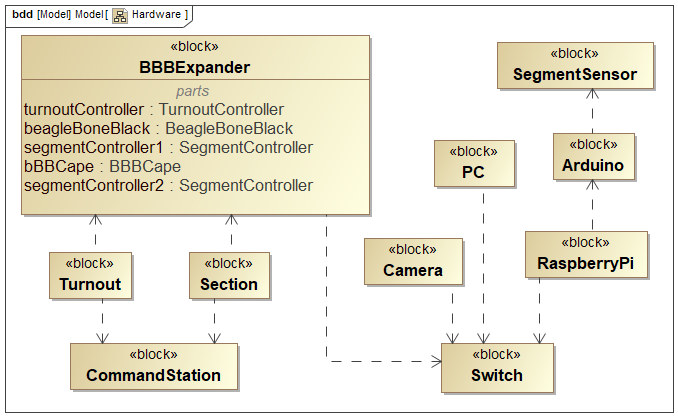
\includegraphics[width=150mm]{figures/modes3/Hardware.png}
	\caption{Hardware block definition diagram}
	\label{fig:Modes3HWBDD}
\end{figure}

\paragraph{BeagleBone Black (BBB)}
An industrial microcontroller platform which provides 4GB 8-bit eMMC on-board flash storage and 2x PRU 32-bit microcontrollers, which could satisfy the function for parallel monitoring. There are 6 BBB on the track connected to the railway, used for controlling and enabling/disabling each section.

\paragraph{Rapsberry Pi 3}
A Rapsberry Pi microcontroller is dedicated to handle most of the software components related to the Railway demonstrator system. It has twice as large computing capacity in RAM and also in CPU as BBB.

\paragraph{Arduino}
Dedicated hardware element for reading from the 6 DigiSens-8-S88 output data through S88 protocol (see \ref{par:SegmentSensor} section for details about this component). This communication layer requires proper timing conditions which the Arduino platform can satisfy.

\subsection{Custom hardware extensions}
\paragraph{BeagleBone Black cape and expanders}\label{par:BBBcape}
The BeagleBone Black components expect 5VDC power source instead of 12VDC which our power station supplies. Because of that reason a so called cape have been created for each controller. Additionally the need for easy-to-use ports to attach additional circuits to the main board also have come up. The expanders could be used to extend the functionality of one BeagleBone unit, which is on the figure \ref{fig:capeSysml}. 
\todo[inline]{More suitable figure here for BBB expendable interfaces}
\begin{figure}[!h]
	\centering
	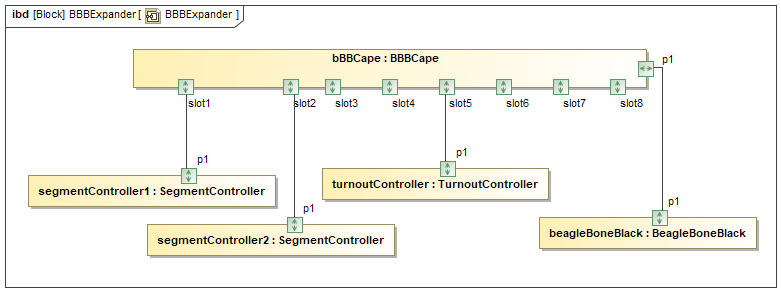
\includegraphics[width=150mm]{figures/modes3/BBBExpander.png}
	\caption{Layout and current attachment of cape and expander}
	\label{fig:capeSysml}
\end{figure}

Each cape have 8 general purpose expander slot, for which the pin layout is expressed in the following \ref{table:expander_pin_layout} table.

\begin{table}[!h]
	\caption{Pin layout}
	\label{table:expander_pin_layout}
	\begin{center}
		\renewcommand{\arraystretch}{1.5}
		\begin{tabu} to 0.5\textwidth { | X[c] | X[c] | X[c] | X[c] |}
			\hline
			pin3 & pin2 & pin1 & pin0 \\
			\hline
			3V3  & 5V  & Gnd  & 12V\\
			\hline
		\end{tabu}
	\end{center}
\end{table} 

\todo[inline]{Give proper details about G0-G15 pins, the table is not showing all of them like \url{https://github.com/FTSRG/BME-MODES3/wiki/HW-Expander-design}}  

The upper row of each connector is dedicated for GPIO connections. Two of the GPIO pins connected to the application processor and the remaining two GPIO pins are connected to the PRU unit.

With this setup, the PRU and the application processor can cooperate on hardware level.

\paragraph{Segment sensor}\label{par:SegmentSensor}
The DigiSens-8-S88 component is an off-the-shelf product, which can detect the occupancy for 8 segments. \footnote{More information about the product can be found here:\url{http://www.digitools.hu/termekek/erzekelok/digisens-8-s88}}.

\paragraph{Segment actuator}
Segment Actuator expanders are designed to stop a train on the corresponding segment. The concept behind this expander based on the Lenz Asymmetrical DCC and ABC functionality of train-decoders. \footnote{The following descriptions are based on \url{https://tonystrains.com/lenz-asymmetrical-dcc-and-abc/} article.}

%
%ABC (Automatic Brake Control) works in conjunction with Asymmetrical DCC. Asymmetrical DCC is a way to trigger ABC in the decoder. This gives the ability to stop trains at a section of the track with Asymmetrical DCC.

%\begin{figure}[!h]
%	\centering
%	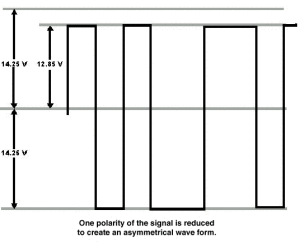
\includegraphics[width=100mm]{figures/modes3/DCC.png}
%	\caption{Asymmetric DCC voltages}
%	\label{fig:dcc}
%\end{figure}

%The Asymmetrical DCC signal is generated by offsetting one phase of the DCC signal. This signal then triggers the Automatic Brake Control in the decoder. This causes the engine to stop at the distance set up in the Constant Stopping Distance feature. We implemented this using five diodes. %connected in the form as shown in the figure below.
%\begin{figure}[h]
%	\centering
%	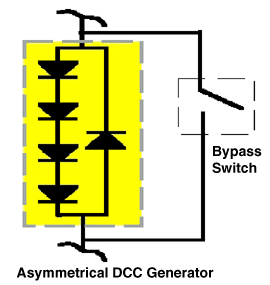
\includegraphics[width=50mm]{figures/modes3/abc.png}
%	\caption{Asymmetric DCC voltages}
%	\label{fig:abc}
%\end{figure}

The Segment Actuators uses this setup and also gives an interface (with GPIOs) to enable or disable this feature. Every Segment Actuator expander has two slots (A or B) and can enable or disable two segments. Each segment can be enabled setting two GPIOs to HIGH level, one connected to the PRU and one connected to the application processor.

\paragraph{Turnout actuator}
Turnout Actuator expanders can switch turnouts on the table between their states. Previously, we have managed to solve this with COTS (Commercial off-the-shelf) units, but in that case we were not able to query the position of the switch programmatically. This expander gives the ability for both switching the turnout and sensing its state.

The concept behind this unit is based on the fact, that turnout mechanism is working as a wire between the common (COM) pole and an other pole (STR or DIV) when switched in one position, therefore we can sense its state.

The electronic characteristics of the BeagleBone unit could not satisfy the switching process electrically, thus we had to use a micro-controller (an Atmega328 MCU). Also, the state-sensing process is based on Analog to Digital Converters, which are also integrated into the MCU.

\textbf{Usage}
The MCU has 2 inputs and 2 outputs connected to the expander connector as shown in the table below.
\begin{center}
	\renewcommand{\arraystretch}{1.5}
	\begin{tabu} to 1.0\textwidth {X[c] X[c] X[c] X[c]}
		\toprule
		Pin 0                                  & Pin 1                                   & Pin 2                           & Pin 3                             \\ \midrule
		Turnout switching to Straight position & Turnout switching to Divergent position & Turnout state sensing (Straing) & Turnout state sensing (Divergent) \\
		INPUT for the MCU                      & INPUT for hte MCU                       & OUTPUT for the MCU              & OUTPUT for the MCU                \\ \bottomrule
	\end{tabu}
\end{center}


\section{Software components}
\todo[inline]{update the figure with traindetector and delete physical controllers}
\begin{figure}[h]
	\centering
	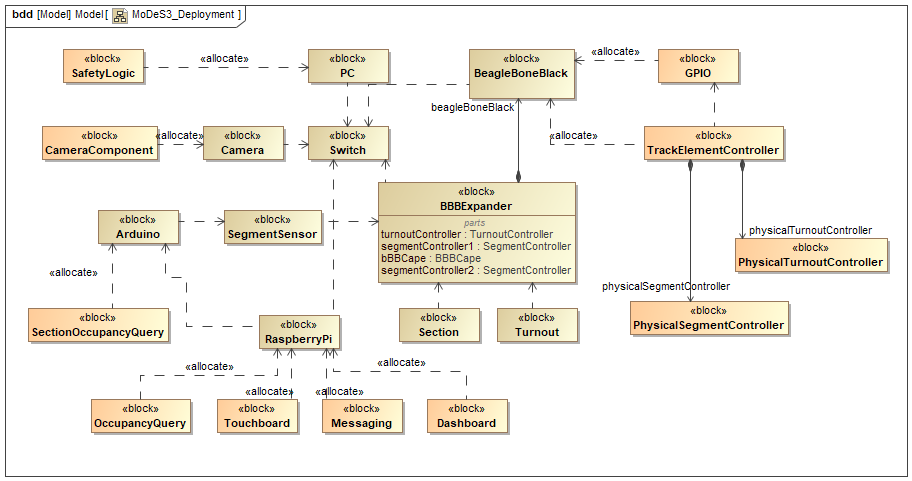
\includegraphics[width=150mm]{figures/modes3/MoDeS3_Deployment1.png}
	\caption{Software components deployment to hardware elements}
	\label{fig:Modes3Deployment}
\end{figure}

\subsection{Occupancy detection elements} \label{section:OccupancyDetection}
\paragraph{Section Occupancy Query}
Responsible for debouncing the 32bit long occupancy vector with proper timing conditions regarding S88 protocol and forward this 32bit to \textit{Occupancy Query} through usb connection. Computed data contains the occupancy information for each track element (section or turnout) per one bit.
\paragraph{Occupancy Query}
In connection with the \textit{Section Occupancy Query} process the occupancy state for the whole track. Only if the state has changed, it sends occupancy change message to the MQTT topic with the track element id and new occupancy state.

\subsection{Track segment control elements}
\paragraph{GPIO}
Handles the GPIO pin changes and commands for each extension point of the BBB cape (see \ref{par:BBBcape} section for details about BBB cape and expanders).
\paragraph{Track Element Controller}
On each BeagleBone Black microcontroller there is a controller, which executes the turnout and segment operations for the supervised sections. To satisfy this functionality this controller forwards commands to the corresponding Physical Segment or Turnout Controllers, which communicates with GPIO managers. Consequently with this platform specific software, we are able to enable or disable sections and set turnout directions.
\paragraph{Train Detector}
Train detector and locomotive length measurer using infrared sensors.

\subsection{Track control and supervisor elements}
\paragraph{XPressNet}
Protocol for sending messages to the \textit{Command Station} component, therefore we can extend the communication form for controlling the track. In the current layout there is a controller and web-based opportunity for controlling.
\paragraph{Dashboard}
Model railway track dashboard implementation, where we can manipulate the track elements. In Addition this component is instantiated only once, and up for the whole time while the track is in use. Consequently we can reach one common dashboard from the web and it contains the actual occupancy and track element status.
\paragraph{Touch board}
Dashboard for the model railway track, with focus on touchable elements, that can be controlled.
\paragraph{Safety Logic}
In the MODES$^3$ safety critical project we want to avoid the collision of model trains, therefore the safety logic software component detects these critical scenarios by Viatra Query \cite{Viatra} patterns and act the necessary action (for example disable a section).

\subsection{Messaging elements}
Each software component share information about the railroad system through the messaging software element, which is based on protobuf messages and provides high-level designed API with MQTT for this purpose. 
\begin{figure}[!h]
	\centering
	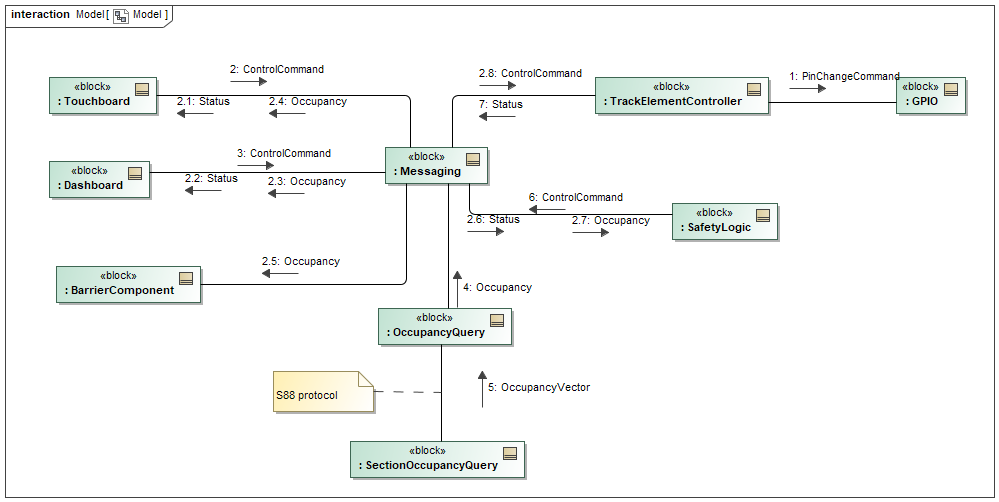
\includegraphics[width=150mm, keepaspectratio]{figures/modes3/CommunicationModel.png}
	\caption{Communication between software components}
	\label{fig:communicationModel}
\end{figure}

Separated topics are created for different information flow, and any component can subscribe for these topics. Basically on all topic, the information reporting is change based, so all components sending an information message to the dedicated topic when their state have changed (like occupancy changed or turnout changed). In opposite to that, there is a \textit{SendAllStatusCommand} which is a request for every component to send their actual status.

I will now list the specific MQTT topics and the connected software components to that, so basically what kind of information is flowing on them. (See software component connections on figure \ref{fig:communicationModel})

\paragraph{Segment Occupancy topic}
On this topic the \textit{Occupancy Query} component sending information whether an occupancy state is changed on any segment. (Notice that a segment can also be a section or a turnout too.) Most of the components are subscribed for this information topic so the \textit{Touch board}, \textit{DashBoard}, \textit{Barrier} (only for the supervised segments), \textit{Track Element Controller} and \textit{Safety Logic}.

\paragraph{Segment and Turnout Command topic}\label{par:MQTTTopicCommand}
Basically the \textit{Track Element Controller} process and accomplish these commands, and \textit{Touch board}, \textit{Dashboard} and \textit{Safety Logic} components can give these instructions.

\paragraph{Segment and Turnout Status topic}\label{par:MQTTTopicStatus}
For every command the \textit{Track Element Controller} will give a status acknowledgment message with the new state of the turnout or section. In this way the \textit{Touch board}, \textit{Dashboard} and \textit{Safety Logic} elements will be informed about the latest and current state.

\paragraph{CV topic}
The camera notification is communicated on that topic, which is received by the \textit{Safety Logic}.

\paragraph{ALL topic}
For this specific topic all the components in the system are subscribed, and information about train controlling and \textit{Command Station} related messages are shared.

\subsection{Complementary elements}
\paragraph{Barrier} 
Sends open/close commands to the barrier over the network, depending on the occupancy of supervised segments.
\paragraph{Leapmotion}
Software component for converting gestures into special movements for changing the speed of a specific train.

\section{Safety-critical functionalities}
\todo[inline]{Maybe figure of the Sw-Hw sysml for each paragraph}
\paragraph{Occupancy detection}\label{par:FunctionOccupancyDetection}
In order to know where are the trains on the track, we first must know which track elements (section or turnout) is occupied. This attribute can be determined whether the specific section has power consumption, which is used by train on it. The actual detection is made by the \textit{DigiSens-8-S88} sensing element. The demonstration railway system have four sensing element, and they are connected to an \textit{Arduino} S88 port. This microcontroller computes basic calculations by \textit{Section Occupancy Query} C++ software component and forwards the 32-bit occupancy vector information (actual state of every track element) to the \textit{Occupancy Query} via USB. The\textit{ Occupancy Query} Java component on the \textit{Rapsberry Pi} stores the previous occupancy state, and sends information to the \textit{Segment Occupancy} topic.

\paragraph{Track element controlling}\label{par:FunctionTEC}
For safety critical purposes in any collision scenario it is a good manner to disable all track elements, which is affected in the critical scenario. To make this switch possible, we have to cut the electric circle between the segment and \textit{Command Station}. The \textit{Section Controller} hardware element have been developed for changing a section,  the \textit{Turnout Controller} is responsible for changing a turnout. These hardware elements are attached to a \textit{BBB cape}, which is designed for supplying extension ports for BBB. In software point of view, through GPIO pins (specific file writing), we can give impulses from the BBB to the section or turnout. Therefore a \textit{GPIO manager} component is responsible for that in connection with the \textit{Track Element Controller component}. Both of them are Java components and deployed to the BBB microcontrollers.

\paragraph{Safety critical verification}
Because of the network communication, it is easy to connect a \textit{safety logic} in the system. In addition a camera component is reading the position of the trains on the track. If the \textit{Safety Logic} detects an unsafe scenario from the occupancy detection or camera, it switches off the affected elements by a \textit{Track Element Controller} signal.

\section{Requirements}
In this section I want to collect the specific requirements for the above described elements, not considering market products.

\paragraph{Custom hardware elements}
\begin{enumerate}[label=REQ-MODES-1-\arabic*, leftmargin=*, format=\small]
	\item The BeagleBone Black cape must supply 5VDC power source.
	\item The BeagleBone Black expander must provide further options to attach hardware elements. The purpose is to access application processor and PRU unit pins of BeagleBone Black.
	\item The Segment actuator must stop the train on given section immediately.
	\item The Turnout actuator shall switch the corresponding turnout between divergent and straight states.
	\item The Turnout actuator should sense the given turnout's actual state.
\end{enumerate}

\paragraph{Occupancy detection software elements}
\begin{enumerate}[label=REQ-MODES-2-\arabic*, leftmargin=*, format=\small]
	\item The Section Occupancy Query must collect the occupancy information together from all the segments on the track. 
	\item The Occupancy Query software element must determine the occupancy state change for each segment.
	\item The Occupancy Query software element must give a sign when an occupancy state changed for each segment.
\end{enumerate}

\paragraph{Track segment controller elements}
\begin{enumerate}[label=REQ-MODES-3-\arabic*, leftmargin=*, format=\small]
	\item The GPIO software element must change the GPIO pins between their states.
	\item The Track Element Controller must be able enable and disable sections with a specific command.
	\item The Track Element Controller must be able to change turnout directions in all states.
	\item The Train Detector must identify the length and the speed of a specific train.
\end{enumerate}

\paragraph{Track control and supervisor elements}
\begin{enumerate}[label=REQ-MODES-4-\arabic*, leftmargin=*, format=\small]
	\item The Dashboard must observe the track element states throughout the whole life-cycle.
	\item The Dashboard must be able to change all turnout states.
	\item The Dashboard must be able to enable and disable all segments on the track.
	\item The Safety Logic software must avoid safety critical scenarios on the track, like train collision. \todo[inline]{I should not use like here! Be more specific}
\end{enumerate}

%----------------------------------------------------------------------------
\chapter{Test design and documentation}
%----------------------------------------------------------------------------
\section{Test design techniques}

\todo[inline]{Extend this section with other used test design techniques}

The MoDeS$^3$ is a multi-layered, safety-critical application, which consist of off-the-self and custom made components also. As a complex system it is crucial to have a well-designed testing process and documentation which helps determine any problem in the system. For this purpose in the following chapter I will examine the possible and most suitable test approaches with a detailed test documentation.

\begin{figure}[!h]
	\centering
	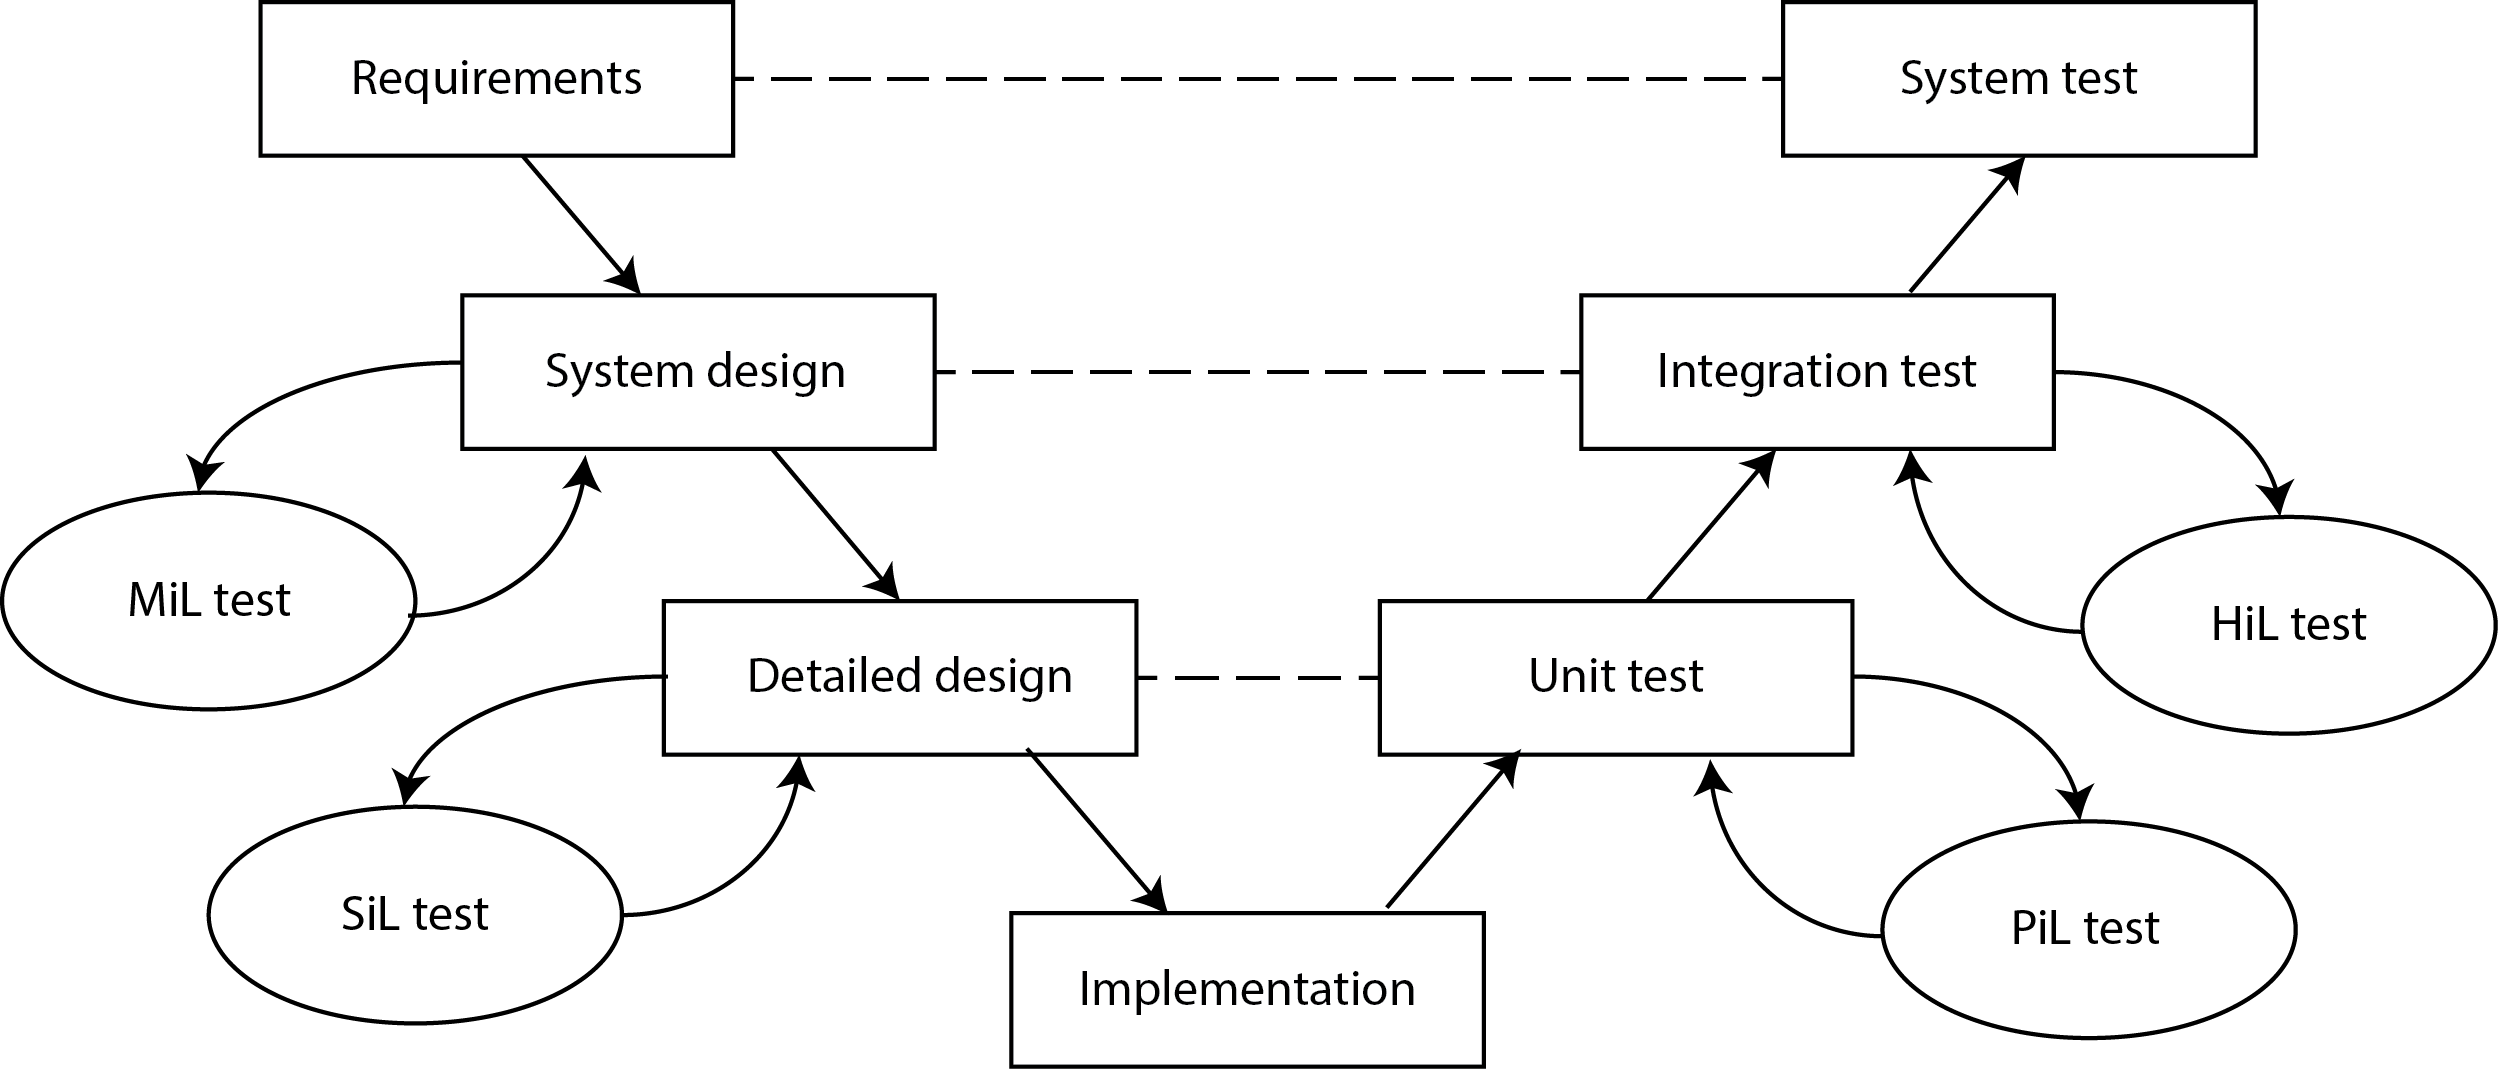
\includegraphics[width=150mm]{figures/testDesign/V_model.png}
	\caption{V-model}
	\label{fig:vModel}
\end{figure}

\subsection{V-model and testing levels}
Nowadays one of the most popular software development methodology is the V-model \cite{Vmodel} (shown on figure \ref{fig:vModel}), which defines four stages during the development and four verification steps accordingly (each step is shown with rectangles on the figure). In addition for making the development more effective for error-detection, there are four more steps defined for verifying our system's correctness, called test levels \cite{TestLevels} (shown with ellipses). While the development starts with an abstract \textbf{requirement analysis}, which declares the aim of our application, later on each step contains more detailed information. The second phase is about understanding the abstract user requirements and define the system's \textbf{functional specification} by the developers. During this phase our verification is based on \textbf{Model-in-the-Loop (MiL) testing}. The third phase contains all the low-level design and specific information about the application. From these design decisions, the \textbf{implementation} should be quite straight-forward or even it can be generated. During the \textbf{Software-in-the-Loop (SiL) testing}, the implementation will be verified for a subset of functionalities, which is depending on the system's purpose and requirements.
As of now our implementation is done and our design decisions are verified, we make sure with \textbf{unit tests} that our functions are serving their exact purposes. \textbf{Processor-in-the-Loop (PiL)} testing ensures that the computing processor at the bottom of the V-model works as expected. Then moving up in the V-model with \textbf{integration tests}, we are focusing on more abstract and complex components. In this phase we consider software and hardware elements also, completed with \textbf{Hardware-in-the-Loop (HiL)} testing. The last step is about verifying the complete system in real environment and check the high-level requirements.

\todo[inline]{give details about the used test design techniques}

\section{Test documentation}
During the test design phases of the MoDeS$^3$ I will follow a subset of the ISO 291119 standard \cite{IEEE13}.
First I will describe the documents in general, which will be later used in the MoDeS$^3$ test documentation process in section \autoref{TestDoc:MODES}. As of now the organizational and role details are irrelevant for this project, I will just give a short example for those. In the following sections, I will subtract the documentations into 3 phases, called Organizational, Test Management and Dynamic Test Documentation. 
\todo[inline]{redraw figure to something similar}
\begin{figure}[!h]
	\centering
	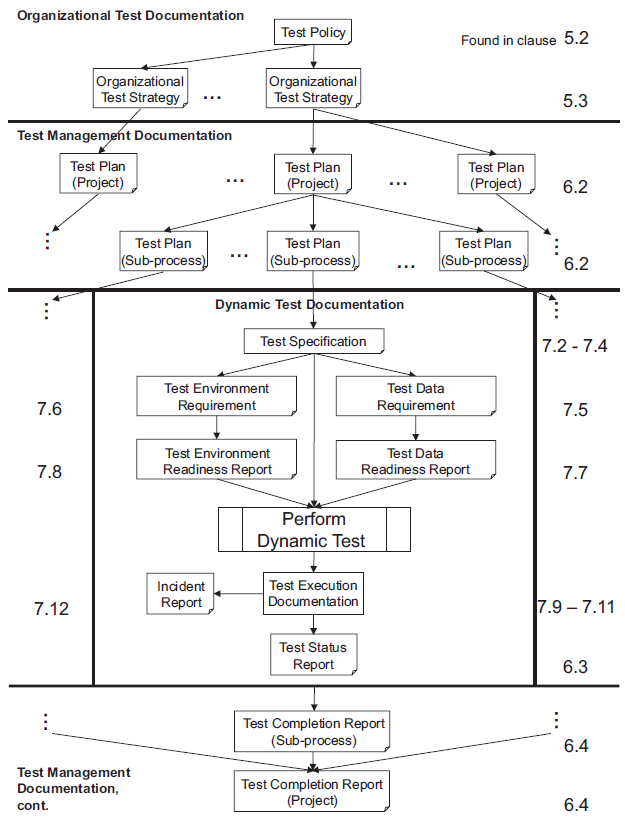
\includegraphics[width=150mm, keepaspectratio]{figures/testDesign/TestDoc.png}
	\caption{test Documentation Overview}
	\label{fig:TestDocOverview}
\end{figure}

\subsection{Organizational test documentation}
These general documents must be distributed organizational-wise and must be the same for every project within the organization. In according to this, during the test documentation the organization will be the MoDeS$^3$ team and the only project will be the above detailed railway system.

\paragraph{Test Policy}
Throughout the test development a Test Policy must contain the test principles and objectives for the whole organization. It clarifies what should be tested during development, but not how testing must be implemented. Furthermore it must define the provisions to be used for establishing, improving, maintaining and reviewing the test Policy.

\paragraph{Test Strategy}
A Test Strategy must define a proper guideline on how testing should be performed for all projects in the organization. In our case one Test Strategy is sufficient, but for an organization which have projects in different technical areas, can have a Test Strategy for each area. In latter case, the organization can define separate Test sub-processes to satisfy any special need for an area or project.

\todo[inline]{Do I need more details about test sub-processes?}

%\begin{enumerate}
%	\item Organizational Test Strategy
%	\begin{enumerate}
%		\item Introduction
%		\item General test strategy statements
%		\begin{enumerate}
%			\item Generic risk management
%			\item Test selection and prioritization
%			\item Test documentation and reporting
%			\item Test automation and tools
%			\item Configuration management of test work products
%			\item Incident management
%			\item Test sub-processes
%		\end{enumerate}
%	\end{enumerate}
%\end{enumerate}

\subsection{Test Management Documentation}
The Test Management Documentation is focusing on one project's planning and test evaluation. This group of documentation provides guidelines for Test Plan, Test Status Report and Test Completion Report.

\paragraph{Test Plan}
The collection of the test planning and test management documents is the Test Plan. It's scope be mapped to multiple projects, a single project or to sub-projects, where each Test Plan is dedicated for a sub-process (For example system test plan, integration software test plan, sub-system test plan, or unit software test plan). In a complex design structure it is advised to have a mapping tree document, which shows the relations between these Test Plans.

\paragraph{Test Status Report}
A report from the currently ongoing test process in a given reporting period is the Test Status Report. For example in an agile project it can be delivered at the end of the iteration. Although it is not necessarily a written document.

\paragraph{Test Completion Report}
As a summary of our test execution, a Test Completion Report can be provided for every test sub-process or for the whole project itself.

\subsection{Dynamic Test Documentation}
During the Dynamic Test Documentation phase the following documents are prepared:
\begin{itemize}
	\item Test Specification with sub-documents of:
	\begin{itemize}
		\item Test Design Specification
		\item Test Case Specification
		\item Test Procedure Specification
	\end{itemize}
	\item Test Data Requirements
	\item Test Environment Requirements
	\item Test Data Readiness Report
	\item Test Environment Readiness Report
	\item Test Execution Documentation with sub-documents of:
	\begin{itemize}
		\item Actual Result
		\item Test Results
		\item Test Execution Log
		\item Incident Report
	\end{itemize}
\end{itemize}
\todo[inline]{Figure of test docs hierarchy can be added here}

In the following sections, I will give a brief summary for each documentation.

\paragraph{Test Design Specification} \label{TestDoc:TDS}
The features and test conditions (derived from test basis) are collected in the Test Design Specification with the specific test cases and test procedures. These detailed test cases will be executed during testing process. 

Here we can create groups called \textit{feature sets} for those features which are connected together, then we can handle them independently.  A \textit{test condition} is aligned for each feature set and can be verified by a test case. Technically a test condition means a concrete state or representation of a feature. In addition on or more requirement can be referenced by a test case. In addition, to develop a more maintainable test document we must take care for the references from test cases to each requirement.

\paragraph{Test Case Specification}
One or more feature set with the defined test conditions and coverage items, constitutes a Test Case Specification.

\textit{Test coverage items} are obtained from a set of test conditions and specific test design technique. These items can be summarized in a list (describing test coverage items, test conditions and feature sets with proper priorities). From each test coverage item a \textit{Test case} can be derived, which verifies the correct implementation of a function. Regarding the possible number of test cases it can be collected into a list, table or database. Each test case should have a proper definition of dependencies. These are collected in \autoref{table:TestDoc:TestCases}.

\begin{table}[h]
	\caption{Details of a test case}
	\label{table:TestDoc:TestCases}
	\begin{center}
		\renewcommand{\arraystretch}{1.8}
		\begin{tabu} 
			to 0.9 \textwidth
			{  X[c]  X[c] }
			\toprule
			Aspect                     & Description                                                                                                                                               \\ \midrule
			Priority                   & Defines the execution order and importance between test cases. Higher priority test cases should be examined earlier then lower priorities                \\
			Traceability               & Reference the parent test coverage, condition item and the feature requirement                                                                            \\
			Preconditions              & Describes special states that must exists to execute the test case (Can be other test cases also)                                                         \\
			Inputs                     & A specific action which sets the test item into a state, where the actual and expected results can be compared                                            \\
			Expected result            & Specifies the expected output and behavior (with tolerances) of the test item which was in the precondition state and was modified with the proper inputs \\
			Actual result, test result & A description of test item outputs and a comparison between actual and expected results                                                                   \\ \bottomrule
		\end{tabu}
	\end{center}
\end{table} 

\paragraph{Test Procedure Specification}
Describes the precondition setup and test cases execution in the proper order with possible post evaluation activities.

Those test cases, which have the same purpose in the test item's property (for example precondition, test basis or even in the identified risk) can be collected into a \textit{Test set}. Typically this will reflect to one or more feature sets. For each \textit{Test set} the proper execution order is defined in the \textit{Test procedure} considering test case dependencies, preconditions, postconditions and other environment requirements.

\paragraph{Test Data Requirements}
Defines the required properties of the test data, which is used during test procedure execution. These requirements can be summarized with a list. In addition, this detailed test data requirements makes it more maintainable and traceable. 

\paragraph{Test Data Readiness Report} 
Gives a list of Test Data Requirements determining whether they are satisfied or not.

\paragraph{Test Environment Requirements}
Describes the required test environment properties, which are setting the test items into the expected test environment. These requirements can also be grouped by environment types like hardware, middleware, software, tools or security and may vary for each test case.

\paragraph{Test Environment Readiness Report}
Lists the fulfillment of Test Environment Requirements.

\paragraph{Actual Results}
After executing the selected test procedures, each test case's actual result (output state or behavior after the input actions) should be recorded. It may require full recording of the process with an automated tool also.

\paragraph{Test Result}
Determines if the actual results are corresponding to the expected results with the specified deviation or not. It is usually recorded as passed or failed, along with the actual results.

\paragraph{Test Execution Log}
Detailed documentation of one or more test procedure's execution. Can be represented in a list or table with measuring times and events of the test execution.

\paragraph{Test Incident Reporting}
If there is any deviation between the actual and expected results after each test procedure execution, we should create a dedicated Incident Report detailing the problems. These reports could contain a description of the problem with severity, date and possible risk information.

%----------------------------------------------------------------------------
\chapter{Test Planning for MoDeS$^3$ project}\label{TestDoc:MODES}
%----------------------------------------------------------------------------

\section{Test Policy for MoDeS$^3$ organization}
\paragraph{Scope:} The following Test Policy must be followed by the MoDeS$^3$ team in the Department of Measurement and Information Systems.
\paragraph{Introduction:} The railway system project have started several years back, and from time to time the team faced smaller and bigger problems with the implemented product. Presumably a high percentage of them could be prevented with a detailed test documentation and process. To avoid these situations in the future I will now introduce a test documentation approach for the demonstrator railway system.
\paragraph{Objectives of testing:} The objective of testing is to measure and improve the software quality and to avoid safety-critical failures in the system.
\paragraph{Standards:} This test documentation will follow the ISO/IEC/IEEE standard 291119-3 "Test Documentation" part \cite{IEEE13}.
\paragraph{Test improvement:} Every student or a group of them who participated in the test implementation should give an overview about the test results and their execution aligned with the test documentation approach. Any further developed component should be covered by test cases with the corresponding test documentation. Consequently the requirements, the test plan sub-processes (unit, integration and system test plans) and the design specifications must be extended to cover the newly attached or modified components.
\paragraph{Test evaluation:} Each extension should be handled as a github pull request, which must be reviewed by 2 of the team members and additionally must be checked by the student's supervisor.

\section{Test Strategy for MoDeS$^3$ projects}
\paragraph{Scope:} The following test strategy is applicable for the demonstrator railway system project (described in \autoref{chapter:RailwaySystem}). This strategy's aim is to support testing implementation and maintainability at the software development phases in component, integration and system level also.
\paragraph{Risk management:} A risk management must be handled for test plans separately. The detailed format must be a traceable list or table.
\paragraph{Test selection prioritization:} The test cases and test procedures will follow a bottom-up strategy order, aligned with safety-critical risk levels. Consequently a test element with lower dependencies and more independent functionalities (also more hardware related) got higher priority than a complex test element, which relies on multiple sub components.
\paragraph{Test document and reporting:} The test process and documentation must be well-separated and clear that a new team member can easily understand the structure.
\paragraph{Test automation and tools:} All tools, which is used during the test process and documentation must be available for a university student (meaning education license or freeware).
\paragraph{Incident management:} All detected defects must be created as a github issue. \footnote{MoDeS$^3$ github page is available at the following page: \url{https://github.com/FTSRG/BME-MODES3}}
\paragraph{Test sub-processes:} All test projects must provide the following test levels: unit test plan, integration test plan, system test plan.

\section{Master Test Plan for Railway System project}\label{section:MTP}
\paragraph{Scope:} Test plan's scope is to provide the necessary test framework for executing tests for the demonstrator railway system of MoDeS$^3$ team. This document identifies a way for planning, executing and maintaining tests in a multi-layered project.
\paragraph{Plan context:} The railway system architecture (detailed in \autoref{chapter:RailwaySystem}) consist of off-the-shelf and custom hardware and software elements. According to this, the \textit{test items} are only the custom software elements, which were made by the MoDeS$^3$ team. Details about test items can be found in \autoref{section:CustomSW}. Other product testing and the custom hardware extension verifications are not part of this Test Documentation. Furthermore not all the software component have been involved in this testing plan, because not safety-critical components have been skipped. \textit{Barrier} is irrelevant regarding the train-collision detection. An additional way to set the speed and directions of the trains is not safety-critical either, so \textit{LeapMotion} and \textit{XPressNet} components are not safety-critical (Note that an other components are capable to detect train positions on the railway). \textit{Touchboard} is a component which have a reduced functionality considered to \textit{Dashboard}, so we will skip that also in this test plan.
\paragraph{Risk register:} On the following 2 tables the possible product (\autoref{table:Product-risks}) and project risks (\autoref{table:Project-risks}) are described. The following assessment will cover the risk management for all the test sub-plans in the MoDeS$^3$ project.

\begin{table}[!h]
\caption{Product risks}
\label{table:Product-risks}
	\begin{center}
		\renewcommand{\arraystretch}{1.8}
		\begin{tabu} 
			to 0.9 \textwidth
			{ X[0.1, c] X[0.5, l] X[l] X[0.4, l] }
			\toprule
			ID & Risk details                            & Mitigation activities                                                                  & Level        \\ \midrule
			                                                      \multicolumn{4}{c}{Occupancy detection}                                                        \\
			1  & Wrong or no occupancy detected          & Review of appropriate hardware and software elements considering network connection    & High         \\
			                                                   \multicolumn{4}{c}{Track element controlling}                                                     \\
			2  & Not controllable turnout or segment     & Review of hardware and software components considering standard railway elements also. & Above middle \\
			                                                  \multicolumn{4}{c}{Safety critical verification}                                                   \\
			3  & Wrong collision avoidance decision made & Review of design and safety algorithm. Extra test cases to cover incorrect scenarios   & High         \\
			4  & Train collision                         & Review of design and safety algorithm.                                                 & High         \\ \bottomrule
		\end{tabu}
	\end{center}
\end{table}

\begin{table}[!h]
	\caption{Project risks}
	\label{table:Project-risks}
	\begin{center}
		\renewcommand{\arraystretch}{1.8}
		\begin{tabu} 
			to 0.9 \textwidth
			{ X[0.1, c] X[0.5, l] X[l] X[0.4, l] }
			\toprule
			ID & Risk                         & Mitigation activities                                                                                                                                                                                             & Level  \\ \midrule
			1  & Busy students and estimation & For a student every semester is different and not always predictable how much time will the student have for the project. Therefore it must be consider during project estimation and planning accordingly.       & Middle \\
			2  & New students and planning    & This is a university project, so we must calculate with the often changing student and knowledge transfer about the existing system.                                                                              & High   \\
			3  & Cutting-edge tools           & Unpredictable cutting-edge technologies can make a huge rule during project planning. The compatibility of tools and their reliability can differ during few month also, which must be adapted during estimation. & Above middle   \\ \bottomrule
		\end{tabu}
	\end{center}
\end{table}

\paragraph{Test strategy:} 
For the railway system project, the following test sub-processes are defined:
\begin{itemize}
	\item Unit test (see in \autoref{ssection:UTP})
	\item Integration test (see in \autoref{ssection:ITP})
	\item System test (see in \autoref{ssection:STP})
\end{itemize}
In addition for all sub-processes the following documents must be delivered:
\begin{itemize}
	\item Test sub-process plan
	\item Test specification
	\item Test log
	\item Test sub-process completion or status report
\end{itemize}
The test design techniques, test completion criteria and test data must be applied accordingly for every test sub-process. We use the following test environments in general for every test sub-process:
\begin{itemize}
	\item Eclipse Photon where applicable
	\item Visual Studio Code where applicable
	\item JUnit Jupiter for Java base components and GoogleTest for components written in C++
	\item Mockito with PowerMockito for components written in Java
\end{itemize}
\paragraph{Test activities and estimates:} These are confirmed personally and aligned with university studies.
\paragraph{Stuffing:} The actual team and roles are highly dependent with the MoDeS$^3$ team in every semester.
\paragraph{Retesting and regression testing:} This is specified for each test sub-process.

\subsection{Unit Test Plan}\label{ssection:UTP}
\paragraph{Scope:} The aim for this Test Plan is to verify each software component's functionality in the system. This plan is derived from a Master Test Plan (detailed the \autoref{section:MTP} for Master Test Plan). 
\paragraph{Plan context:} Unit Test Plan context is the same as for Master Test Plan (see \autoref{section:MTP}), because all self developed software component must be tested in a standalone environment also. 
\paragraph{Risk register:} Same as Master Test Plan.
\paragraph{Test strategy:} The deliverables are this test plan, the unit test specification and the test status report. For every software component the code coverage measurement must reach at least 80\%. This means that for each component the implemented unit tests must execute greater or equal then 80\% of the component's code.

\subsection{Integration Test Plan}\label{ssection:ITP}
\paragraph{Scope:} This test plan is stands for the integration level testing examination. This approach is one abstraction layer above from the unit tests, because the following test cases verifies the correct functionalities between one or more components. This test plan is also derived from a Master Test Plan (detailed the \autoref{section:MTP} for Master Test Plan).
\paragraph{Plan context:} In this plan we aim to test the system divided into several groups, consequently the Integration Test Plan's context is the same as for Master Test Plan (see \autoref{section:MTP}) and for Unit Test Plan.
\paragraph{Risk register:} Same as Master Test Plan.
\paragraph{Test strategy:} The deliverables are this test plan, the integration test specification and the test status report. It is required to cover every existing connection between 2 components with at least 1 parameter of a message type. (Component communication is described in \autoref{fig:communicationModel}.)

\subsection{System Test Plan}\label{ssection:STP}
\paragraph{Scope:} The third test plan is designed to test the demonstrator functions at system level. These tests are verifies the system's commonly demonstrated features. This test plan is also derived from a Master Test Plan (detailed the \autoref{section:MTP} for Master Test Plan). 
\paragraph{Plan context:} This plan's focus is the whole railway system, therefore the context is the same as for Master Test Plan (see \autoref{section:MTP}).
\paragraph{Risk register:} Same as Master Test Plan.
\paragraph{Test strategy:} The deliverables are this test plan, the system test specification and the test status report. The test cases must cover the safety-critical functionalities (see details in \autoref{section:SC-Functionalities}) of the demonstrator system and greater than 50\% of the system requirements (described in \autoref{section:REQ}) for every component.

\section{Test Design Specification for Unit Test Plan}

\paragraph{Purpose:} The purpose of this test specification is to give a guideline for executing unit tests for the demonstrator railway system components.
\paragraph{References:} The railway system related requirements can be found in \autoref{section:REQ}.

\subsection{Feature Sets} We can easily separate the system's functionalities into feature sets following the referenced system requirement's structure, which are shown in \autoref{table:Feature-Sets-Unit}.
\begin{table}[H]
\caption{Feature sets}
\label{table:Feature-Sets-Unit}
	\begin{center}
		\renewcommand{\arraystretch}{1.8}
		\begin{tabu} 
			to 1.0 \textwidth
			{  X[0.7, c] X[2.0, c] X[3.0, c] X[0.5,c] X[2.0, c] X[2.0, c] }
			\toprule
			\multicolumn{2}{c}{Feature Set} & Scope                                                                                             & Priority & Approach                                             & Traceability                                                                   \\ \midrule
			ID   & Name                     &                                                                                                   &          &                                                      &                                                                                \\ \midrule
			FS-1 & GPIO handling            & To test GPIO pin handling                                                                         & Am       & Scenario Testing with Equivalence Class Partitioning & \ref{req:GPIO-1}, \ref{req:GPIO-2}                                             \\
			FS-2 & Occupancy detection      & To test the occupancy related functionalities in the system, including state and change detection & H        & Decision Table Testing                               & \ref{req:OCQ-1}, \ref{req:OCQ-2}, \ref{req:SOQ}                                \\
			FS-3 & Track element controller & To test segment availability and turnout direction setting                                        & Am       & Scenario Testing                                     & \ref{req:TEC-1}, \ref{req:TEC-2}                                               \\
			FS-4 & Safety Logic             & To test railway system's safety logic                                                             & H        & Scenario Testing                                     & \ref{req:SL-1}, \ref{req:SL-2} , \ref{req:SL-3}, \ref{req:SL-4}                \\
			FS-5 & Dashboard                & To test Dashboard capabilities                                                                    & L        & Scenario Testing                                     & \ref{req:DB-1}, \ref{req:DB-2}, \ref{req:DB-3}, \ref{req:DB-4}, \ref{req:DB-5} \\ \bottomrule
		\end{tabu}
	\end{center}
\end{table} 

\subsection{Test Conditions} In the following section I will describe the test conditions for each feature set. Most of the feature sets in the Unit Test Plan are simple low level functions so the test conditions also will describe the test coverage items.

\paragraph{GPIO handling (FS-1)}
Considering the GPIO's functionality the following test conditions are test coverage items also. With the usage of use case based design approach, the GPIO can be used for input and output communication. The proper setup and operation cases are detailed in  \autoref{table:TC-FS-1}.
\begin{table}[H]
	\caption{GPIO handling test condition and coverage items}
	\label{table:TC-FS-1}
	\begin{center}
		\renewcommand{\arraystretch}{1.8}
		\begin{tabu} 
			to 0.9 \textwidth
			{  X[c] X[c] X[c] X[c] X[c] }
			\toprule
			Test condition & Direction                     & Phase                            & Configuration file           & Setting \\ \midrule
			FS-1/1.0       & \centeredDoubleRow{3}{Input}  & Initialization                   & edge                         & both    \\
			FS-1/1.1       &                               & \centeredDoubleRow{2}{Operation} & \centeredDoubleRow{2}{value} & low     \\
			FS-1/1.2       &                               &                                  &                              & high    \\
			FS-1/2.0       & \centeredDoubleRow{2}{Output} & Initialization                   & \centeredDoubleRow{3}{value} & low     \\
			FS-1/2.1       &                               & \centeredDoubleRow{2}{Operation} &                              & low     \\
			FS-1/2.2       &                               &                                  &                              & high    \\ \bottomrule
		\end{tabu}
	\end{center}
\end{table} 

\paragraph{Occupancy detection (FS-2)}
The 2 test condition items are also considered as test coverage items, which are shown in \autoref{table:TC-FS-2}). The detection is made periodically in the demonstrator system life-cycle and the decision can be that the section is either free or occupied.
\begin{table}[H]
	\caption{Occupancy detection test condition and coverage items}
	\label{table:TC-FS-2}
	\begin{center}
		\renewcommand{\arraystretch}{1.8}
		\begin{tabu} 
			to 0.9 \textwidth
			{  X[c] X[c] X[c] }
			\toprule
			Test condition & Value    & Comment             \\ \midrule
			FS-2/1.0       & Free     & Specific segment is free     \\
			FS-2/1.1       & Occupied & Specific segment is occupied \\ \bottomrule
		\end{tabu}
	\end{center}
\end{table}


\paragraph{Track element controller (FS-3)}
A track element controller can handle segment and turnout specific statements also, consequently we must distinguish our test condition and coverage items for these segment types. The merged test condition and coverage items are shown in \autoref{table:TC-FS-3}. The specific use cases for a segment, that it can be enabled or disabled by the controller whether a train can drive on it or not. Consequently the use case for the turnout to change its state between straight and divergent.
\begin{table}[H]
	\caption{Track element controller test condition and coverage items}
	\label{table:TC-FS-3}
	\begin{center}
		\renewcommand{\arraystretch}{1.8}
		\begin{tabu} 
			to 0.9 \textwidth
			{  X[c] X[c] X[c] }
			\toprule
			Test condition & Affected element               & State     \\ \midrule
			FS-3/1.0       & \centeredDoubleRow{2}{Segment} & Enabled   \\
			FS-3/1.1       &                                & Disabled  \\
			FS-3/2.0       & \centeredDoubleRow{2}{Turnout} & Straight  \\
			FS-3/2.1       &                                & Divergent \\ \bottomrule
		\end{tabu}
	\end{center}
\end{table} 

\paragraph{Safety Logic (FS-4)}
The safety-critical aspects are shown in \autoref{table:TC-FS-4}, which should be handled by the Safety Logic.
\begin{table}[H]
	\caption{Safety Logic test condition items}
	\label{table:TC-FS-4}
	\begin{center}
		\renewcommand{\arraystretch}{1.8}
		\begin{tabu} 
			to 0.9 \textwidth
			{  X[c] X[c] X[c] }
			\toprule
			Test condition & Safety Level                  & Safety type     \\ \midrule
			FS-4/1.0       & \centeredDoubleRow{2}{System} & Train collision \\
			FS-4/2.0       &                               & Turnout derail  \\ \bottomrule
		\end{tabu}
	\end{center}
\end{table} 

\paragraph{Dashboard (FS-5)}
A full use case coverage is aimed for the Dashboard which can be defined by the following test condition and coverage items, shown in \autoref{table:TC-FS-5}.
\begin{table}[H]
	\caption{Dashboard test conditions}
	\label{table:TC-FS-5}
	\begin{center}
		\renewcommand{\arraystretch}{1.8}
		\begin{tabu} 
			to 0.9 \textwidth
			{  X[c] X[c] X[c] X[c] }
			\toprule
			Test condition & Scope                       & Section type                   & State     \\ \midrule
			FS-5/1.0       & \centeredDoubleRow{4}{All}  & \centeredDoubleRow{2}{Turnout} & Straight  \\
			FS-5/1.1       &                             &                                & Divergent \\
			FS-5/1.2       &                             & \centeredDoubleRow{2}{Segment} & Enabled   \\
			FS-5/1.3       &                             &                                & Disabled  \\
			FS-5/2.0       & \centeredDoubleRow{4}{Each} & \centeredDoubleRow{2}{Turnout} & Straight  \\
			FS-5/2.1       &                             &                                & Divergent \\
			FS-5/2.2       &                             & \centeredDoubleRow{2}{Segment} & Enabled   \\
			FS-5/2.3       &                             &                                & Disabled  \\ \bottomrule
		\end{tabu}
	\end{center}
\end{table} 

\subsection{Test coverage items}
\paragraph{Safety Logic: Train collision test coverage items (FS-4/1.0)}
\begin{enumerate}[label=FS-5/1.0-\arabic*, leftmargin=*, format=\small]
	\item 1 Train is moving to a segment where there is an other train
	\item 1 Train is moving to a segment where the other train is in 1 distance away on any the path
	\item 1 Train is moving to a segment where the other train is in 2 distance away on any the path
\end{enumerate}
\paragraph{Safety Logic: Turnout derail test coverage items (FS-4/2.0)}
\begin{enumerate}[label=FS-5/2.0-\arabic*, leftmargin=*, format=\small]
	\item Train is moving through a turnout from top to divergent, while the turnout is in straight state
	\item Train is moving through a turnout from top to straight, while the turnout is in divergent state
\end{enumerate}

\subsection{Test cases}\label{section:UnitTestCases}
In this section I will describe the test cases defined by test conditions and coverage items for each feature set. In addition for all the feature sets just one test case will be mentioned and additional test cases can be found in the \ref{appendix:UnitTC} appendix.
\paragraph{Gpio Handling (FS-1) test cases} In order to work in production with GPIO component, the following configuration file must exists: sys/gpio/gpioPIN/export, sys/gpio/gpioPIN/value and sys/gpio/gpioPIN/edge. This need is also propagate to all test cases regarding GPIO handling, so files must be accessible or mocked. 
\begin{table}[H]
	\caption{Test case 1-1}
	\label{table:TCase-FS1-01}
	\begin{center}
		\renewcommand{\arraystretch}{1.8}
		\begin{tabu} 
			to 0.9 \textwidth
			{  X[0.3, l] X[l] }
			\toprule
			Test case ID: 1-1 & Purpose: to test the GPIO initialization in input direction. \newline Priority: am \newline Tracing: FS-1/1.0 \\ \midrule
			Precondition      & The GPIO's necessary files are available.                                                                     \\
			Input             & Initialize the GPIO itself with input direction.                                                              \\
			Expected result   & The "both" string have been written to "edge" configuration file.                                             \\ \bottomrule
		\end{tabu}
	\end{center}
\end{table}

\paragraph{Occupancy detection (FS-2) test cases} Occupancy detection components cannot be easily separated into subcomponents for testing purpose, because the communication between their parts is based on a serial port connection. There is no fake serial port connection available on the market for windows operating system, so we must test them together with real hardware connection or modify our implementation.

\begin{table}[H]
	\caption{Test case 2-1}
	\label{table:TCase-FS2-01}
	\begin{center}
		\renewcommand{\arraystretch}{1.8}
		\begin{tabu} 
			to 0.9 \textwidth
			{  X[0.3, l] X[l] }
			\toprule
			Test case ID: 2-1 & Purpose: to test the detection of segment occupancy (the train power consumption) through section occupancy query, when the specific segment is free\newline Priority: above middle \newline Tracing: (FS-2/1.0) \\ \midrule
			Precondition      & S88 serial port connection and available Arduino hardware element                                                                                                                                                \\
			Input             & Unclosed circuit between the specific segment's hardware elements elements                                                                                                                                       \\
			Expected result   & Occupancy components have queried free occupancy state                                                                                                                                                           \\ \bottomrule
		\end{tabu}
	\end{center}
\end{table} 

\paragraph{Track element controller (FS-3)  test cases} This component can further be divided into segment and turnout controllers like on hardware level. Although in this test plan, it does not detailed into further test cases for the specific controllers, because in software point of view, there is no need to distinguish them.

\begin{table}[H]
	\caption{Test case 3-1}
	\label{table:TCase-FS3-01}
	\begin{center}
		\renewcommand{\arraystretch}{1.8}
		\begin{tabu} 
			to 0.9 \textwidth
			{  X[0.3, l] X[l] }
			\toprule
			Test case ID: 3-1 & Purpose: to test the track element controller's segment state setting as enabled \newline Priority: above middle \newline Tracing: (FS-3/1.0) \\ \midrule
			Precondition      & Observable GPIO components                                                                                                                    \\
			Input             & Call the track element controller set segment state function with enabled parameter                                                           \\
			Expected result   & All GPIO levels are in "HIGH" state, which are related to the specific segment                                                                \\ \bottomrule
		\end{tabu}
	\end{center}
\end{table}

\paragraph{Safety logic (FS-4) test cases} The following test cases are related to system level safety logic feature set.
\begin{table}[H]
	\caption{Test case 4-1}
	\label{table:TCase-FS4-01}
	\begin{center}
		\renewcommand{\arraystretch}{1.8}
		\begin{tabu} 
			to 0.9 \textwidth
			{  X[0.3, l] X[l] }
			\toprule
			Test case ID: 4-1 & Purpose: to test the safety logic awareness, when a train is moving on a path where the next section in the direction already occupied by an other train \newline Priority: high \newline Tracing: (FS-4/1.0) \\ \midrule
			Precondition      & None                                                                                                                                                                                                          \\
			Input             & Insert a train to a specific segment and move an other train to the adjacent segment                                                                                                                          \\
			Expected result   & Safety Logic sent a segment disable command with the id of the specific segment                                                                                                                               \\ \bottomrule
		\end{tabu}
	\end{center}
\end{table} 

\paragraph{Dashboard (FS-5) test cases} The following test cases are Dashboard feature set related items. This component can control and visualize the current track element states, consequently the unit test cases are checking the control network messages.
\begin{table}[H]
	\caption{Test case 5-1}
	\label{table:TCase-FS5-01}
	\begin{center}
		\renewcommand{\arraystretch}{1.8}
		\begin{tabu} 
			to 0.9 \textwidth
			{  X[0.3, l] X[l] }
			\toprule
			Test case ID: 5-1 & Purpose: to test the dashboard's set all turnout to straight functionality  \newline Priority: am \newline Tracing: FS-5/1.0 \\ \midrule
			Precondition      & All turnout must be in divergent state                                                                                       \\
			Input             & Simulate a button press to the change all turnout direction function                                                         \\
			Expected result   & Message have been prepared to send with straight and a turnout id parameter for all turnouts                                 \\ \bottomrule
		\end{tabu}
	\end{center}
\end{table}

\subsection{Test Procedure Specification}
In this Unit Test Plan, each feature set is derived from a custom software component in the demonstrator railway system. Regarding this property each test set can involve a group of test cases which are related for that feature set. A unit test must be a fast, isolated, repeatable, self-validated execution, therefore test set's ordering should not influence the test results. Consequently we can execute them independently and parallel but we can also give an order, for example as the test cases ordered in the Test case definition section (described in \autoref{section:UnitTestCases}) and one test procedure can contain one test set. 

\section{Test Design Specification for Integration Test Plan}

\paragraph{Purpose:} The aim of the following test specification is to give instructions about setting up and executing integration tests. These tests will verify two or more component's behavior together.
\paragraph{References:} The railway system related requirements can be found in \autoref{section:REQ}.

\subsection{Feature Sets} 
In the (\ref{table:Feature-Sets-integration}) table the components of the demonstrator railway system are grouped into integration feature sets separated by functional purposes.
\begin{table}[H]
	\caption{Feature sets for Integration Test Plan}
	\label{table:Feature-Sets-integration}
	\begin{center}
		\renewcommand{\arraystretch}{1.8}
		\begin{tabu} 
			to 1.0 \textwidth
			{  X[0.7,c] X[1.5, c] X[3.0, c] X[0.7,c] X[c] X[2.0,c] }
			\toprule
			       \multicolumn{2}{c}{Feature Set}        & Scope                                                                                                        & Priority & Approach         & Traceability                                                      \\ \midrule
			ID    & Name                                  &                                                                                                              &          &                  &                                                                   \\ \midrule
			FSI-1 & Occupancy message                     & To test the occupancy network messages sent out by the occupancy components                                  & Am       & Scenario Testing & \ref{req:OCQ-1}, \ref{req:OCQ-2}, \ref{req:SOQ}                   \\
			FSI-2 & Track element controller instructions & To test Track element controller and GPIO handling functionalities, manipulating by network command messages & Am       & Scenario Testing & \ref{req:TEC-1} \ref{req:TEC-2} \ref{req:GPIO-1} \ref{req:GPIO-2} \\ \bottomrule
		\end{tabu}
	\end{center}
\end{table} 

\subsection{Test Conditions and coverage items}
The test condition and coverage items for the integration tests can be defined with the same aspects as the specific component in the unit test plan.
The following enumeration is showing a mapping between the integration and unit test feature sets.
\begin{enumerate}
	\item Occupancy message (FSI-1) - Occupancy detection (FS-3) (\ref{table:TC-FS-2})
	\item Track element controller instructions (FSI-2) - Track element controller(\ref{table:TC-FS-3})
	\item Safety Logic interaction (FSI-3) - Occupancy detection (FS-3) (\ref{table:TC-FS-2})
	\item Safety logic intervention (FSI-4) - Safety Logic (FS-4) (\ref{table:TC-FS-4})
\end{enumerate}

\subsection{Test cases}
The following test cases are a subset of all integration test cases, which are fully detail in \autoref{appendix:IntTC}.
\paragraph{Occupancy message (FSI-1) text cases} The occupancy related test cases are verifying the network message sent by the Occupancy Query software element.
\begin{table}[H]
	\caption{Integration test case 1-1}
	\label{table:TCase-FSI1-01}
	\begin{center}
		\renewcommand{\arraystretch}{1.8}
		\begin{tabu} 
			to 0.9 \textwidth
			{  X[0.3, l] X[l] }
			\toprule
			Integration test case ID: 1-1 & Purpose: to test the detection of segment occupancy when a segment is free and to verify the propagated network occupancy message \newline Priority: am \newline Tracing: FS-2/1.0 \\ \midrule
			Precondition                  & There must be an MQTT server connection available and an connected with serial port                                                                                                \\
			Input                         & Unclosed circuit between the specific segment's hardware elements                                                                                                                  \\
			Expected result               & A new segment occupancy message must be send to the network with free segment state  and the specific segment id                                                                   \\ \bottomrule
		\end{tabu}
	\end{center}
\end{table} 


\paragraph{Track element controller instructions (FSI-2) test cases}\label{p:TEC-ITC} The main focus in the following test cases is to send segment and turnout command messages to the Track element controller. We can further observer the file output for the supervised GPIOs.
\begin{table}[H]
	\caption{Integration test case 2-1}
	\label{table:TCase-FSI2-01}
	\begin{center}
		\renewcommand{\arraystretch}{1.8}
		\begin{tabu} 
			to 0.9 \textwidth
			{  X[0.3, l] X[l] }
			\toprule
			Integration test case ID: 2-1 & Purpose: to test the track element controller, that it enables its supervised segment's state \newline Priority: am \newline Tracing: FS-3/1.0 \\ \midrule
			Precondition                  & There must be an MQTT server connection available                                                                                              \\
			Input                         & Send a SegmentCommand message with enabled state and a segment id which is supervised by the track element controller component                \\
			Expected result               & All related GPIO (pru and app) has the writer with value "1" and targetFile "value"                                                            \\ \bottomrule
		\end{tabu}
	\end{center}
\end{table} 
\subsection{Test procedure} 
In the integration test plan all the FSI-1 feature set related test cases requires hardware components during test execution. Apart from that all other test cases are purely software component tests, therefore they can be executed separately.

\section{Test Design Specification for System Test Plan}

\paragraph{Purpose:} The system test plan is describes a road map to verify the high-level requirements of the railway system.
\paragraph{References:} The related requirements are previously described in \autoref{section:REQ}.

\subsection{Feature Sets} 
%1) manual with dashboard: check segments and turnouts
%2) SL checks: change turnout so trains can collide, change turnout and cut it with a train

\begin{table}[!h]
	\caption{System feature sets}
	\label{table:Feature-Sets-System}
	\begin{center}
		\renewcommand{\arraystretch}{1.8}
		\begin{tabu} 
			to 1.0 \textwidth
			{  X[0.8, c] X[1.5, c] X[3.0, c] X[0.7,c] X[c] X[2.0,c] }
			\toprule
			        \multicolumn{2}{c}{Feature Set}         & Scope                                                        & Priority & Approach            & Traceability                                                               \\ \midrule
			ID    & Name                                    &                                                              &          &                     &                                                                            \\ \midrule
			FSS-1 & Track element availability verification & To test the railway system track element's proper operations & Am       & Scenario Testing & \ref{req:DB-1} \ref{req:DB-2} \ref{req:DB-3} \ref{req:DB-4} \ref{req:DB-5} \\
			FSS-2 & Safety logic verification               & To test the safety logic functionalities                     & H        & Scenario Testing & \ref{req:SL-1} \ref{req:SL-2} \ref{req:SL-3} \ref{req:SL-4}                \\ \bottomrule
		\end{tabu}
	\end{center}
\end{table} 

\subsection{Test condition and coverage items}
From the previously described (\ref{table:Feature-Sets-System}) feature sets the test condition and coverage items can be derived, which are detailed in the following sections.
\paragraph{Track element availability verification (FSS-1)} The purpose of this test condition is to verify that all segments and turnouts are available with a fast functional test. 
\begin{table}[H]
	\caption{Train detection test conditions}
	\label{table:TC-FSS-1}
	\begin{center}
		\renewcommand{\arraystretch}{1.8}
		\begin{tabu} 
			to 0.9 \textwidth
			{  X[c] X[c] X[c] }
			\toprule
			Test condition & Scope                      & Section type \\ \midrule
			FSS-1/1        & \centeredDoubleRow{2}{All} & Turnout      \\
			FSS-1/2        &                            & Segment      \\ \bottomrule
		\end{tabu}
	\end{center}
\end{table}
\paragraph{Safety logic verification (FSS-2)} The system level \textit{safety logic verification} the test conditions are the same as it was previously shown for unit tests in \autoref{table:TC-FS-4}. To summarize that, the conditions can be divided into turnout derail and train collision scenarios.

\subsection{Test cases} All test cases details can be found in \autoref{appendix:SystemTC}.
\paragraph{Track element availability verification (FSS-1)} The following test cases will use network segment and turnout command messages as previously described in \autoref{p:TEC-ITC} integration test case. 
\begin{table}[H]
	\caption{System test case 1-1}
	\label{table:TCase-FSS1-01}
	\begin{center}
		\renewcommand{\arraystretch}{1.8}
		\begin{tabu} 
			to 0.9 \textwidth
			{  X[0.3, l] X[l] }
			\toprule
			System test case ID: 1-1 & Purpose: to test all turnout controllability     \newline Priority: am \newline Tracing: FS-6/1.0                                \\ \midrule
			Precondition                                                              & None                                                                            \\
			Input                                                                     & Send a switch turnout command to all turnouts twice                                \\
			Expected result                                                           & All turnout state have been changed to straight from divergent and the other way \\ \bottomrule
		\end{tabu}
	\end{center}
\end{table}


\paragraph{Safety logic verification (FSS-2)} The below detailed safety logic test cases instead of checking the whole table, will just verify the safety logic decisions in the most problematic scenarios.
\begin{table}[H]
	\caption{System test case 2-1}
	\label{table:TCase-FSS2-01}
	\begin{center}
		\renewcommand{\arraystretch}{1.8}
		\begin{tabu} 
			to 0.9 \textwidth
			{  X[0.3, l] X[l] }
			\toprule
			System test case ID: 2-1 & Purpose: to test the safety logic for turnout derail scenario  \newline Priority: am \newline Tracing: FS-6/1.2 \\ \midrule
			Precondition             & Turnout T5, T1 is in straight state and a train is on the segment S13                                           \\
			Input                    & Move the train to segment S15 from segment S13 through the path of S13, S8, T5, S11, T1, S15.                   \\
			Expected result          & Before T1 turnout S11 segment is disabled by the safety logic to avoid turnout derail                           \\ \bottomrule
		\end{tabu}
	\end{center}
\end{table}

\subsection{Test procedure}
%1) STC 1-1, 1-2, 1-3
%2) STC 2-1, 2-2
\paragraph{System test procedure for FSS-1} The following procedure is focusing on verifying the track element controller functionalities. 
\begin{enumerate}
	\item Objective: FSS-1
	\item Priority: high
	\item Start up: all the track element controllers should be started properly
	\item Stop and wrap up: all track element controllers on the components must be stopped
\end{enumerate}
\begin{table}[H]
	\caption{System test procedure for FSS-1}
	\label{table:SystemTestProcedure-1}
	\begin{center}
		\renewcommand{\arraystretch}{1.8}
		\begin{tabu} 
			to 0.9 \textwidth
			{  X[1.5, c] X[c] X[c] }
			\toprule
			Test case name           & Actual results & Test result \\ \midrule
			1-1: change all turnout  &                &             \\
			1-2: disable all segment &                &             \\
			1-3: enable all segment  &                &             \\ \bottomrule
		\end{tabu}
	\end{center}
\end{table}

\paragraph{System test procedure for FSS-2}  
\begin{enumerate}
	\item Objective: FSS-2
	\item Priority: high
	\item Start up: place 2 trains on the sections of S13 and S15
	\item Stop and wrap up: restart the disabled sections or the whole track
\end{enumerate}
\begin{table}[H]
\caption{System test procedure for FSS-2}
\label{table:SystemTestProcedure-2}
\begin{center}
	\renewcommand{\arraystretch}{1.8}
	\begin{tabu} 
		to 0.9 \textwidth
		{  X[1.5, c] X[c] X[c] }
		\toprule
		Test case name       & Actual results & Test result \\ \midrule
		2-1: turnout derail  &                &             \\
		2-2: train collision &                &             \\ \bottomrule
	\end{tabu}
\end{center}
\end{table}

\section{Test Environment Readiness Requirement}
\paragraph{Hardware} The demonstrator railway system hardware elements are fixed to 2 tables, which have all the necessary layout and electronic dependencies already set up. Before starting the demonstrator table, the 2 parts must be properly connected. 
\paragraph{Software} To build the Java language elements of the code base, you have to install Gradle and Java 8 SDK. For C++ it is advised to use minGW with Visual Studio. The deployment prerequisite is the Ansible tool, which only available for unix-based system.

\section{Test Incident Report} Any problem in the MoDeS$^3$ project, must be addressed as a github issue. A template for this purpose is shown below on \autoref{table:Incident-template}.
\begin{table}[H]
	\caption{System test result for procedure FSS-1}
	\label{table:Incident-template}
	\begin{center}
		\renewcommand{\arraystretch}{1.8}
		\begin{tabu} 
			to 0.9 \textwidth
			{ X[c] X[c] X[c] X[c] }
			\toprule
			Issue title                 & Severity            & How to reproduce                                      & Description                                                           \\ \midrule
			Brief summary for the issue & Low / Medium / High & Give a few steps, when and how the issue is appearing & Long description and assumptions about the root cause if there is any \\ \bottomrule
		\end{tabu}
	\end{center}
\end{table}

%----------------------------------------------------------------------------
\chapter{Test Implementation and Execution for MoDeS$^3$ project}\label{TestImpl:MODES}
%----------------------------------------------------------------------------

\section{Test Environment Readiness Report}
\paragraph{Hardware} The entire table have been properly set up in a university laboratory.
\paragraph{Software} The Eclipse Photon (4.8.0) have been set up with the necessary dependencies (Gradle, Java, Viatra, Xtend, Xtext, E(fx)clipse) and for deployment purposes a linux-subsystem for windows have been accepted.

\section{Test Implementation details}
This section describes the technical details of test implementation and execution for each test plans of MoDeS$^3$ project.
\paragraph{Deploying} For implementation and testing purposes it is not recommended to use the real microcontrollers (BBB, Pi or Arduino itself). During my thesis work, I have used Windows 10 operating system with Eclipse and Visual Studio Code (which are available also for Unix and Mac systems), but for deploying purposes the MoDeS$^3$ team uses Ansible\footnote{For more info visit \url{https://www.ansible.com/} site.}, which is not available for Windows systems. Fortunately there is an option to create unix subsystem inside a Windows operating system, where from I have managed to deploy the necessary components to the BBB.

\subsection{Unit tests} Considering the unit test feature sets (\autoref{table:Feature-Sets-Unit}), the GPIO Manager, Occupancy Query, Track Element Controller, Safety Logic and Dashboard components are written in Java or Xtend\footnote{Xtend is a general purpose programming language, from which java code is generate. More information is available here: \url{https://www.eclipse.org/xtend/documentation/index.html}} languages and the Section Occupancy Query is implemented in C++ for the Arduino. 

The first task is to set up the proper environment in Eclipse with Gradle and JUnit 5 \cite{JUnit5} plugins to test Java components. To create additional objects for verification and faking purposes (like avoid using file operations during testing), Mockito \cite{Mockito} and PowerMock \cite{PowerMock} was added to the environment. The first extension is inheriting the objects, which should be faked in the test and replacing it in the background to a fake object. These objects will behave as the test case requires them, like returning a specific value for the exact parameters. Additionally these objects can also be verified that how many times and with which parameters they have been called. The PowerMock extends these functionalities with faking for example static and private methods, which can not be done with an inheritance (so with Mockito framework). Unfortunately the JUnit team have not yet implemented the possibility to use PowerMock in JUnit 5 tests, but the framework supports running JUnit 4 tests. To summarize that, with the setup of JUnit 5 and PowerMock for Mockito we can test static methods (which is commonly used for Singleton pattern). Each component must reach an 80\% of code coverage defined by the Unit Test Plan. Although the measurement could not be run with jacoco plugin, because it does not applicable for Xtend programming language. One alternative tool is the EclEmma\footnote{The plugin and their usage is described here: \url{https://www.eclemma.org/}} Eclipse plugin.

For the C++ language based Section Occupancy Query component it is advised to use Visual Studio Code with PlatformIO extension\footnote{Detailes about the framework are available here: \url{https://platformio.org/}}. The tests can be implemented for this component in the Google Test framework\footnote{Introduction can be found here:\url{https://github.com/google/googletest}}.

\paragraph{FS-1: GPIO Handling} The handling of GPIO pins is based on the GPIO sysfs interface\footnote{Interface is explained here in details: \url{https://www.kernel.org/doc/Documentation/gpio/sysfs.txt}}, which provides a file based GPIO controlling with \textit{/sys/class/gpio/} root folder for unix systems. Therefore the GPIO Manager Java component must handle file operations in the specific folders. In order to test the logic regarding GPIO handling, the file writing and reading operations must be extracted into separate classes.

\begin{figure}[ht]
	\centering
	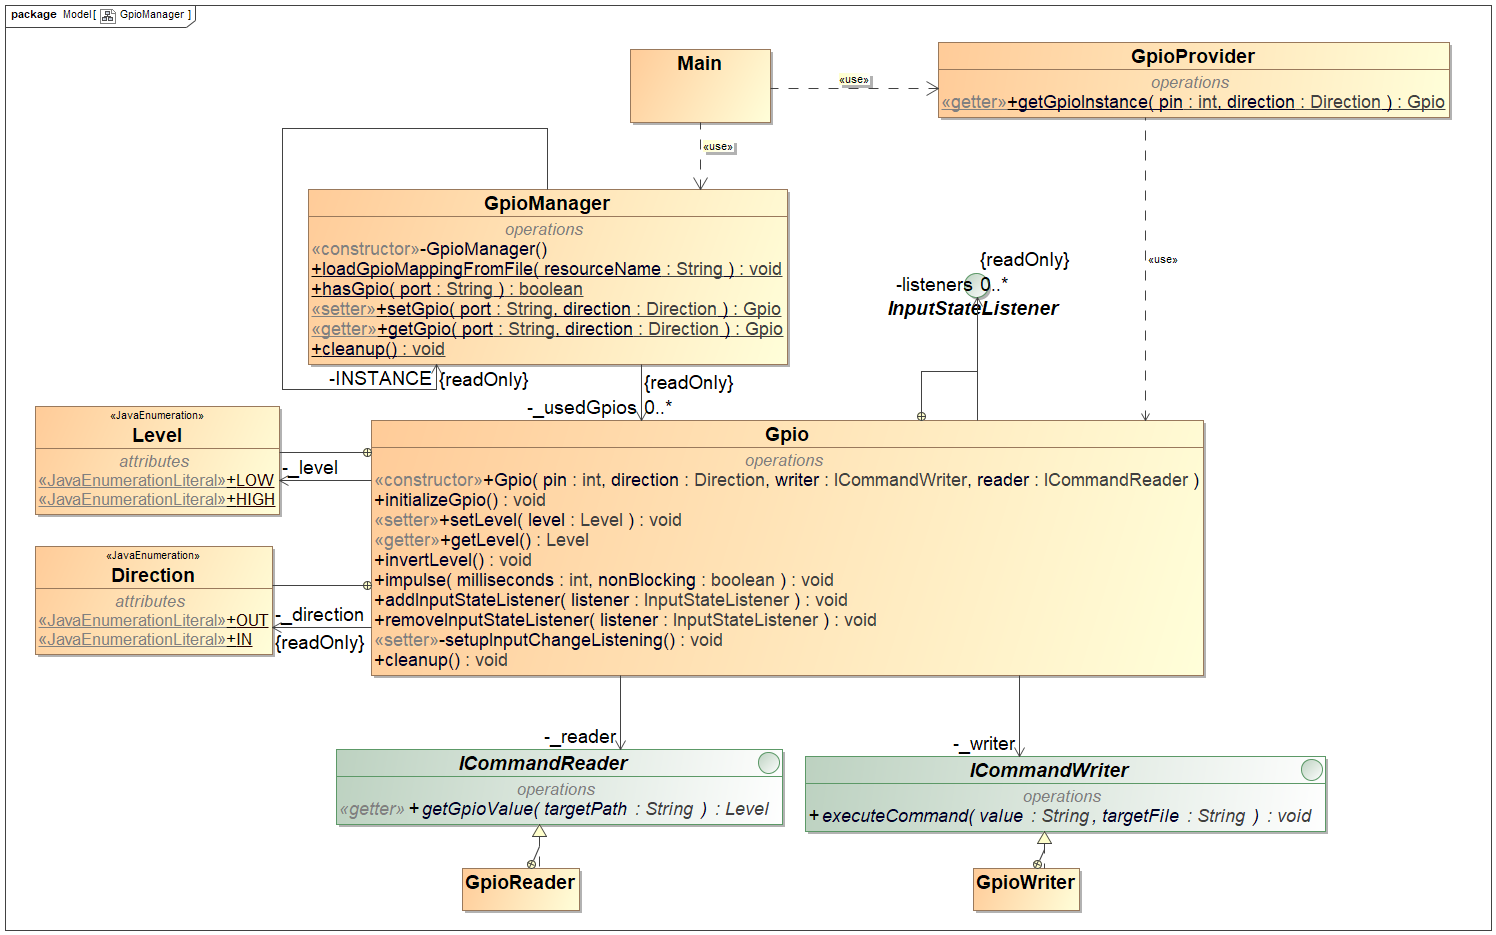
\includegraphics[width=150mm, keepaspectratio]{figures/impl/GpioManager.png}
	\caption{Gpio manager class diagram}
	\label{fig:gpiomanagerClass}
\end{figure}
On \autoref{fig:gpiomanagerClass}, a class diagram shows the re-factored structure of the component. This structure gives an advantage that the file operation dependencies are extracted into interfaces, which we can be easily mocked. The following code snippet shows how a fake object can be created and verified. 

\begin{lstlisting}[language = Java]
private static final String GPIOFOLDER = "/sys/class/gpio/";
// Create a fake class which behaves as any ICommandWriter class
@Mock
private ICommandWriter writer = Mockito.mock(ICommandWriter.class);
// Verify that the 'writer' fake object have been called 
// with 1 time during the execution with these exact parameters
Mockito.verify(writer, Mockito.times(1)).executeCommand(String.valueOf(67), GPIOFOLDER + "export");
\end{lstlisting}

As explained before the static methods can only be mocked with PowerMock, thus the following example shows how to make the GpioProvider to return a fake Gpio instance when the \textit{getGpioInstance} method is called with parameters: 86, Gpio.Direction.IN. Therefore in any further tests we can examine the mGpio instance as explained before.

\begin{lstlisting}
@RunWith(PowerMockRunner.class)
@PrepareForTest(GpioProvider.class)
public class GpioManagerTest{
	@Mock
	private Gpio mGpio = Mockito.mock(Gpio.class);
	
	@Before
	public void initEnv(){
		// Setup powermockito for static GpioProvider mocking
		PowerMockito.mockStatic(GpioProvider.class);
		// For these specific parameters, return the mGpio parameter
		PowerMockito.when(GpioProvider.getGpioInstance(86, Gpio.Direction.IN)).thenReturn(mGpio);
	}
}
\end{lstlisting}

Naturally a unit test should cover only one class, consequently if we consider the previously described structure (shown in \autoref{fig:gpiomanagerClass}), 6 unit test classes should be created (note that Level and Direction objects are only enumerables). Although there is no need to test basic file operation functions, provided by the Java framework in the GpioWriter and GpioReader classes and in addition there is no advantage to test the Main and GpioProvider classes, because there is no such a complex logic which should be verified by a test.

\paragraph{FS-2: Occupancy detection} The occupancy information handling components are the Section Occupancy Query (in C++ language) and the Occupancy Query elements (written in Xtend). The information flow between these components is based on S88 serial port connection. In this case this test implementation requires an S88 connection to the Arduino hardware element, because there is no virtual serial port simulators for Windows available on the market. Otherwise the C++ component can be separately verified that, it is collecting all the informations from the sections with Google Test. The Occupancy Query component runs on Java Virtual Machine, so JUnit 5 can be used without a problem. 

\begin{figure}[ht]
	\centering
	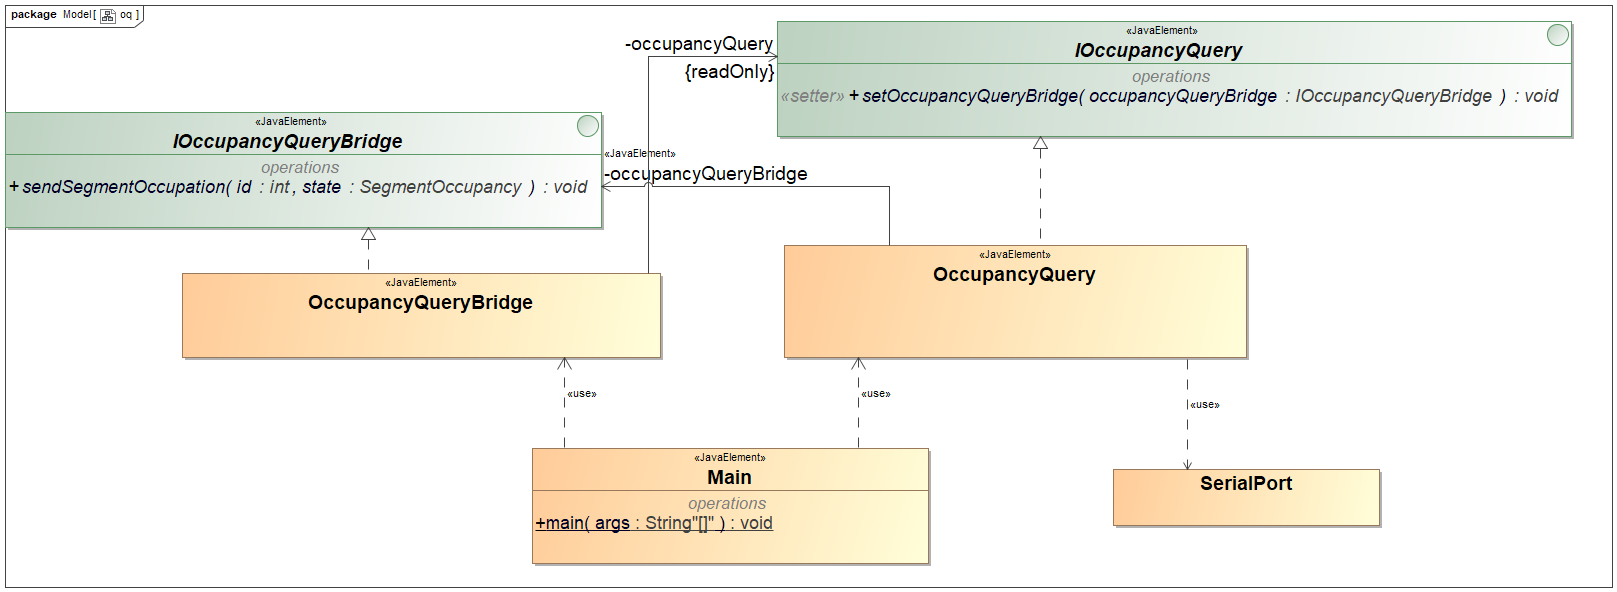
\includegraphics[width=150mm, keepaspectratio]{figures/impl/oq.png}
	\caption{Occupancy Query class diagram}
	\label{fig:occupancyqueryClass}
\end{figure}
The class structure of the Occupancy Query component is shown in \autoref{fig:occupancyqueryClass}, which describes the separation of a OccupancyQueryBridge, OccupancyQuery and Main class with their interfaces. The advantage of this architecture is the Occupancy calculation logic is well-separated from the message handling (in the OccupancyQueryBridge) logic. The obstacle to implement hardware independent test cases is the serial port dependency in the OccupancyQuery, for which the component must be re-factored. In addition the OccupancyQuery have dependencies to the SegmentOccupancy message type and for message handling elements, which should be also faked during the test executions.

\paragraph{FS-3: Track element controller} The next component have additional dependencies to the Turnout and SegmentState messages, to be able to perceive any state change on the track. In order to supervise the sections, the Track element controller must rely on the messaging service component aligned with the track configuration properties. The currently applicable version from the PowerMock is still in beta state, but until this point it was working properly. Unfortunately I have faced an issue, when I tried to mock a static method with a parameter of a static instance. The PowerMock already assigned the issue, but there is no bugfix implementation yet for the problem. Apart from that the architecture can also be reviewed to avoid static classes where it is not necessary.

\paragraph{FS-4: Safety Logic} The component level implementation of the Safety Logic consists of high level model based validators, from which a Java code was generated. In addition there is no need to test the glue code for these generated models. The system level Safety Logic also relies on generated Java code from the EMF model, nevertheless the decision-making logic is written in Xtend. This implementation also follows the previously described application and communication bridge architecture, but have a purely separated track refreshing algorithm. There are several shutdown strategies, which can be tested with this algorithm together. In addition this component also have dependencies to the SendAllStatus, SegmentOccupancy, TurnoutState, SegmentState and ComputerVisionObjectPositions messages with the communication services also.

\paragraph{FS-5: DashBoard} This feature set and component is responsible for controlling and visualizing the status of the track elements. Therefore it is handling mainly message communication and there is no safety-critical responsibility.

\subsection{Integration tests}
Through the messaging service every component can be controlled and observed, therefore in an integration test cases sending a specific message to the topic (to which the observed component is subscribed) can give an input to the observed component. For example to create an input for the Barrier component (which moves a physical barrier up or down on the track, if the supervised sections are occupied), a SegmentOccupancyChanged message must be sent to the topic of the supervised sections (15th or 24th). The component must implement ISegmentOccupancyChangedListener interface to get notification about a segment occupancy change event and handle every action. The following code shows the interface for a segment occupancy change and and example for subscribing mechanism.

\begin{lstlisting}[language = Java]
enum SegmentOccupancy {
	FREE,
	OCCUPIED
}

interface ISegmentOccupancyChangeListener {
	def void onSegmentOccupancyChange(int id, SegmentOccupancy oldValue, SegmentOccupancy newValue)
}

@Data
class SegmentOccupancyMessage extends InternalMessage {
	int segmentId
	SegmentOccupancy state
}

// subscribing to the 15th and 24th segment topics
val supervisedSections = #{15, 24}
val occupancyTopics = TopicFactory::createSegmentTopics(supervisedSections, #{SegmentOccupancyMessage}).toSet
\end{lstlisting}

A messaging dispatcher component, called TrackCommunicationServiceLocator provides an opportunity to send a specific message to the predefined topic which can be used by any component with the inheritance of AbstractCommunicationComponent abstract class. For example it is possible to send a SegmentOccupancy message to the subscribers through the trackElementCommander field, which is shown in the next code snippet.

\begin{lstlisting}[language = Java]
abstract class AbstractCommunicationComponent implements Runnable {
	protected val TrackCommunicationServiceLocator locator
}

class TrackCommunicationServiceLocator {
	@Accessors(PUBLIC_GETTER, PRIVATE_SETTER) val ITrackElementStateSender trackElementStateSender
	@Accessors(PUBLIC_GETTER, PRIVATE_SETTER) val ITrackElementCommander trackElementCommander
	@Accessors(PUBLIC_GETTER, PRIVATE_SETTER) val ITrainCommander trainCommander
	@Accessors(PUBLIC_GETTER, PRIVATE_SETTER) val IDccCommander dccCommander
	
	@Accessors(PUBLIC_GETTER, PRIVATE_SETTER) val ITrackElementCommandCallback trackElementCommandCallback
	@Accessors(PUBLIC_GETTER, PRIVATE_SETTER) val ITrackElementStateRegistry trackElementStateRegistry
	@Accessors(PUBLIC_GETTER, PRIVATE_SETTER) val ITrainSpeedStateRegistry trainSpeedStateRegistry
	@Accessors(PUBLIC_GETTER, PRIVATE_SETTER) val ISendAllStatusCommandCallback sendAllStatusCallback
	@Accessors(PUBLIC_GETTER, PRIVATE_SETTER) val IComputerVisionCallback computerVisionCallback
}

class TrackElementCommander implements ITrackElementCommander {
	var protected MessagingService mms
	
	/**
	* Send a command to a segment, denoted by its ID.
	*/
	override sendSegmentCommand(int id, SegmentState state) {
		mms.sendMessage(new SegmentCommand(id, state))
	}
}

class SampleOccupancySender extends AbstractCommunicationComponent {
	override sendSegmentOccupation(int id, SegmentOccupancy state) {
		locator.trackElementStateSender.sendSegmentOccupation(id, state)
	}
}
\end{lstlisting}

\subsection{System tests}
In order to execute system tests the demonstrator table must be started properly with the safety logic also. To start when the table is switched on, the BBB, PI and Arduino hardware elements are configured to start automatically with the basic services. These are the SectionOccupancyQuery, OccupancyQuery, TrackElementController and Dashboard components. The Safety Logic implementations prerequisites are to have these services already running on the network. Therefore after every automatically starting service is up, the component level safety logic service can be started on every BBB.

\section{Test Results}
\begin{figure}[ht]
	\centering
	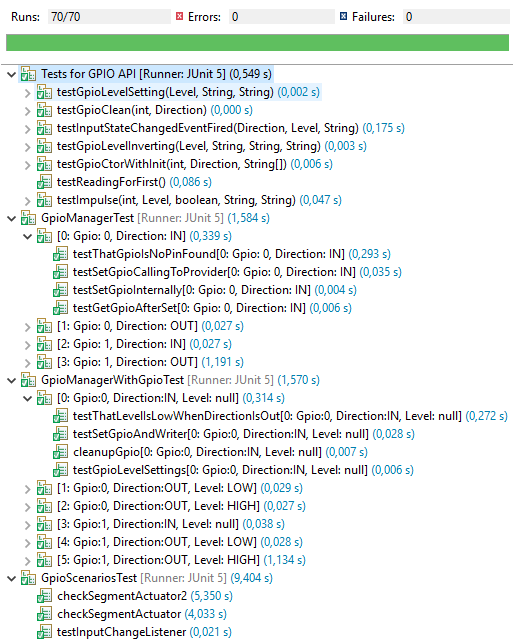
\includegraphics[width=100mm, keepaspectratio]{figures/impl/gpioTests.png}
	\caption{Implemented test cases for GPIO Manager component}
	\label{fig:gpiomanagerTests}
\end{figure}
\paragraph{Unit test results} Thus I have implemented unit test classes for Gpio and GpioManager separately (shown as "Tests for GPIO API" and "GpioManagerTest" groups on \autoref{fig:gpiomanagerTests}), then test cases for verifying the GpioManager with Gpio together. The GpioScenariosTest is stands for running an initialization test with all the components together in the final environment (in Debian operating system on the BBB). All the previous test classes are parameterized with more than one GPIO pin and all (in and out) directions.

\begin{figure}[ht]
	\centering
	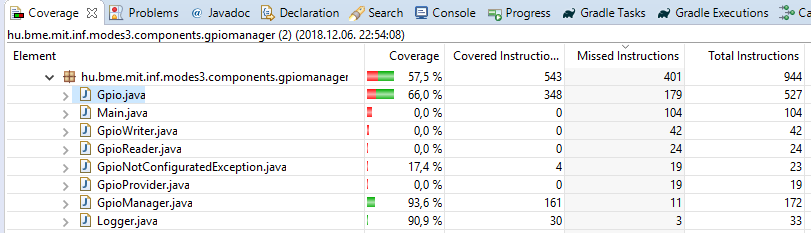
\includegraphics[width=150mm, keepaspectratio]{figures/impl/gpioCoverage.png}
	\caption{Code coverage measurement for GPIO Manager component}
	\label{fig:gpiomanagerCoverage}
\end{figure}
For each component the requirement was to achieve an 80\% code coverage. It is unnecessary to test classes without any business logic, so the Main, GpioWriter, GpioReader, GpioNotConfiguredException, GpioProvider and Logger classes have been skipped. The GpioManager code coverage is 93.6\% which is acceptable, but for the Gpio class it is 66.0\% which is below the required percentage. The root cause for the low rate is that there are hardly reachable error handling branches in the algorithm, which is not covered by any test.

\paragraph{System test results} The first attempt was failed, because of the wrong initialization of 2 segments. An issue is assigned with the title of: "Failed initialization during startup for section 8, 15".
\begin{table}[ht]
	\caption{System test result for procedure FSS-1 (1)}
	\label{table:SystemTestProcedure-1-Result1}
	\begin{center}
		\renewcommand{\arraystretch}{1.8}
		\begin{tabu} 
			to 0.9 \textwidth
			{  X[1.5, c] X[1.5, c] X[c]  }
			\toprule
			Test case name           & Actual results                                                                & Test result \\ \midrule
			1-1: change all turnout  & It was traceable with the DashBoard functionalities                           & Passed      \\
			1-2: disable all segment & S8 and S5 segments were remained disabled in the initialization phase already & Failed      \\
			1-3: enable all segment  & S8 and S5 segments were remained disabled in the initialization phase already & Failed      \\ \bottomrule
		\end{tabu}
	\end{center}
\end{table}

The second attempt was successful without any issue, therefore changing all turnout states from the dashboard was successful as well as segment availability change. In case of a disabled segment, a train have stopped on that exact segment, verifying that the change was effective and there was no power supply on the segment.
 
\begin{table}[ht]
	\caption{System test result for test procedure FSS-1 (2)}
	\label{table:SystemTestProcedure-1-Result2}
	\begin{center}
		\renewcommand{\arraystretch}{1.8}
		\begin{tabu} 
			to 0.9 \textwidth
			{  X[1.5, c] X[1.5, c] X[c] }
			\toprule
			Test case name           & Actual results                                      & Test result \\ \midrule
			1-1: change all turnout  & It was traceable with the DashBoard functionalities & Passed      \\
			1-2: disable all segment & All segment status were changed to disabled         & Passed      \\
			1-3: enable all segment  & All segment status were changed to enabled          & Passed      \\ \bottomrule
		\end{tabu}
	\end{center}
\end{table}

\begin{table}[H]
	\caption{System test result for test procedure FSS-2}
	\label{table:SystemTestProcedure-2-Result}
	\begin{center}
		\renewcommand{\arraystretch}{1.8}
		\begin{tabu} 
			to 0.9 \textwidth
			{  X[1.5, c] X[1.5, c] X[c] }
			\toprule
			Test case name       & Actual results       & Test result \\ \midrule
			2-1: turnout derail  & Segment was disabled & Passed      \\
			2-2: train collision & Segment was disabled & Passed      \\ \bottomrule
		\end{tabu}
	\end{center}
\end{table}

\section{Incident report}
One problem was found during the system test, which is assigned by the following \autoref{table:incident-1}
\begin{table}[H]
	\caption{System test result for procedure FSS-1}
	\label{table:incident-1}
	\begin{center}
		\renewcommand{\arraystretch}{1.8}
		\begin{tabu} 
			to 0.9 \textwidth
			{ X[c] X[c] X[c] X[c] }
			\toprule
			Issue title                                            & Severity & How to reproduce                                                                                & Description                                                                                                                      \\ \midrule
			Failed initialization during startup for section 8, 15 & Low      & The first startup of the demonstrator table ends in a state of 2 failed section initialization. & A possible workaround is to restart the whole table in less then a few minute. Because in this case it is initialized correctly. \\ \bottomrule
		\end{tabu}
	\end{center}
\end{table}


%----------------------------------------------------------------------------
\chapter{Summary}\label{chapter:Summary}
%----------------------------------------------------------------------------
During my thesis work, I got to know a test documentation standard \cite{IEEE13}. This approach was used to design a maintainable and detailed test plan for the MoDeS$^3$ project. The demonstrator system is a multi-layered application with off-the-shelf and custom hardware elements. Additionally for these microcontrollers, custom software components were developed to satisfy the required environment to control the track elements. Therefore I have detailed all the necessary software and hardware units to create a systematic test plan for the demonstrator system, which is mainly relies on the architecture and can be easily maintainable by the developers. The previously defined test cases was implemented in a safety-critical aspect also in unit, integration and system level.

I have found and detailed several improvable point in the \autoref{TestImpl:MODES}, which can take place in the future. These are especially component related implementation improvements, which can help testability in the following development phases.
%% !TeX spellcheck = hu_HU
% !TeX encoding = UTF-8
% !TeX program = xelatex
%----------------------------------------------------------------------------
\chapter{A \LaTeX-sablon használata}
%----------------------------------------------------------------------------

Ebben a fejezetben röviden, implicit módon bemutatjuk a sablon használatának módját, ami azt jelenti, hogy sablon használata ennek a dokumentumnak a forráskódját tanulmányozva válik teljesen világossá. Amennyiben a szoftver-keretrendszer telepítve van, a sablon alkalmazása és a dolgozat szerkesztése \LaTeX-ben a sablon segítségével tapasztalataink szerint jóval hatékonyabb, mint egy WYSWYG (\emph{What You See is What You Get}) típusú szövegszerkesztő esetén (pl. Microsoft Word, OpenOffice).

%----------------------------------------------------------------------------
\section{Címkék és hivatkozások}
%----------------------------------------------------------------------------
A \LaTeX~dokumentumban címkéket (\verb+\label+) rendelhetünk ábrákhoz, táblázatokhoz, fejezetekhez, listákhoz, képletekhez stb. Ezekre a dokumentum bármely részében hivatkozhatunk, a hivatkozások automatikusan feloldásra kerülnek.

A sablonban makrókat definiáltunk a hivatkozások megkönnyítéséhez. Ennek megfelelően minden ábra (\emph{figure}) címkéje \verb+fig:+ kulcsszóval kezdődik, míg minden táblázat (\emph{table}), képlet (\emph{equation}), fejezet (\emph{section}) és lista (\emph{listing}) rendre a \verb+tab:+, \verb+eq:+, \verb+sec:+ és \verb+lst:+ kulcsszóval kezdődik, és a kulcsszavak után tetszőlegesen választott címke használható. Ha ezt a konvenciót betartjuk, akkor az előbbi objektumok számára rendre a \verb+\figref+, \verb+\tabref+, \verb+\eqref+, \verb+\sectref+ és \verb+\listref+ makrókkal hivatkozhatunk. A makrók paramétere a címke, amelyre hivatkozunk (a kulcsszó nélkül). Az összes említett hivatkozástípus, beleértve az \verb+\url+ kulcsszóval bevezetett web-hivatkozásokat is a  \verb+hyperref+\footnote{Segítségével a dokumentumban megjelenő hivatkozások nem csak dinamikussá válnak, de színezhetők is, bővebbet erről a csomag dokumentációjában találunk. Ez egyúttal egy példa lábjegyzet írására.} csomagnak köszönhetően aktívak a legtöbb PDF-nézegetőben, rájuk kattintva a dokumentum megfelelő oldalára ugrik a PDF-néző vagy a megfelelő linket megnyitja az alapértelmezett böngészővel. A \verb+hyperref+ csomag a kimeneti PDF-dokumentumba könyvjelzőket is készít a tartalomjegyzékből. Ez egy szintén aktív tartalomjegyzék, amelynek elemeire kattintva a nézegető behozza a kiválasztott fejezetet.

%----------------------------------------------------------------------------
\section{Ábrák és táblázatok}
%----------------------------------------------------------------------------
Használjunk vektorgrafikus ábrákat, ha van rá módunk. PDFLaTeX használata esetén PDF formátumú ábrákat lehet beilleszteni könnyen, az EPS (PostScript) vektorgrafikus képformátum beillesztését a PDFLaTeX közvetlenül nem támogatja (de lehet konvertálni, lásd később). Ha vektorgrafikus formában nem áll rendelkezésünkre az ábra, akkor a  veszteségmentes PNG, valamint a veszteséges JPEG formátumban érdemes elmenteni.  Figyeljünk arra, hogy ilyenkor a képek felbontása elég nagy legyen ahhoz, hogy nyomtatásban is megfelelő minőséget nyújtson (legalább 300 dpi javasolt). A dokumentumban felhasznált képfájlokat a dokumentum forrása mellett érdemes tartani, archiválni, mivel ezek hiányában a dokumentum nem fordul újra. Ha lehet, a vektorgrafikus képeket vektorgrafikus formátumban is érdemes elmenteni az újrafelhasználhatóság (az átszerkeszthetőség) érdekében.

Kapcsolási rajzok legtöbbször kimásolhatók egy vektorgrafikus programba (pl. CorelDraw) és onnan nagyobb felbontással raszterizálva kimenthatők PNG formátumban. Ugyanakkor kiváló ábrák készíthetők Microsoft Visio vagy hasonló program használatával is: Visio-ból az ábrák közvetlenül PDF-be is menthetők.

Lehetőségeink Matlab ábrák esetén:
\begin{itemize}
	\item Képernyőlopás (\emph{screenshot}) is elfogadható minőségű lehet a dokumentumban, de általában jobb felbontást is el lehet érni más módszerrel.
	\item A Matlab ábrát a \verb+File/Save As+ opcióval lementhetjük PNG formátumban (ugyanaz itt is érvényes, mint korábban, ezért nem javasoljuk).
	\item A Matlab ábrát az \verb+Edit/Copy figure+ opcióval kimásolhatjuk egy vektorgrafikus programba is és onnan nagyobb felbontással raszterizálva kimenthatjük PNG formátumban (nem javasolt).
	\item Javasolt megoldás: az ábrát a \verb+File/Save As+ opcióval EPS \emph{vektorgrafikus} formátumban elmentjük, PDF-be konvertálva beillesztjük a dolgozatba.
\end{itemize}
Az EPS kép az \verb+epstopdf+ programmal\footnote{a korábban említett \LaTeX-disztribúciókban megtalálható} konvertálható PDF formátumba. Célszerű egy batch-fájlt készíteni az összes EPS ábra lefordítására az alábbi módon (ez Windows alatt működik).
\begin{lstlisting}
@echo off
for %%j in (*.eps) do (
echo converting file "%%j"
epstopdf "%%j"
)
echo done .
\end{lstlisting}

Egy ilyen parancsfájlt (\verb+convert.cmd+) elhelyeztük a sablon \verb+figures\eps+ könyvtárába, így a felhasználónak csak annyi a dolga, hogy a \verb+figures\eps+ könyvtárba kimenti az EPS formátumú vektorgrafikus képet, majd lefuttatja a \verb+convert.cmd+ parancsfájlt, ami PDF-be konvertálja az EPS fájlt.

Ezek után a PDF-ábrát ugyanúgy lehet a dokumentumba beilleszteni, mint a PNG-t vagy a JPEG-et. A megoldás előnye, hogy a lefordított dokumentumban is vektorgrafikusan tárolódik az ábra, így a mérete jóval kisebb, mintha raszterizáltuk volna beillesztés előtt. Ez a módszer minden -- az EPS formátumot ismerő -- vektorgrafikus program (pl. CorelDraw) esetén is használható.

A képek beillesztésére \az+\refstruc{sec:LatexTools}ben mutattunk be példát (\refstruc{fig:TeXstudio}). Az előző mondatban egyúttal az automatikusan feloldódó ábrahivatkozásra is láthatunk példát. Több képfájlt is beilleszthetünk egyetlen ábrába. Az egyes képek közötti horizontális és vertikális margót metrikusan szabályozhatjuk (\refstruc{fig:HVSpaces}). Az ábrák elhelyezését számtalan tipográfiai szabály egyidejű teljesítésével a fordító maga végzi, a dokumentum írója csak preferenciáit jelezheti a fordító felé (olykor ez bosszúságot is okozhat, ilyenkor pl. a kép méretével lehet játszani).

\begin{figure}[!ht]
	\centering
	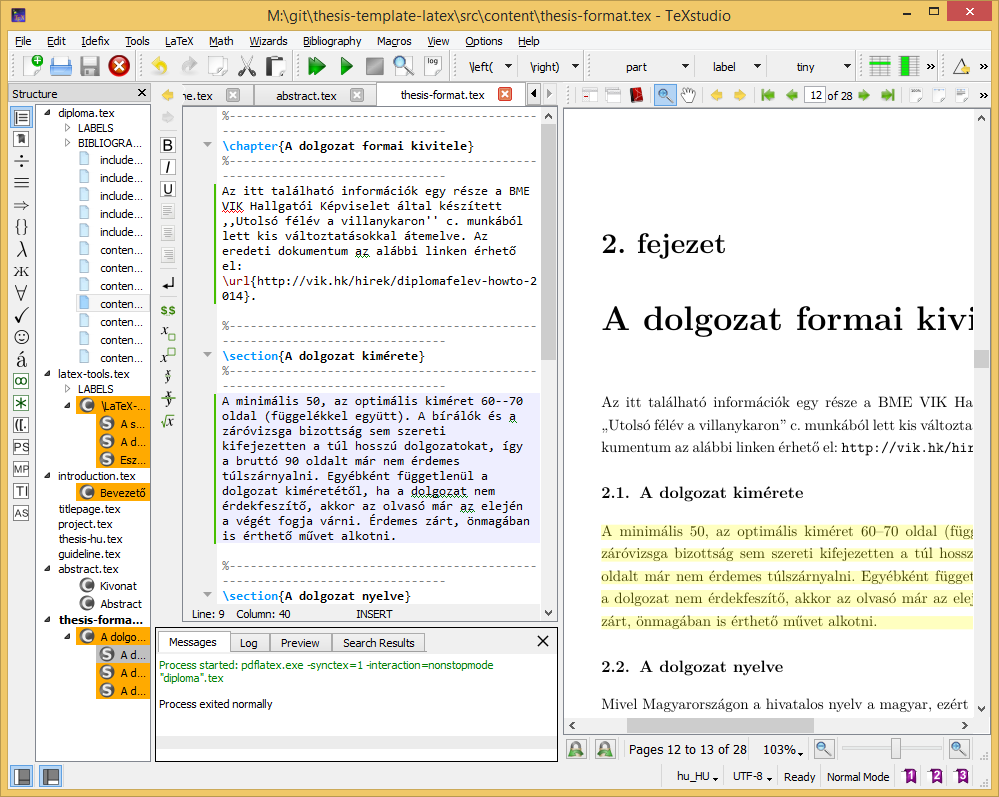
\includegraphics[width=67mm, keepaspectratio]{figures/TeXstudio.png}\hspace{1cm}
	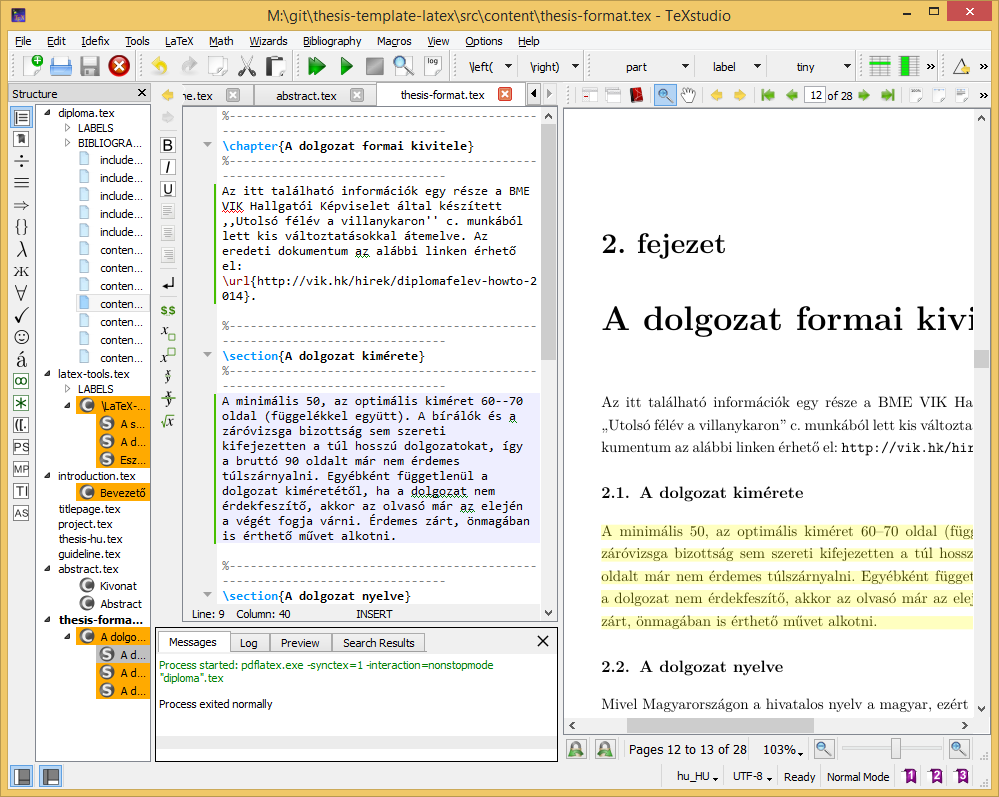
\includegraphics[width=67mm, keepaspectratio]{figures/TeXstudio.png}\\\vspace{5mm}
	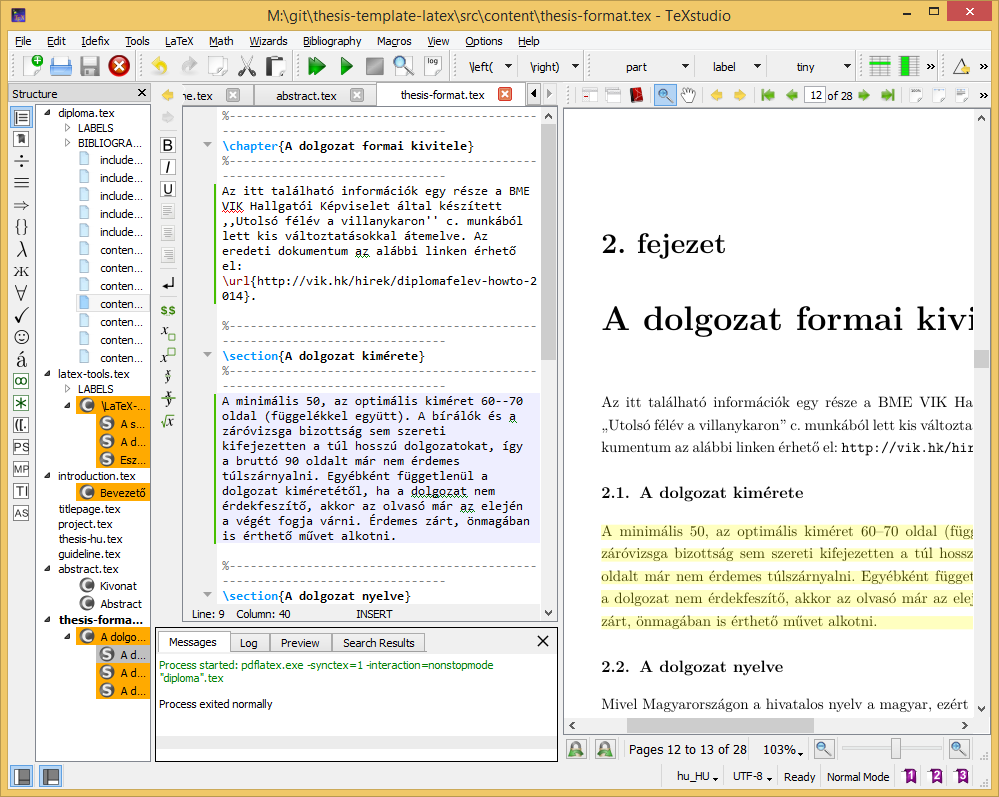
\includegraphics[width=67mm, keepaspectratio]{figures/TeXstudio.png}\hspace{1cm}
	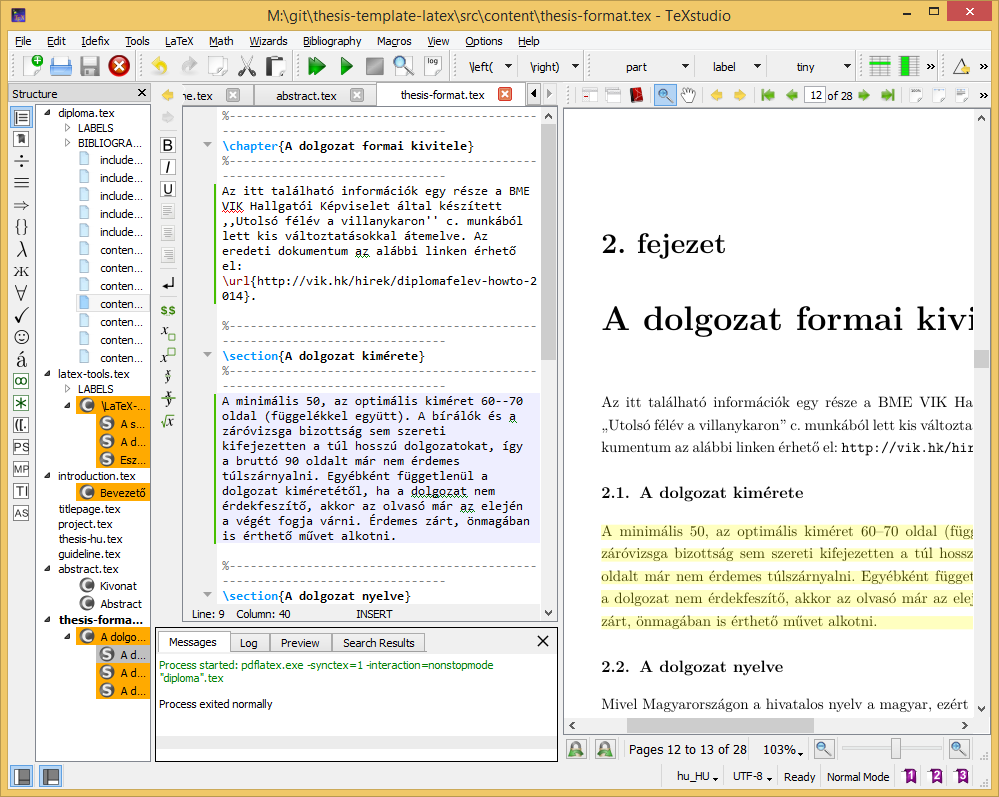
\includegraphics[width=67mm, keepaspectratio]{figures/TeXstudio.png}
	\caption{Több képfájl beillesztése esetén térközöket is érdemes használni.}
	\label{fig:HVSpaces}
\end{figure}

A táblázatok használatára \aref{tab:TabularExample}~táblázat mutat példát. A táblázatok formázásához hasznos tanácsokat találunk a \verb+booktabs+ csomag dokumentációjában.

\begin{table}[ht]
	\footnotesize
	\centering
	\begin{tabular}{ l c c }
		\toprule
		Órajel & Frekvencia & Cél pin \\
		\midrule
		CLKA & 100 MHz & FPGA CLK0\\
		CLKB & 48 MHz  & FPGA CLK1\\
		CLKC & 20 MHz  & Processzor\\
		CLKD & 25 MHz  & Ethernet chip \\
		CLKE & 72 MHz  & FPGA CLK2\\
		XBUF & 20 MHz  & FPGA CLK3\\
		\bottomrule
	\end{tabular}
	\caption{Az órajel-generátor chip órajel-kimenetei.}
	\label{tab:TabularExample}
\end{table}


%----------------------------------------------------------------------------
\section{Felsorolások és listák}
%----------------------------------------------------------------------------
Számozatlan felsorolásra mutat példát a jelenlegi bekezdés:
\begin{itemize}
	\item \emph{első bajusz:} ide lehetne írni az első elem kifejését,
	\item \emph{második bajusz:} ide lehetne írni a második elem kifejését,
	\item \emph{ez meg egy szakáll:} ide lehetne írni a harmadik elem kifejését.
\end{itemize}

Számozott felsorolást is készíthetünk az alábbi módon:
\begin{enumerate}
	\item \emph{első bajusz:} ide lehetne írni az első elem kifejését, és ez a kifejtés így néz ki, ha több sorosra sikeredik,
	\item \emph{második bajusz:} ide lehetne írni a második elem kifejését,
	\item \emph{ez meg egy szakáll:} ide lehetne írni a harmadik elem kifejését.
\end{enumerate}
A felsorolásokban sorok végén vessző, az utolsó sor végén pedig pont a szokásos írásjel. Ez alól kivételt képezhet, ha az egyes elemek több teljes mondatot tartalmaznak.

Listákban a dolgozat szövegétől elkülönítendő kódrészleteket, programsorokat, pszeudo-kódokat jeleníthetünk meg (\ref{lst:Example}.~kódrészlet).
\begin{lstlisting}[caption=A fenti számozott felsorolás \LaTeX-forráskódja,label=lst:Example]
\begin{enumerate}
	\item \emph{els(*@ő@*) bajusz:} ide lehetne írni az els(*@ő@*) elem kifejését,
	és ez a kifejtés így néz ki, ha több sorosra sikeredik,
	\item \emph{második bajusz:} ide lehetne írni a második elem kifejését,
	\item \emph{ez meg egy szakáll:} ide lehetne írni a harmadik elem kifejését.
\end{enumerate}
\end{lstlisting}
A lista keretét, háttérszínét, egész stílusát megválaszthatjuk. Ráadásul különféle programnyelveket és a nyelveken belül kulcsszavakat is definiálhatunk, ha szükséges. Erről bővebbet a \verb+listings+ csomag hivatalos leírásában találhatunk.

%----------------------------------------------------------------------------
\section{Képletek}
%----------------------------------------------------------------------------
Ha egy formula nem túlságosan hosszú, és nem akarjuk hivatkozni a szövegből, mint például a $e^{i\pi}+1=0$ képlet, \emph{szövegközi képletként} szokás leírni. Csak, hogy másik példát is lássunk, az $U_i=-d\Phi/dt$ Faraday-törvény a $\rot E=-\frac{dB}{dt}$ differenciális alakban adott Maxwell-egyenlet felületre vett integráljából vezethető le. Látható, hogy a \LaTeX-fordító a sorközöket betartja, így a szöveg szedése esztétikus marad szövegközi képletek használata esetén is.

Képletek esetén az általános konvenció, hogy a kisbetűk skalárt, a kis félkövér betűk ($\mathbf{v}$) oszlopvektort -- és ennek megfelelően $\mathbf{v}^T$ sorvektort -- a kapitális félkövér betűk ($\mathbf{V}$) mátrixot jelölnek. Ha ettől el szeretnénk térni, akkor az alkalmazni kívánt jelölésmódot célszerű külön alfejezetben definiálni. Ennek megfelelően, amennyiben $\mathbf{y}$ jelöli a mérések vektorát, $\mathbf{\vartheta}$ a paraméterek vektorát és $\hat{\mathbf{y}}=\mathbf{X}\vartheta$ a paraméterekben lineáris modellt, akkor a \emph{Least-Squares} értelemben optimális paraméterbecslő $\hat{\mathbf{\vartheta}}_{LS}=(\mathbf{X}^T\mathbf{X})^{-1}\mathbf{X}^T\mathbf{y}$ lesz.

Emellett kiemelt, sorszámozott képleteket is megadhatunk, ennél az \verb+equation+ és a \verb+eqnarray+ környezetek helyett a korszerűbb \verb+align+ környezet alkalmazását javasoljuk (több okból, különféle problémák elkerülése végett, amelyekre most nem térünk ki). Tehát
\begin{align}
\dot{\mathbf{x}}&=\mathbf{A}\mathbf{x}+\mathbf{B}\mathbf{u},\\
\mathbf{y}&=\mathbf{C}\mathbf{x},
\end{align}
ahol $\mathbf{x}$ az állapotvektor, $\mathbf{y}$ a mérések vektora és $\mathbf{A}$, $\mathbf{B}$ és $\mathbf{C}$ a rendszert leíró paramétermátrixok. Figyeljük meg, hogy a két egyenletben az egyenlőségjelek egymáshoz igazítva jelennek meg, mivel a mindkettőt az \& karakter előzi meg a kódban. Lehetőség van számozatlan kiemelt képlet használatára is, például
\begin{align}
\dot{\mathbf{x}}&=\mathbf{A}\mathbf{x}+\mathbf{B}\mathbf{u},\nonumber\\
\mathbf{y}&=\mathbf{C}\mathbf{x}\nonumber.
\end{align}
Mátrixok felírására az $\mathbf{A}\mathbf{x}=\mathbf{b}$ inhomogén lineáris egyenlet részletes kifejtésével mutatunk példát:
\begin{align}
\begin{bmatrix}
a_{11} & a_{12} & \dots & a_{1n}\\
a_{21} & a_{22} & \dots & a_{2n}\\
\vdots & \vdots & \ddots & \vdots\\
a_{m1} & a_{m2} & \dots & a_{mn}
\end{bmatrix}
\begin{pmatrix}x_1\\x_2\\\vdots\\x_n\end{pmatrix}=
\begin{pmatrix}b_1\\b_2\\\vdots\\b_m\end{pmatrix}.
\end{align}
A \verb+\frac+ utasítás hatékonyságát egy általános másodfokú tag átviteli függvényén keresztül mutatjuk be, azaz
\begin{align}
W(s)=\frac{A}{1+2T\xi s+s^2T^2}.
\end{align}
A matematikai mód minden szimbólumának és képességének a bemutatására természetesen itt nincs lehetőség, de gyors referenciaként hatékonyan használhatók a következő linkek:\\
\indent\url{http://www.artofproblemsolving.com/LaTeX/AoPS_L_GuideSym.php},\\
\indent\url{http://www.ctan.org/tex-archive/info/symbols/comprehensive/symbols-a4.pdf},\\
\indent\url{ftp://ftp.ams.org/pub/tex/doc/amsmath/short-math-guide.pdf}.\\
Ez pedig itt egy magyarázat, hogy miért érdemes \verb+align+ környezetet használni:\\
\indent\url{http://texblog.net/latex-archive/maths/eqnarray-align-environment/}.

%----------------------------------------------------------------------------
\section{Irodalmi hivatkozások}
\label{sec:HowtoReference}
%----------------------------------------------------------------------------
Egy \LaTeX~dokumentumban az irodalmi hivatkozások definíciójának két módja van. Az egyik a \verb+\thebibliograhy+ környezet használata a dokumentum végén, az \verb+\end{document}+ lezárás előtt.
\begin{lstlisting}
\begin{thebibliography}{9}

\bibitem{Lamport94} Leslie Lamport, \emph{\LaTeX: A Document Preparation System}.
Addison Wesley, Massachusetts, 2nd Edition, 1994.

\end{thebibliography}
\end{lstlisting}

Ezek után a dokumentumban a \verb+\cite{Lamport94}+ utasítással hivatkozhatunk a forrásra. A fenti megadás viszonylag kötetlen, a szerző maga formázza az irodalomjegyzéket (ami gyakran inkonzisztens eredményhez vezet).

Egy sokkal professzionálisabb módszer a BiB\TeX{} használata, ezért ez a sablon is ezt támogatja. Ebben az esetben egy külön szöveges adatbázisban definiáljuk a forrásmunkákat, és egy külön stílusfájl határozza meg az irodalomjegyzék kinézetét. Ez, összhangban azzal, hogy külön formátumkonvenció határozza meg a folyóirat-, a könyv-, a konferenciacikk- stb. hivatkozások kinézetét az irodalomjegyzékben (a sablon használata esetén ezzel nem is kell foglalkoznia a hallgatónak, de az eredményt célszerű ellenőrizni). felhasznált hivatkozások adatbázisa egy \verb+.bib+ kiterjesztésű szöveges fájl, amelynek szerkezetét a \Aref{lst:Bibtex} kódrészlet demonstrálja. A forrásmunkák bevitelekor a sor végi vesszők külön figyelmet igényelnek, mert hiányuk a BiB\TeX-fordító hibaüzenetét eredményezi. A forrásmunkákat típus szerinti kulcsszó vezeti be (\verb+@book+ könyv, \verb+@inproceedings+ konferenciakiadványban megjelent cikk, \verb+@article+ folyóiratban megjelent cikk, \verb+@techreport+ valamelyik egyetem gondozásában megjelent műszaki tanulmány, \verb+@manual+ műszaki dokumentáció esetén stb.). Nemcsak a megjelenés stílusa, de a kötelezően megadandó mezők is típusról-típusra változnak. Egy jól használható referencia a \url{http://en.wikipedia.org/wiki/BibTeX} oldalon található.

\begin{lstlisting}[caption=Példa szöveges irodalomjegyzék-adatbázisra Bib\TeX{} használata esetén.,label=lst:Bibtex]
@book{Wettl04,
  author    = {Ferenc Wettl and Gyula Mayer and Péter Szabó},
  publisher = {Panem Könyvkiadó},
  title     = {\LaTeX~kézikönyv},
  year      = {2004},
}

@article{Candy86,
  author       = {James C. Candy},
  journaltitle = {{IEEE} Trans.\ on Communications},
  month        = {01},
  note         = {\doi{10.1109/TCOM.1986.1096432}},
  number       = {1},
  pages        = {72--76},
  title        = {Decimation for Sigma Delta Modulation},
  volume       = {34},
  year         = {1986},
}

@inproceedings{Lee87,
  author    = {Wai L. Lee and Charles G. Sodini},
  booktitle = {Proc.\ of the IEEE International Symposium on Circuits and Systems},
  location  = {Philadelphia, PA, USA},
  month     = {05~4--7},
  pages     = {459--462},
  title     = {A Topology for Higher Order Interpolative Coders},
  vol       = {2},
  year      = {1987},
}

@thesis{KissPhD,
  author      = {Peter Kiss},
  institution = {Technical University of Timi\c{s}oara, Romania},
  month       = {04},
  title       = {Adaptive Digital Compensation of Analog Circuit Imperfections for Cascaded Delta-Sigma Analog-to-Digital Converters},
  type        = {phdthesis},
  year        = {2000},
}

@manual{Schreier00,
  author       = {Richard Schreier},
  month        = {01},
  note         = {\url{http://www.mathworks.com/matlabcentral/fileexchange/}},
  organization = {Oregon State University},
  title        = {The Delta-Sigma Toolbox v5.2},
  year         = {2000},
}

@misc{DipPortal,
  author       = {{Budapesti Műszaki és Gazdaságtudományi Egyetem Villamosmérnöki és Informatikai Kar}},
  howpublished = {\url{http://diplomaterv.vik.bme.hu/}},
  title        = {Diplomaterv portál (2011. február 26.)},
}

@incollection{Mkrtychev:1997,
  author    = {Mkrtychev, Alexey},
  booktitle = {Logical Foundations of Computer Science},
  doi       = {10.1007/3-540-63045-7_27},
  editor    = {Adian, Sergei and Nerode, Anil},
  isbn      = {978-3-540-63045-6},
  pages     = {266-275},
  publisher = {Springer Berlin Heidelberg},
  series    = {Lecture Notes in Computer Science},
  title     = {Models for the logic of proofs},
  url       = {http://dx.doi.org/10.1007/3-540-63045-7_27},
  volume    = {1234},
  year      = {1997},
}
\end{lstlisting}

A stílusfájl egy \verb+.sty+ kiterjesztésű fájl, de ezzel lényegében nem kell foglalkozni, mert vannak beépített stílusok, amelyek jól használhatók. Ez a sablon a BiB\TeX-et használja, a hozzá tartozó adatbázisfájl a \verb+mybib.bib+ fájl. Megfigyelhető, hogy az irodalomjegyzéket a dokumentum végére (a \verb+\end{document}+ utasítás elé) beillesztett \verb+\bibliography{mybib}+ utasítással hozhatjuk létre, a stílusát pedig ugyanitt a  \verb+\bibliographystyle{plain}+ utasítással adhatjuk meg. Ebben az esetben a \verb+plain+ előre definiált stílust használjuk (a sablonban is ezt állítottuk be). A \verb+plain+ stíluson kívül természetesen számtalan más előre definiált stílus is létezik. Mivel a \verb+.bib+ adatbázisban ezeket megadtuk, a BiB\TeX-fordító is meg tudja különböztetni a szerzőt a címtől és a kiadótól, és ez alapján automatikusan generálódik az irodalomjegyzék a stílusfájl által meghatározott stílusban.

Az egyes forrásmunkákra a szövegből továbbra is a \verb+\cite+ paranccsal tudunk hivatkozni, így \aref{lst:Bibtex}.~kódrészlet esetén a hivatkozások rendre \verb+\cite{Wettl04}+, \verb+\cite{Candy86}+, \verb+\cite{Lee87}+, \verb+\cite{KissPhD}+, \verb+\cite{Schreirer00}+,
\verb+\cite{Mkrtychev:1997}+ és \verb+\cite{DipPortal}+. Az egyes forrásmunkák sorszáma az irodalomjegyzék bővítésekor változhat. Amennyiben az aktuális számhoz illeszkedő névelőt szeretnénk használni, használjuk az \verb+\acite{}+ parancsot.

Az irodalomjegyzékben alapértelmezésben csak azok a forrásmunkák jelennek meg, amelyekre található hivatkozás a szövegben, és ez így alapvetően helyes is, hiszen olyan forrásmunkákat nem illik az irodalomjegyzékbe írni, amelyekre nincs hivatkozás.

Mivel a fordítási folyamat során több lépésben oldódnak fel a szimbólumok, ezért gyakran többször is le kell fordítani a dokumentumot. Ilyenkor ez első 1-2 fordítás esetleg szimbólum-feloldásra vonatkozó figyelmeztető üzenettel zárul. Ha hibaüzenettel zárul bármelyik fordítás, akkor nincs értelme megismételni, hanem a hibát kell megkeresni. A \verb+.bib+ fájl megváltoztatáskor sokszor nincs hatása a változtatásnak azonnal, mivel nem mindig fut újra a BibTeX fordító. Ezért célszerű a változtatás után azt manuálisan is lefuttatni (TeXstudio esetén \verb+Tools/Bibliography+).

Hogy a szövegbe ágyazott hivatkozások kinézetét demonstráljuk, itt most sorban meghivatkozzuk a \cite{Wettl04}, \cite{Candy86}, \cite{Lee87}, \cite{KissPhD}, \cite{Schreier00} és \acite{Mkrtychev:1997}\footnote{Informatikai témában gyakran hivatkozunk cikkeket a Springer LNCS valamely kötetéből, ez a hivatkozás erre mutat egy helyes példát.} forrásmunkát, valamint \acite{DipPortal} weboldalt.

Megjegyzendő, hogy az ékezetes magyar betűket is tartalmazó \verb+.bib+ fájl az \verb+inputenc+ csomaggal betöltött \verb+latin2+ betűkészlet miatt fordítható. Ugyanez a \verb+.bib+ fájl hibaüzenettel fordul egy olyan dokumentumban, ami nem tartalmazza a \verb+\usepackage[latin2]{inputenc}+ sort. Speciális igény esetén az irodalmi adatbázis általánosabb érvényűvé tehető, ha az ékezetes betűket speciális latex karakterekkel helyettesítjük a \verb+.bib+ fájlban, pl. á helyett \verb+\'{a}+-t vagy ő helyett \verb+\H{o}+-t írunk.

Oldaltörés következik (ld. forrás).
\newpage

%----------------------------------------------------------------------------
\section{A dolgozat szerkezete és a forrásfájlok}
%----------------------------------------------------------------------------
A diplomatervsablonban a TeX fájlok két alkönyvtárban helyezkednek el. Az \verb+include+ könyvtárban azok szerepelnek, amiket tipikusan nem kell szerkesztenünk, ezek a sablon részei (pl. címoldal). A \verb+content+ alkönyvtárban pedig a saját munkánkat helyezhetjük el. Itt érdemes az egyes fejezeteket külön \TeX{} állományokba rakni.

A diplomatervsablon (a kari irányelvek szerint) az alábbi fő fejezetekből áll:
\begin{enumerate}
	\item 1 oldalas \emph{tájékoztató} a szakdolgozat/diplomaterv szerkezetéről (\verb+include/guideline.tex+), ami a végső dolgozatból törlendő,
	\item \emph{feladatkiírás} (\verb+include/project.tex+), a dolgozat nyomtatott verzójában ennek a helyére kerül a tanszék által kiadott, a tanszékvezető által aláírt feladatkiírás, a dolgozat elektronikus verziójába pedig a feladatkiírás egyáltalán ne kerüljön bele, azt külön tölti fel a tanszék a diplomaterv-honlapra,
	\item \emph{címoldal} (\verb+include/titlepage.tex+),
	\item \emph{tartalomjegyzék} (\verb+thesis.tex+),
	\item a diplomatervező \emph{nyilatkozat}a az önálló munkáról (\verb+include/declaration.tex+),
	\item 1-2 oldalas tartalmi \emph{összefoglaló} magyarul és angolul, illetve elkészíthető még további nyelveken is (\verb+content/abstract.tex+),
	\item \emph{bevezetés}: a feladat értelmezése, a tervezés célja, a feladat indokoltsága, a diplomaterv felépítésének rövid összefoglalása (\verb+content/introduction.tex+),
	\item sorszámmal ellátott \emph{fejezetek}: a feladatkiírás pontosítása és részletes elemzése, előzmények (irodalomkutatás, hasonló alkotások), az ezekből levonható következtetések, a tervezés részletes leírása, a döntési lehetőségek értékelése és a választott megoldások indoklása, a megtervezett műszaki alkotás értékelése, kritikai elemzése, továbbfejlesztési lehetőségek,
	\item esetleges \emph{köszönetnyilvánítás}ok (\verb+content/acknowledgement.tex+),
	\item részletes és pontos \emph{irodalomjegyzék} (ez a sablon esetében automatikusan generálódik a \verb+thesis.tex+ fájlban elhelyezett \verb+\bibliography+ utasítás hatására, \az+\refstruc{sec:HowtoReference}ban leírtak szerint),
	\item \emph{függelékek} (\verb+content/appendices.tex+).
\end{enumerate}

A sablonban a fejezetek a \verb+thesis.tex+ fájlba vannak beillesztve \verb+\include+ utasítások segítségével. Lehetőség van arra, hogy csak az éppen szerkesztés alatt álló \verb+.tex+ fájlt fordítsuk le, ezzel lerövidítve a fordítási folyamatot. Ezt a lehetőséget az alábbi kódrészlet biztosítja a \verb+thesis.tex+ fájlban.
\begin{lstlisting}
\includeonly{
	guideline,%
	project,%
	titlepage,%
	declaration,%
	abstract,%
	introduction,%
	chapter1,%
	chapter2,%
	chapter3,%
	acknowledgement,%
	appendices,%
}
\end{lstlisting}

Ha az alábbi kódrészletben az egyes sorokat a \verb+%+ szimbólummal kikommentezzük, akkor a megfelelő \verb+.tex+ fájl nem fordul le. Az oldalszámok és a tartalomjegyék természetesen csak akkor billennek helyre, ha a teljes dokumentumot lefordítjuk.

%----------------------------------------------------------------------------
\newpage
\section{Alapadatok megadása}
%----------------------------------------------------------------------------
A diplomaterv alapadatait (cím, szerző, konzulens, konzulens titulusa) a \verb+thesis.tex+ fájlban lehet megadni.

%----------------------------------------------------------------------------
\section{Új fejezet írása}
%----------------------------------------------------------------------------
A főfejezetek külön \verb+content+ könyvtárban foglalnak helyet. A sablonhoz 3 fejezet készült. További főfejezeteket úgy hozhatunk létre, ha új \TeX~fájlt készítünk a fejezet számára, és a \verb+thesis.tex+ fájlban, a \verb+\include+ és \verb+\includeonly+ utasítások argumentumába felvesszük az új \verb+.tex+ fájl nevét.


%----------------------------------------------------------------------------
\section{Definíciók, tételek, példák}
%----------------------------------------------------------------------------

\begin{definition}[Fluxuskondenzátor térerőssége]
Lorem ipsum dolor sit amet, consectetur adipiscing elit, sed do eiusmod tempor incididunt ut labore et dolore magna aliqua. Ut enim ad minim veniam, quis nostrud exercitation ullamco laboris nisi ut aliquip ex ea commodo consequat.
\end{definition}

\begin{example}
Példa egy példára. Duis aute irure dolor in reprehenderit in voluptate velit esse cillum dolore eu fugiat nulla pariatur. Excepteur sint occaecat cupidatat non proident, sunt in culpa qui officia deserunt mollit anim id est laborum.
\end{example}

\begin{theorem}[Kovács tétele]
Duis aute irure dolor in reprehenderit in voluptate velit esse cillum dolore eu fugiat nulla pariatur. Excepteur sint occaecat cupidatat non proident, sunt in culpa qui officia deserunt mollit anim id est laborum.
\end{theorem}



% Acknowledgements
%~~~~~~~~~~~~~~~~~~~~~~~~~~~~~~~~~~~~~~~~~~~~~~~~~~~~~~~~~~~~~~~~~~~~~~~~~~~~~~~~~~~~~~
%%----------------------------------------------------------------------------
\chapter*{\koszonetnyilvanitas}\addcontentsline{toc}{chapter}{\koszonetnyilvanitas}
%----------------------------------------------------------------------------

Ez nem kötelező, akár törölhető is. Ha a szerző szükségét érzi, itt lehet köszönetet nyilvánítani azoknak, akik hozzájárultak munkájukkal ahhoz, hogy a hallgató a szakdolgozatban vagy diplomamunkában leírt feladatokat sikeresen elvégezze. A konzulensnek való köszönetnyilvánítás sem kötelező, a konzulensnek hivatalosan is dolga, hogy a hallgatót konzultálja.


% List of Figures, Tables
%~~~~~~~~~~~~~~~~~~~~~~~~~~~~~~~~~~~~~~~~~~~~~~~~~~~~~~~~~~~~~~~~~~~~~~~~~~~~~~~~~~~~~~
\listoffigures\addcontentsline{toc}{chapter}{\listfigurename}
\listoftables\addcontentsline{toc}{chapter}{\listtablename}


% Bibliography
%~~~~~~~~~~~~~~~~~~~~~~~~~~~~~~~~~~~~~~~~~~~~~~~~~~~~~~~~~~~~~~~~~~~~~~~~~~~~~~~~~~~~~~
%TODO what to do with nocite things
%\nocite{*}
\addcontentsline{toc}{chapter}{\bibname}
\bibliography{bib/mybib}



% Appendix
%~~~~~~~~~~~~~~~~~~~~~~~~~~~~~~~~~~~~~~~~~~~~~~~~~~~~~~~~~~~~~~~~~~~~~~~~~~~~~~~~~~~~~~
%----------------------------------------------------------------------------
\appendix
%----------------------------------------------------------------------------
\chapter*{\fuggelek}\addcontentsline{toc}{chapter}{\fuggelek}
\setcounter{chapter}{\appendixnumber}
%\setcounter{equation}{6} % a fofejezet-szamlalo az angol ABC 6. betuje (F) lesz
\numberwithin{equation}{section}
\numberwithin{figure}{section}
\numberwithin{lstlisting}{section}
%\numberwithin{tabular}{section}

%----------------------------------------------------------------------------
\section{Test cases for MoDeS$^3$ Unit Test Plan} \label{appendix:UnitTC}
%----------------------------------------------------------------------------

\subsection{GPIO manager}
\begin{table}[H]
	\caption{Test case 1-1}
	\label{table:TCase-FS1-1}
	\begin{center}
		\renewcommand{\arraystretch}{1.8}
		\begin{tabu} 
			to 0.9 \textwidth
			{  X[0.3, l] X[l] }
			\toprule
			Test case ID: 1-1 & Purpose: to test the GPIO initialization in input direction. \newline Priority: am \newline Tracing: FS-1/1.0 \\ \midrule
			Precondition      & The GPIO's necessary files are available.                                                                     \\
			Input             & Initialize the GPIO itself with input direction.                                                              \\
			Expected result   & The "both" string have been written to "edge" configuration file.                                             \\ \bottomrule
		\end{tabu}
	\end{center}
\end{table} 

\begin{table}[H]
	\caption{Test case 1-2}
	\label{table:TCase-FS1-2}
	\begin{center}
		\renewcommand{\arraystretch}{1.8}
		\begin{tabu} 
			to 0.9 \textwidth
			{  X[0.3, l] X[l] }
			\toprule
			Test case ID: 1-2 & Purpose: to test the GPIO pin input change listener while direction is input and the value is "0". \newline Priority: am \newline Tracing: FS-1/1.1 \\ \midrule
			Precondition      & The GPIO's necessary files are available.                                                                                                           \\
			Input             & The value file have been written to "0", considered as LOW.                                                                                         \\
			Expected result   & GPIO noticed the change and read the "value" configuration file content as LOW level.                                                               \\ \bottomrule
		\end{tabu}
	\end{center}
\end{table} 

\begin{table}[H]
	\caption{Test case 1-3}
	\label{table:TCase-FS1-3}
	\begin{center}
		\renewcommand{\arraystretch}{1.8}
		\begin{tabu} 
			to 0.9 \textwidth
			{  X[0.3, l] X[l] }
			\toprule
			Test case ID: 1-3 & Purpose: to test the GPIO pin change listener while direction is input and the value is "1". \newline Priority: am \newline Tracing: FS-1/1.2 \\ \midrule
			Precondition      & The GPIO's necessary files are available.                                                                                                     \\
			Input             & The value file have been written to "1" considered as HIGH.                                                                                   \\
			Expected result   & GPIO noticed the change and read the "value" configuration file content as HIGH level.                                                        \\ \bottomrule
		\end{tabu}
	\end{center}
\end{table} 

\begin{table}[H]
	\caption{Test case 1-4}
	\label{table:TCase-FS1-4}
	\begin{center}
		\renewcommand{\arraystretch}{1.8}
		\begin{tabu} 
			to 0.9 \textwidth
			{  X[0.3, l] X[l] }
			\toprule
			Test case ID: 1-4 & Purpose: to test the GPIO initialization in output direction. \newline Priority: am \newline Tracing: FS-1/2.0 \\ \midrule
			Precondition      & The GPIO's necessary files are available.                                                                      \\
			Input             & Initialize the GPIO itself with output direction.                                                              \\
			Expected result   & The "0" string have been written to "value" configuration file.                                                \\ \bottomrule
		\end{tabu}
	\end{center}
\end{table} 

\begin{table}[H]
	\caption{Test case 1-5}
	\label{table:TCase-FS1-5}
	\begin{center}
		\renewcommand{\arraystretch}{1.8}
		\begin{tabu} 
			to 0.9 \textwidth
			{  X[0.3, l] X[l] }
			\toprule
			Test case ID: 1-5 & Purpose: to test the GPIO pin's level setting to LOW. \newline Priority: am \newline Tracing: FS-1/2.1 \\ \midrule
			Precondition      & The GPIO's necessary files are available.                                                              \\
			Input             & Set the GPIO's level to LOW.                                                                           \\
			Expected result   & The "value" file has been modified with value "0"                                                      \\ \bottomrule
		\end{tabu}
	\end{center}
\end{table} 

\begin{table}[H]
	\caption{Test case 1-6}
	\label{table:TCase-FS1-6}
	\begin{center}
		\renewcommand{\arraystretch}{1.8}
		\begin{tabu} 
			to 0.9 \textwidth
			{  X[0.3, l] X[l] }
			\toprule
			Test case ID: 1-6 & Purpose: to test the GPIO pin's level setting to HIGH.  \newline Priority: am \newline Tracing: FS-1/2.2 \\ \midrule
			Precondition      & The GPIO's necessary files are available.                                                                \\
			Input             & Set the GPIO's level to HIGH.                                                                            \\
			Expected result   & The "value" file has been modified with value "1"                                                        \\ \bottomrule
		\end{tabu}
	\end{center}
\end{table} 

\subsection{Occupancy detection}

\begin{table}[H]
	\caption{Test case 2-1}
	\label{table:TCase-FS2-1}
	\begin{center}
		\renewcommand{\arraystretch}{1.8}
		\begin{tabu} 
			to 0.9 \textwidth
			{  X[0.3, l] X[l] }
			\toprule
			Test case ID: 2-1 & Purpose: to test the detection of segment occupancy (the train power consumption) through section occupancy query, when the specific segment is free\newline Priority: above middle \newline Tracing: (FS-2/1.0) \\ \midrule
			Precondition      & S88 serial port connection and available Arduino hardware element                                                                                                                                                \\
			Input             & Unclosed circuit between the specific segment's hardware elements elements                                                                                                                                       \\
			Expected result   & Occupancy components have queried free occupancy state                                                                                                                                                           \\ \bottomrule
		\end{tabu}
	\end{center}
\end{table} 

\begin{table}[H]
	\caption{Test case 2-2}
	\label{table:TCase-FS2-2}
	\begin{center}
		\renewcommand{\arraystretch}{1.8}
		\begin{tabu} 
			to 0.9 \textwidth
			{  X[0.3, l] X[l] }
			\toprule
			Test case ID: 2-1 & Purpose: to test detection of occupancy components, when the specific segment is occupied \newline Priority: above middle \newline Tracing: (FS-2/1.1) \\ \midrule
			Precondition      & S88 serial port connection and available Arduino hardware element                                                                                      \\
			Input             & Closed circuit between the specific segment's hardware elements                                                                                        \\
			Expected result   & Occupancy components have queried occupied occupancy state                                                                                             \\ \bottomrule
		\end{tabu}
	\end{center}
\end{table} 

\subsection{Track Element Controller}

\begin{table}[H]
	\caption{Test case 3-1}
	\label{table:TCase-FS3-1}
	\begin{center}
		\renewcommand{\arraystretch}{1.8}
		\begin{tabu} 
			to 0.9 \textwidth
			{  X[0.3, l] X[l] }
			\toprule
			Test case ID: 3-1 & Purpose: to test the track element controller's segment state setting as enabled \newline Priority: above middle \newline Tracing: (FS-3/1.0) \\ \midrule
			Precondition      & Observable GPIO components                                                                                                                    \\
			Input             & Call the track element controller set segment state function with enabled parameter                                                           \\
			Expected result   & All GPIO levels are in "HIGH" state, which are related to the specific segment                                                                \\ \bottomrule
		\end{tabu}
	\end{center}
\end{table}

\begin{table}[H]
	\caption{Test case 3-2}
	\label{table:TCase-FS3-2}
	\begin{center}
		\renewcommand{\arraystretch}{1.8}
		\begin{tabu} 
			to 0.9 \textwidth
			{  X[0.3, l] X[l] }
			\toprule
			Test case ID: 3-2 & Purpose: to test the track element controller's segment state setting as disabled\newline Priority: above middle \newline Tracing: (FS-3/1.1) \\ \midrule
			Precondition      & Observable GPIO components                                                                                                                    \\
			Input             & Call the track element controller set segment state function with disabled parameter                                                          \\
			Expected result   & All GPIO levels are in "LOW" state, which are related to the specific segment                                                                 \\ \bottomrule
		\end{tabu}
	\end{center}
\end{table} 

\begin{table}[H]
	\caption{Test case 3-3}
	\label{table:TCase-FS3-3}
	\begin{center}
		\renewcommand{\arraystretch}{1.8}
		\begin{tabu} 
			to 0.9 \textwidth
			{  X[0.3, l] X[l] }
			\toprule
			Test case ID: 3-3 & Purpose: to test the track element controller's turnout changing to straight state\newline Priority: above middle \newline Tracing: (FS-3/2.0) \\ \midrule
			Precondition      & Observable GPIO components                                                                                                                     \\
			Input             & Call the track element controller set turnout state function with straight parameter                                                           \\
			Expected result   & The GPIO, which is controlling the straight branch, sent an impulse sign (inverting the current level twice with a specific time shift)     \\ \bottomrule
		\end{tabu}
	\end{center}
\end{table}

\begin{table}[H]
	\caption{Test case 3-4}
	\label{table:TCase-FS3-4}
	\begin{center}
		\renewcommand{\arraystretch}{1.8}
		\begin{tabu} 
			to 0.9 \textwidth
			{  X[0.3, l] X[l] }
			\toprule
			Test case ID: 3-4 & Purpose: to test the track element controller's turnout changing to divergent state\newline Priority: above middle \newline Tracing: (FS-3/2.1) \\ \midrule
			Precondition      & Observable GPIO components                                                                                                                      \\
			Input             & Call the track element controller set turnout state function with divergent parameter                                                           \\
			Expected result   & The GPIO, which is controlling the divergent branch, sent an impulse sign (inverting the current level twice with a specific time shift)        \\ \bottomrule
		\end{tabu}
	\end{center}
\end{table}

\subsection{Safety Logic}

\begin{table}[H]
	\caption{Test case 4-1}
	\label{table:TCase-FS4-1}
	\begin{center}
		\renewcommand{\arraystretch}{1.8}
		\begin{tabu} 
			to 0.9 \textwidth
			{  X[0.3, l] X[l] }
			\toprule
			Test case ID: 4-1 & Purpose: to test the safety logic awareness, when a train is moving on a path where the next section in the direction already occupied by an other train \newline Priority: high \newline Tracing: (FS-4/1.0) \\ \midrule
			Precondition      & None                                                                                                                                                                                                          \\
			Input             & Insert a train to a specific segment and move an other train to the adjacent segment                                                                                                                          \\
			Expected result   & Safety Logic sent a segment disable command with the id of the specific segment                                                                                                                               \\ \bottomrule
		\end{tabu}
	\end{center}
\end{table} 


\begin{table}[H]
	\caption{Test case 4-2}
	\label{table:TCase-FS4-2}
	\begin{center}
		\renewcommand{\arraystretch}{1.8}
		\begin{tabu} 
			to 0.9 \textwidth
			{  X[0.3, l] X[l] }
			\toprule
			Test case ID: 4-2 & Purpose: to test the safety logic awareness, when a train is moving and the 2nd section the path is already occupied by an other train \newline Priority: high \newline Tracing: (FS-4/1.0-1) \\ \midrule
			Precondition      & None                                                                                                                                                                                             \\
			Input             & Insert a train to a specific segment and move an other train there from a 2 distance away segment                                                                                                \\
			Expected result   & Safety Logic sent a segment disable command with the id of the specific segment                                                                                                                  \\ \bottomrule
		\end{tabu}
	\end{center}
\end{table} 

\begin{table}[H]
	\caption{Test case 4-3}
	\label{table:TCase-FS4-3}
	\begin{center}
		\renewcommand{\arraystretch}{1.8}
		\begin{tabu} 
			to 0.9 \textwidth
			{  X[0.3, l] X[l] }
			\toprule
			Test case ID: 4-2 & Purpose: to test the safety logic awareness, when a train is moving and the 3rd section in the path is already occupied by an other train \newline Priority: high \newline Tracing: (FS-4/1.0-2) \\ \midrule
			Precondition      & None                                                                                                                                                                                             \\
			Input             & Insert a train to a specific segment and move an other train there from a 3 distance away segment                                                                                                \\
			Expected result   & Safety Logic sent a segment disable command with the id of the specific segment                                                                                                                  \\ \bottomrule
		\end{tabu}
	\end{center}
\end{table} 

\begin{table}[H]
	\caption{Test case 4-4}
	\label{table:TCase-FS4-4}
	\begin{center}
		\renewcommand{\arraystretch}{1.8}
		\begin{tabu} 
			to 0.9 \textwidth
			{  X[0.3, l] X[l] }
			\toprule
			Test case ID: 4-4 & Purpose: to test the safety logic awareness, when a train is going through a turnout from top to straight, but the turnout is in divergent state \newline Priority: high \newline Tracing: (FS-4/2.0-1) \\ \midrule
			Precondition      & Set the specific turnout into divergent state                                                                                                                                                           \\
			Input             & Set a train to go through the specific turnout from top branch to straight branch                                                                                                                       \\
			Expected result   & Safety Logic sent a turnout disable command with the id of the specific turnout                                                                                                                         \\ \bottomrule
		\end{tabu}
	\end{center}
\end{table} 



\begin{table}[H]
	\caption{Test case 4-5}
	\label{table:TCase-FS4-5}
	\begin{center}
		\renewcommand{\arraystretch}{1.8}
		\begin{tabu} 
			to 0.9 \textwidth
			{  X[0.3, l] X[l] }
			\toprule
			Test case ID: 4-5 & Purpose: to test the safety logic awareness, when a train is going through a turnout from top to divergent, but the turnout is in straight state \newline Priority: high \newline Tracing: (FS-4/2.0-2) \\ \midrule
			Precondition      & Set the specific turnout into straight state                                                                                                                                                            \\
			Input             & Set a train to go through the specific turnout from top branch to divergent branch                                                                                                                      \\
			Expected result   & Safety Logic sent a turnout disable command with the id of the specific turnout                                                                                                                         \\ \bottomrule
		\end{tabu}
	\end{center}
\end{table} 

\subsection{DashBoard}
\begin{table}[H]
	\caption{Test case 5-1}
	\label{table:TCase-FS5-1}
	\begin{center}
		\renewcommand{\arraystretch}{1.8}
		\begin{tabu} 
			to 0.9 \textwidth
			{  X[0.3, l] X[l] }
			\toprule
			Integration test case ID: 5-1 & Purpose: to test the dashboard's set all turnout to straight functionality   \newline Priority: am \newline Tracing: FS-5/1.0 \\ \midrule
			Precondition                  & All turnout must be in divergent state                                                                                        \\
			Input                         & Simulate a button press to the change all turnout direction function                                                          \\
			Expected result               & Message have been prepared to send with straight and a turnout id parameter for all turnouts                                  \\ \bottomrule
		\end{tabu}
	\end{center}
\end{table}

\begin{table}[H]
	\caption{Test case 5-2}
	\label{table:TCase-FS5-2}
	\begin{center}
		\renewcommand{\arraystretch}{1.8}
		\begin{tabu} 
			to 0.9 \textwidth
			{  X[0.3, l] X[l] }
			\toprule
			Integration test case ID: 5-2 & Purpose: to test the dashboard's set all turnout to divergent functionality   \newline Priority: am \newline Tracing: FS-5/1.1 \\ \midrule
			Precondition                  & All turnout must be in straight state                                                                                          \\
			Input                         & Simulate a button press to the change all turnout direction function                                                           \\
			Expected result               & Message have been prepared to send with divergent and a turnout id parameter for all turnouts                                  \\ \bottomrule
		\end{tabu}
	\end{center}
\end{table}

\begin{table}[H]
	\caption{Test case 5-3}
	\label{table:TCase-FS5-3}
	\begin{center}
		\renewcommand{\arraystretch}{1.8}
		\begin{tabu} 
			to 0.9 \textwidth
			{  X[0.3, l] X[l] }
			\toprule
			Integration test case ID: 5-3 & Purpose: to test the dashboard's set all segment to enabled functionality   \newline Priority: am \newline Tracing: FS-5/1.2 \\ \midrule
			Precondition                  & None                                                                                                                         \\
			Input                         & Simulate a button press to the set all segments to enabled state function                                                    \\
			Expected result               & Segment command message have been prepared to send with enable parameter for all segments                                    \\ \bottomrule
		\end{tabu}
	\end{center}
\end{table}

\begin{table}[H]
	\caption{Test case 5-4}
	\label{table:TCase-FS5-4}
	\begin{center}
		\renewcommand{\arraystretch}{1.8}
		\begin{tabu} 
			to 0.9 \textwidth
			{  X[0.3, l] X[l] }
			\toprule
			Integration test case ID: 5-4 & Purpose: to test the dashboard's set all segment to disabled functionality  \newline Priority: am \newline Tracing: FS-5/1.2 \\ \midrule
			Precondition                  & None                                                                                                                         \\
			Input                         & Simulate a button press to the set all segments to disabled state function                                                   \\
			Expected result               & Segment command message have been prepared to send with disable parameter for all segments                                   \\ \bottomrule
		\end{tabu}
	\end{center}
\end{table}


\begin{table}[H]
	\caption{Test case 5-5}
	\label{table:TCase-FS5-5}
	\begin{center}
		\renewcommand{\arraystretch}{1.8}
		\begin{tabu} 
			to 0.9 \textwidth
			{  X[0.3, l] X[l] }
			\toprule
			Integration test case ID: 5-5 & Purpose: to test the dashboard's set turnout to straight functionality  \newline Priority: am \newline Tracing: FS-5/2.0 \\ \midrule
			Precondition                  & A specific turnout must be in divergent state                                                                            \\
			Input                         & Simulate a button press to the specific turnout                                                                          \\
			Expected result               & Turnout command message have been prepared to send with straight and with turnout id parameter                           \\ \bottomrule
		\end{tabu}
	\end{center}
\end{table}

\begin{table}[H]
	\caption{Test case 5-6}
	\label{table:TCase-FS5-6}
	\begin{center}
		\renewcommand{\arraystretch}{1.8}
		\begin{tabu} 
			to 0.9 \textwidth
			{  X[0.3, l] X[l] }
			\toprule
			Integration test case ID: 5-6 & Purpose: to test the dashboard's set turnout to divergent functionality \newline Priority: am \newline Tracing: FS-5/2.1 \\ \midrule
			Precondition                  & A specific turnout must be in straight state                                                                             \\
			Input                         & Simulate a button press to the specific turnout                                                                          \\
			Expected result               & Turnout command message have been prepared to send with divergent and with turnout id parameter                          \\ \bottomrule
		\end{tabu}
	\end{center}
\end{table}

\begin{table}[H]
	\caption{Test case 5-7}
	\label{table:TCase-FS5-7}
	\begin{center}
		\renewcommand{\arraystretch}{1.8}
		\begin{tabu} 
			to 0.9 \textwidth
			{  X[0.3, l] X[l] }
			\toprule
			Integration test case ID: 5-7 & Purpose: to test the dashboard's functionality of enable a specific segment   \newline Priority: am \newline Tracing: FS-5/2.2 \\ \midrule
			Precondition                  & None                                                                                                                           \\
			Input                         & Simulate a button press to the specific segment                                                                                \\
			Expected result               & Segment command message have been prepared to send with enable and segment id parameter                                        \\ \bottomrule
		\end{tabu}
	\end{center}
\end{table}

\begin{table}[H]
	\caption{Test case 5-8}
	\label{table:TCase-FS5-8}
	\begin{center}
		\renewcommand{\arraystretch}{1.8}
		\begin{tabu} 
			to 0.9 \textwidth
			{  X[0.3, l] X[l] }
			\toprule
			Integration test case ID: 5-8 & Purpose: to test the dashboard's functionality of disable a specific segment   \newline Priority: am \newline Tracing: FS-5/2.3 \\ \midrule
			Precondition                  & None                                                                                                                            \\
			Input                         & Simulate a button press to the specific segment                                                                                 \\
			Expected result               & Segment command message have been prepared to send with disable and segment id parameter                                        \\ \bottomrule
		\end{tabu}
	\end{center}
\end{table}

%----------------------------------------------------------------------------
\section{Test cases for MoDeS$^3$ Integration Test Plan} \label{appendix:IntTC}
%----------------------------------------------------------------------------

\subsection{Occupancy message (FSI-1) text cases} 
\begin{table}[H]
	\caption{Integration test case 1-1}
	\label{table:TCase-FSI1-1}
	\begin{center}
		\renewcommand{\arraystretch}{1.8}
		\begin{tabu} 
			to 0.9 \textwidth
			{  X[0.3, l] X[l] }
			\toprule
			Integration test case ID: 1-1 & Purpose: to test the detection of segment occupancy when a segment is free and to verify the propagated network occupancy message \newline Priority: am \newline Tracing: FS-2/1.0 \\ \midrule
			Precondition                  & There must be an MQTT server connection available and an connected with serial port                                                                                                \\
			Input                         & Unclosed circuit between the specific segment's hardware elements                                                                                                                  \\
			Expected result               & A new segment occupancy message must be send to the network with free segment state  and the specific segment id                                                                   \\ \bottomrule
		\end{tabu}
	\end{center}
\end{table} 

\begin{table}[H]
	\caption{Integration test case 1-2}
	\label{table:TCase-FSI1-2}
	\begin{center}
		\renewcommand{\arraystretch}{1.8}
		\begin{tabu} 
			to 0.9 \textwidth
			{  X[0.3, l] X[l] }
			\toprule
			Integration test case ID: 1-2 & Purpose: to test the detection of segment occupancy when a segment is occupied and verify the network occupancy message \newline Priority: am \newline Tracing: FS-2/1.1 \\ \midrule
			Precondition                  & There must be an MQTT server connection available and an Arduino with S88 serial port connected                                                                          \\
			Input                         & Closed circuit between the specific segment's hardware elements                                                                                                          \\
			Expected result               & A new segment occupancy message must be send to the network with occupied segment state  and the specific segment id                                                     \\ \bottomrule
		\end{tabu}
	\end{center}
\end{table} 

\subsection{Track element controller instructions (FSI-2) test cases}
\begin{table}[H]
	\caption{Integration test case 2-1}
	\label{table:TCase-FSI2-1}
	\begin{center}
		\renewcommand{\arraystretch}{1.8}
		\begin{tabu} 
			to 0.9 \textwidth
			{  X[0.3, l] X[l] }
			\toprule
			Integration test case ID: 2-1 & Purpose: to test the track element controller, that it enables its supervised segment's state \newline Priority: am \newline Tracing: FS-3/1.0 \\ \midrule
			Precondition                  & There must be an MQTT server connection available                                                                                              \\
			Input                         & Send a SegmentCommand message with enabled state and a segment id which is supervised by the track element controller component                \\
			Expected result               & All related GPIO (pru and app) has the writer with value "1" and targetFile "value"                                                            \\ \bottomrule
		\end{tabu}
	\end{center}
\end{table} 

\begin{table}[H]
	\caption{Integration test case 2-2}
	\label{table:TCase-FSI2-2}
	\begin{center}
		\renewcommand{\arraystretch}{1.8}
		\begin{tabu} 
			to 0.9 \textwidth
			{  X[0.3, l] X[l] }
			\toprule
			Integration test case ID: 2-2 & Purpose: to test the track element controller, that it disables its supervised segment's state  \newline Priority: am \newline Tracing: FS-3/1.1 \\ \midrule
			Precondition                  & There must be an MQTT server connection available                                                                                                \\
			Input                         & Send a SegmentCommand message with disable state and a segment id which is supervised by the track element controller component                  \\
			Expected result               & All related GPIO (pru and app) has the writer with value "0" and targetFile "value"                                                              \\ \bottomrule
		\end{tabu}
	\end{center}
\end{table} 

\begin{table}[H]
	\caption{Integration test case 2-3}
	\label{table:TCase-FSI2-3}
	\begin{center}
		\renewcommand{\arraystretch}{1.8}
		\begin{tabu} 
			to 0.9 \textwidth
			{  X[0.3, l] X[l] }
			\toprule
			Integration test case ID: 2-3 & Purpose: to test the track element controller, that it sets its turnout to straight state     \newline Priority: am \newline Tracing: FS-3/2.0                   \\ \midrule
			Precondition                  & There must be an MQTT server connection available                                                                                                                \\
			Input                         & Send a TurnoutCommand message with straight state and the turnout id which is controller by the track element controller component                               \\
			Expected result               & Verify that the straight GPIO handle of the specific turnout have written with values: "1", "0", "1" in this specific order and the "value" targetfile parameter \\ \bottomrule
		\end{tabu}
	\end{center}
\end{table} 

\begin{table}[H]
	\caption{Integration test case 2-4}
	\label{table:TCase-FSI2-4}
	\begin{center}
		\renewcommand{\arraystretch}{1.8}
		\begin{tabu} 
			to 0.9 \textwidth
			{  X[0.3, l] X[l] }
			\toprule
			Integration test case ID: 2-4 & Purpose: to test the track element controller, that it sets its turnout to divergent state  \newline Priority: am \newline Tracing: FS-3/2.1               \\ \midrule
			Precondition                  & There must be an MQTT server connection available                                                                                                          \\
			Input                         & Send a TurnoutCommand message with divergent state and the turnout id which is controller by the track element controller component                        \\
			Expected result               & Verify that the divergent GPIO handle of the specific turnout have written with values: "1", "0", "1" in this specific order and to the "value" targetfile \\ \bottomrule
		\end{tabu}
	\end{center}
\end{table} 


%----------------------------------------------------------------------------
\section{Test cases for MoDeS$^3$ System Test Plan} \label{appendix:SystemTC}
%----------------------------------------------------------------------------

\subsection{Track element availability verification (FSS-1)}
\begin{table}[H]
	\caption{System test case 1-1}
	\label{table:TCase-FSS1-1}
	\begin{center}
		\renewcommand{\arraystretch}{1.8}
		\begin{tabu} 
			to 0.9 \textwidth
			{  X[0.3, l] X[l] }
			\toprule
			System test case ID: 1-1 & Purpose: to test all turnout controllability    \newline Priority: am \newline Tracing: FS-6/1.0 \\ \midrule
			Precondition             & None                                                                                             \\
			Input                    & Send a switch turnout command to all turnouts twice                                              \\
			Expected result          & All turnout state have been changed to straight from divergent and the other way                 \\ \bottomrule
		\end{tabu}
	\end{center}
\end{table}

\begin{table}[H]
	\caption{System test case 1-2}
	\label{table:TCase-FSS1-2}
	\begin{center}
		\renewcommand{\arraystretch}{1.8}
		\begin{tabu} 
			to 0.9 \textwidth
			{  X[0.3, l] X[l] }
			\toprule
			System test case ID: 1-2 & Purpose: to test all segment controllability \newline Priority: am \newline Tracing: FS-6/1.2 \\ \midrule
			Precondition             & None                                                                                          \\
			Input                    & Send a segment disable command to all segments                                                \\
			Expected result          & All segment have been disabled                                                                \\ \bottomrule
		\end{tabu}
	\end{center}
\end{table}

\begin{table}[H]
	\caption{System test case 1-3}
	\label{table:TCase-FSS1-3}
	\begin{center}
		\renewcommand{\arraystretch}{1.8}
		\begin{tabu} 
			to 0.9 \textwidth
			{  X[0.3, l] X[l] }
			\toprule
			System test case ID: 1-3 & Purpose: to test all segment controllability \newline Priority: am \newline Tracing: FS-6/1.2 \\ \midrule
			Precondition             & None                                                                                          \\
			Input                    & Send a segment enable command to all segments                                                 \\
			Expected result          & All segment have been enabled                                                                 \\ \bottomrule
		\end{tabu}
	\end{center}
\end{table}

\subsection{Safety Logic verification}
\begin{table}[H]
	\caption{System test case 2-1}
	\label{table:TCase-FSS2-1}
	\begin{center}
		\renewcommand{\arraystretch}{1.8}
		\begin{tabu} 
			to 0.9 \textwidth
			{  X[0.3, l] X[l] }
			\toprule
			System test case ID: 2-1 & Purpose: to test the safety logic for turnout derail scenario   \newline Priority: am \newline Tracing: FS-6/1.2 \\ \midrule
			Precondition             & Turnout T5, T1 is in straight state and a train is on the segment S13                                            \\
			Input                    & Move the train to segment S15 from segment S13 through the path of S13, S8, T5, S11, T1, S15.                    \\
			Expected result          & Before T1 turnout S11 segment is disabled by the safety logic to avoid turnout derail               \\ \bottomrule
		\end{tabu}
	\end{center}
\end{table}

\begin{table}[H]
	\caption{System test case 2-2}
	\label{table:TCase-FSS2-2}
	\begin{center}
		\renewcommand{\arraystretch}{1.8}
		\begin{tabu} 
			to 0.9 \textwidth
			{  X[0.3, l] X[l] }
			\toprule
			System test case ID: 2-2 & Purpose: to test the safety logic for train collision scenario \newline Priority: am \newline Tracing: FS-6/1.2   \\ \midrule
			Precondition             & Turnout T5 is in straight state, turnout T1 is in divergent state and 2 trains are on the segments of S13 and S15 \\
			Input                    & Move the first train to segment S15 from segment S13 through the path of S13, S8, T5, S11, T1, S15.               \\
			Expected result          & Segment S11 is disabled by the safety logic to avoid train collision                                              \\ \bottomrule
		\end{tabu}
	\end{center}
\end{table}
%\include{content/appendixTC}

\label{page:last}
\end{document}
